% Options for packages loaded elsewhere
\PassOptionsToPackage{unicode}{hyperref}
\PassOptionsToPackage{hyphens}{url}
\documentclass[
]{book}
\usepackage{xcolor}
\usepackage{amsmath,amssymb}
\setcounter{secnumdepth}{5}
\usepackage{iftex}
\ifPDFTeX
  \usepackage[T1]{fontenc}
  \usepackage[utf8]{inputenc}
  \usepackage{textcomp} % provide euro and other symbols
\else % if luatex or xetex
  \usepackage{unicode-math} % this also loads fontspec
  \defaultfontfeatures{Scale=MatchLowercase}
  \defaultfontfeatures[\rmfamily]{Ligatures=TeX,Scale=1}
\fi
\usepackage{lmodern}
\ifPDFTeX\else
  % xetex/luatex font selection
\fi
% Use upquote if available, for straight quotes in verbatim environments
\IfFileExists{upquote.sty}{\usepackage{upquote}}{}
\IfFileExists{microtype.sty}{% use microtype if available
  \usepackage[]{microtype}
  \UseMicrotypeSet[protrusion]{basicmath} % disable protrusion for tt fonts
}{}
\makeatletter
\@ifundefined{KOMAClassName}{% if non-KOMA class
  \IfFileExists{parskip.sty}{%
    \usepackage{parskip}
  }{% else
    \setlength{\parindent}{0pt}
    \setlength{\parskip}{6pt plus 2pt minus 1pt}}
}{% if KOMA class
  \KOMAoptions{parskip=half}}
\makeatother
\usepackage{color}
\usepackage{fancyvrb}
\newcommand{\VerbBar}{|}
\newcommand{\VERB}{\Verb[commandchars=\\\{\}]}
\DefineVerbatimEnvironment{Highlighting}{Verbatim}{commandchars=\\\{\}}
% Add ',fontsize=\small' for more characters per line
\usepackage{framed}
\definecolor{shadecolor}{RGB}{248,248,248}
\newenvironment{Shaded}{\begin{snugshade}}{\end{snugshade}}
\newcommand{\AlertTok}[1]{\textcolor[rgb]{0.94,0.16,0.16}{#1}}
\newcommand{\AnnotationTok}[1]{\textcolor[rgb]{0.56,0.35,0.01}{\textbf{\textit{#1}}}}
\newcommand{\AttributeTok}[1]{\textcolor[rgb]{0.13,0.29,0.53}{#1}}
\newcommand{\BaseNTok}[1]{\textcolor[rgb]{0.00,0.00,0.81}{#1}}
\newcommand{\BuiltInTok}[1]{#1}
\newcommand{\CharTok}[1]{\textcolor[rgb]{0.31,0.60,0.02}{#1}}
\newcommand{\CommentTok}[1]{\textcolor[rgb]{0.56,0.35,0.01}{\textit{#1}}}
\newcommand{\CommentVarTok}[1]{\textcolor[rgb]{0.56,0.35,0.01}{\textbf{\textit{#1}}}}
\newcommand{\ConstantTok}[1]{\textcolor[rgb]{0.56,0.35,0.01}{#1}}
\newcommand{\ControlFlowTok}[1]{\textcolor[rgb]{0.13,0.29,0.53}{\textbf{#1}}}
\newcommand{\DataTypeTok}[1]{\textcolor[rgb]{0.13,0.29,0.53}{#1}}
\newcommand{\DecValTok}[1]{\textcolor[rgb]{0.00,0.00,0.81}{#1}}
\newcommand{\DocumentationTok}[1]{\textcolor[rgb]{0.56,0.35,0.01}{\textbf{\textit{#1}}}}
\newcommand{\ErrorTok}[1]{\textcolor[rgb]{0.64,0.00,0.00}{\textbf{#1}}}
\newcommand{\ExtensionTok}[1]{#1}
\newcommand{\FloatTok}[1]{\textcolor[rgb]{0.00,0.00,0.81}{#1}}
\newcommand{\FunctionTok}[1]{\textcolor[rgb]{0.13,0.29,0.53}{\textbf{#1}}}
\newcommand{\ImportTok}[1]{#1}
\newcommand{\InformationTok}[1]{\textcolor[rgb]{0.56,0.35,0.01}{\textbf{\textit{#1}}}}
\newcommand{\KeywordTok}[1]{\textcolor[rgb]{0.13,0.29,0.53}{\textbf{#1}}}
\newcommand{\NormalTok}[1]{#1}
\newcommand{\OperatorTok}[1]{\textcolor[rgb]{0.81,0.36,0.00}{\textbf{#1}}}
\newcommand{\OtherTok}[1]{\textcolor[rgb]{0.56,0.35,0.01}{#1}}
\newcommand{\PreprocessorTok}[1]{\textcolor[rgb]{0.56,0.35,0.01}{\textit{#1}}}
\newcommand{\RegionMarkerTok}[1]{#1}
\newcommand{\SpecialCharTok}[1]{\textcolor[rgb]{0.81,0.36,0.00}{\textbf{#1}}}
\newcommand{\SpecialStringTok}[1]{\textcolor[rgb]{0.31,0.60,0.02}{#1}}
\newcommand{\StringTok}[1]{\textcolor[rgb]{0.31,0.60,0.02}{#1}}
\newcommand{\VariableTok}[1]{\textcolor[rgb]{0.00,0.00,0.00}{#1}}
\newcommand{\VerbatimStringTok}[1]{\textcolor[rgb]{0.31,0.60,0.02}{#1}}
\newcommand{\WarningTok}[1]{\textcolor[rgb]{0.56,0.35,0.01}{\textbf{\textit{#1}}}}
\usepackage{longtable,booktabs,array}
\usepackage{calc} % for calculating minipage widths
% Correct order of tables after \paragraph or \subparagraph
\usepackage{etoolbox}
\makeatletter
\patchcmd\longtable{\par}{\if@noskipsec\mbox{}\fi\par}{}{}
\makeatother
% Allow footnotes in longtable head/foot
\IfFileExists{footnotehyper.sty}{\usepackage{footnotehyper}}{\usepackage{footnote}}
\makesavenoteenv{longtable}
\usepackage{graphicx}
\makeatletter
\newsavebox\pandoc@box
\newcommand*\pandocbounded[1]{% scales image to fit in text height/width
  \sbox\pandoc@box{#1}%
  \Gscale@div\@tempa{\textheight}{\dimexpr\ht\pandoc@box+\dp\pandoc@box\relax}%
  \Gscale@div\@tempb{\linewidth}{\wd\pandoc@box}%
  \ifdim\@tempb\p@<\@tempa\p@\let\@tempa\@tempb\fi% select the smaller of both
  \ifdim\@tempa\p@<\p@\scalebox{\@tempa}{\usebox\pandoc@box}%
  \else\usebox{\pandoc@box}%
  \fi%
}
% Set default figure placement to htbp
\def\fps@figure{htbp}
\makeatother
\ifLuaTeX
  \usepackage{luacolor}
  \usepackage[soul]{lua-ul}
\else
  \usepackage{soul}
\fi
\setlength{\emergencystretch}{3em} % prevent overfull lines
\providecommand{\tightlist}{%
  \setlength{\itemsep}{0pt}\setlength{\parskip}{0pt}}
\usepackage[]{natbib}
\bibliographystyle{plainnat}
\usepackage{booktabs}
\usepackage{bookmark}
\IfFileExists{xurl.sty}{\usepackage{xurl}}{} % add URL line breaks if available
\urlstyle{same}
\hypersetup{
  hidelinks,
  pdfcreator={LaTeX via pandoc}}

\author{}
\date{\vspace{-2.5em}}

\begin{document}

{
\setcounter{tocdepth}{1}
\tableofcontents
}
\chapter*{About}\label{about}
\addcontentsline{toc}{chapter}{About}

This bookdown project contains raw data, data analyses, and code to generate analyses for the paper \textbf{\emph{A history of injury enhances affective and sensory responses to predator threat via sensitization of corticosterone release through TRPA1 receptor signaling}}, Published in \emph{Current Biology} (2025).

Raw data and code to generate the figure panels are available on our Github page.

Code to generate the figures and statistical analyses was written by Jennet Baumbach.

Any questions about these data should be directed to the corresponding author: Loren Martin, Ph.D, \href{mailto:lj.martin@utoronto.ca}{\nolinkurl{lj.martin@utoronto.ca}}

\chapter*{Figure 1}\label{figure-1}
\addcontentsline{toc}{chapter}{Figure 1}

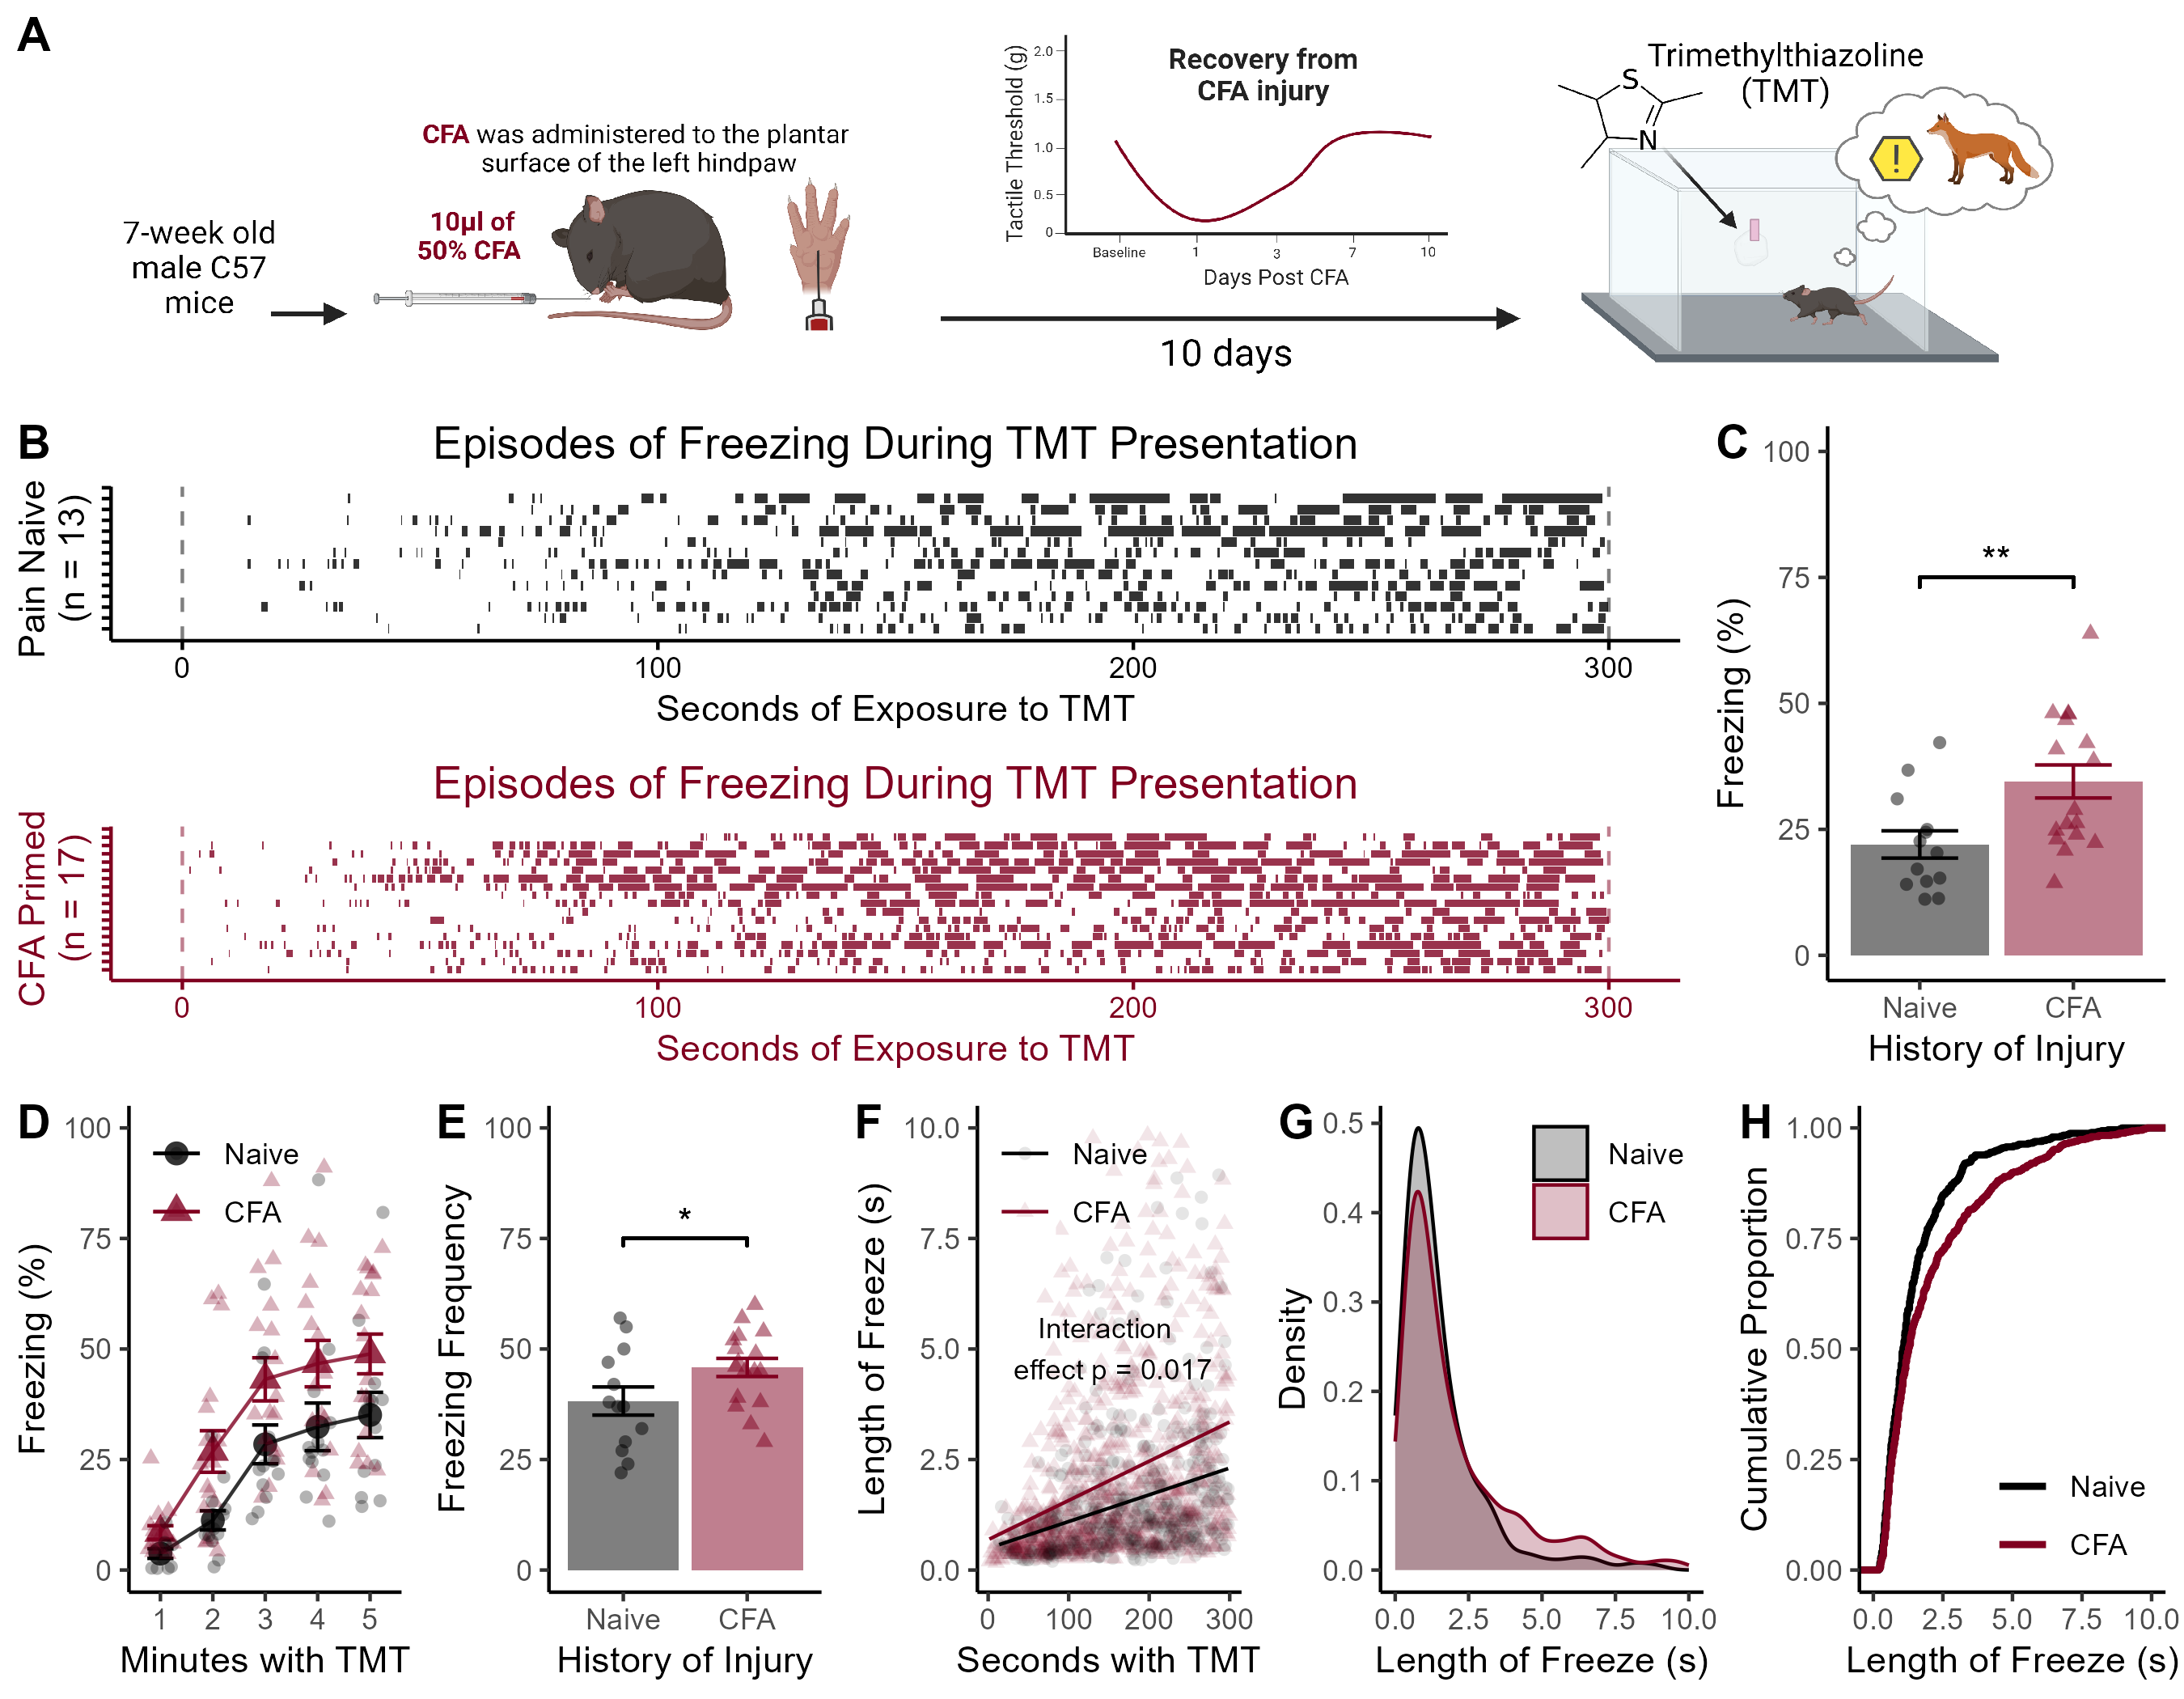
\includegraphics[width=37.5in]{Figs/1_TMT_CFA_Frz}

\textbf{Figure 1. \emph{A history of CFA injury enhances TMT-induced freezing behavior.}} (A) Timeline for behavioral testing: 10 μL of 50\% CFA injected into the footpad of the left hind paw was used as a model of injury, which produces a robust pain phenotype that reliably resolves within 7 days post-injection. Ten days after CFA, mice were tested for basal freezing levels and freezing during presentation of the single-molecule odor TMT. (B) Raster plots showing freezing behavior across the five-minute exposure to TMT. (C) CFA-primed mice spent more time freezing than pain-naive controls during TMT exposure. (D) Freezing behavior during each minute of TMT exposure. (E) Number of freezing episodes during TMT. (F) Linear relationship between time spent with TMT and length of freezing episodes. (G) Density plots showing the distribution of individual bouts of freezing compared between naive and CFA-primed mice. (H) Cumulative proportion of bouts of freezing during the TMT session. Data displayed as mean +/- SEM. ** indicates p \textless{} 0.01, *** indicates p \textless{} 0.001.

\section*{Time Spent Freezing During TMT}\label{time-spent-freezing-during-tmt}
\addcontentsline{toc}{section}{Time Spent Freezing During TMT}

\begin{Shaded}
\begin{Highlighting}[]
\NormalTok{b }\OtherTok{\textless{}{-}}\NormalTok{ Exp\_1\_CFA.N  }\SpecialCharTok{\%\textgreater{}\%}
  \FunctionTok{filter}\NormalTok{(Behavior }\SpecialCharTok{==} \StringTok{"freeze"}\NormalTok{) }\SpecialCharTok{\%\textgreater{}\%}
  \FunctionTok{group\_by}\NormalTok{(ID,CFA) }\SpecialCharTok{\%\textgreater{}\%}
  \FunctionTok{summarise}\NormalTok{(}
    \AttributeTok{sum=}\FunctionTok{sum}\NormalTok{(Duration),}
    \AttributeTok{Number=}\FunctionTok{n}\NormalTok{(),}
\NormalTok{  ) }\SpecialCharTok{\%\textgreater{}\%}
  \FunctionTok{mutate}\NormalTok{(}\AttributeTok{Perc =}\NormalTok{ (sum }\SpecialCharTok{/} \DecValTok{300}\NormalTok{)}\SpecialCharTok{*}\DecValTok{100}\NormalTok{)}
\end{Highlighting}
\end{Shaded}

\begin{verbatim}
## `summarise()` has grouped output by 'ID'. You can override using the `.groups`
## argument.
\end{verbatim}

\begin{Shaded}
\begin{Highlighting}[]
\FunctionTok{t.test}\NormalTok{(Perc}\SpecialCharTok{\textasciitilde{}}\NormalTok{CFA,}\AttributeTok{data=}\NormalTok{b,}\AttributeTok{var.equal=}\ConstantTok{TRUE}\NormalTok{)}
\end{Highlighting}
\end{Shaded}

\begin{verbatim}
## 
##  Two Sample t-test
## 
## data:  Perc by CFA
## t = -2.8169, df = 28, p-value = 0.00879
## alternative hypothesis: true difference in means between group Naive and group CFA is not equal to 0
## 95 percent confidence interval:
##  -21.59481  -3.41081
## sample estimates:
## mean in group Naive   mean in group CFA 
##            22.00138            34.50420
\end{verbatim}

Across the 5-minute exposure to TMT, mice that had previously experienced CFA spent more time freezing than did pain naive controls (\emph{t}(28) = 2.82, \emph{p} = 0.009).

\section*{Frequency of Freezing During TMT}\label{frequency-of-freezing-during-tmt}
\addcontentsline{toc}{section}{Frequency of Freezing During TMT}

\begin{Shaded}
\begin{Highlighting}[]
\FunctionTok{t.test}\NormalTok{(Number}\SpecialCharTok{\textasciitilde{}}\NormalTok{CFA,}\AttributeTok{data=}\NormalTok{b,}\AttributeTok{var.equal=}\ConstantTok{TRUE}\NormalTok{)}
\end{Highlighting}
\end{Shaded}

\begin{verbatim}
## 
##  Two Sample t-test
## 
## data:  Number by CFA
## t = -2.0875, df = 28, p-value = 0.04606
## alternative hypothesis: true difference in means between group Naive and group CFA is not equal to 0
## 95 percent confidence interval:
##  -15.0432681  -0.1422523
## sample estimates:
## mean in group Naive   mean in group CFA 
##            38.23077            45.82353
\end{verbatim}

Overall, CFA-primed mice froze more frequently than naive mice (\emph{t}(28) = 2.087, \emph{p} = 0.046).

\section*{Linear relationship between Time With TMT and Length of Freeze}\label{linear-relationship-between-time-with-tmt-and-length-of-freeze}
\addcontentsline{toc}{section}{Linear relationship between Time With TMT and Length of Freeze}

\begin{Shaded}
\begin{Highlighting}[]
\CommentTok{\# model the linear relationship between time and length of freeze}
\NormalTok{b }\OtherTok{\textless{}{-}} \FunctionTok{lm}\NormalTok{(Duration}\SpecialCharTok{\textasciitilde{}}\NormalTok{Start\_clean }\SpecialCharTok{*}\NormalTok{ CFA, }\AttributeTok{data=}\NormalTok{Exp\_1\_CFA.N)}
\FunctionTok{summary}\NormalTok{(b)}
\end{Highlighting}
\end{Shaded}

\begin{verbatim}
## 
## Call:
## lm(formula = Duration ~ Start_clean * CFA, data = Exp_1_CFA.N)
## 
## Residuals:
##     Min      1Q  Median      3Q     Max 
## -2.7754 -1.0071 -0.5278  0.1559 22.2313 
## 
## Coefficients:
##                     Estimate Std. Error t value Pr(>|t|)    
## (Intercept)         0.868308   0.158525   5.477 4.87e-08 ***
## Start_clean         0.004963   0.000912   5.442 5.92e-08 ***
## CFACFA             -0.065515   0.200135  -0.327   0.7434    
## Start_clean:CFACFA  0.002793   0.001165   2.398   0.0166 *  
## ---
## Signif. codes:  0 '***' 0.001 '**' 0.01 '*' 0.05 '.' 0.1 ' ' 1
## 
## Residual standard error: 2.068 on 1978 degrees of freedom
##   (60 observations deleted due to missingness)
## Multiple R-squared:  0.07253,    Adjusted R-squared:  0.07113 
## F-statistic: 51.56 on 3 and 1978 DF,  p-value: < 2.2e-16
\end{verbatim}

The significant interaction between time and CFA indicates that the increase in length of freezing episode across the five-minute session differs for Naive and CFA-primed mice (p = 0.01).

\begin{Shaded}
\begin{Highlighting}[]
\NormalTok{Naives }\OtherTok{\textless{}{-}}\NormalTok{ Exp\_1\_CFA.N[Exp\_1\_CFA.N}\SpecialCharTok{$}\NormalTok{CFA }\SpecialCharTok{==} \StringTok{"Naive"}\NormalTok{, ]}
\NormalTok{c }\OtherTok{\textless{}{-}} \FunctionTok{lm}\NormalTok{(Duration}\SpecialCharTok{\textasciitilde{}}\NormalTok{Start\_clean, }\AttributeTok{data =}\NormalTok{ Naives)}
\FunctionTok{summary}\NormalTok{(c)}
\end{Highlighting}
\end{Shaded}

\begin{verbatim}
## 
## Call:
## lm(formula = Duration ~ Start_clean, data = Naives)
## 
## Residuals:
##     Min      1Q  Median      3Q     Max 
## -1.8727 -0.8969 -0.4920  0.0922 22.2313 
## 
## Coefficients:
##              Estimate Std. Error t value Pr(>|t|)    
## (Intercept) 0.8683076  0.1576737   5.507 4.92e-08 ***
## Start_clean 0.0049630  0.0009071   5.471 5.97e-08 ***
## ---
## Signif. codes:  0 '***' 0.001 '**' 0.01 '*' 0.05 '.' 0.1 ' ' 1
## 
## Residual standard error: 2.057 on 803 degrees of freedom
##   (26 observations deleted due to missingness)
## Multiple R-squared:  0.03594,    Adjusted R-squared:  0.03474 
## F-statistic: 29.94 on 1 and 803 DF,  p-value: 5.967e-08
\end{verbatim}

For naive mice, a 1-second increase in time in the apparatus with TMT was associated with a 49.6 ms increase in predicted length of freeze.

\begin{Shaded}
\begin{Highlighting}[]
\NormalTok{CFAs }\OtherTok{\textless{}{-}}\NormalTok{ Exp\_1\_CFA.N[Exp\_1\_CFA.N}\SpecialCharTok{$}\NormalTok{CFA }\SpecialCharTok{==} \StringTok{"CFA"}\NormalTok{, ]}
\NormalTok{d }\OtherTok{\textless{}{-}} \FunctionTok{lm}\NormalTok{(Duration}\SpecialCharTok{\textasciitilde{}}\NormalTok{Start\_clean, }\AttributeTok{data =}\NormalTok{ CFAs)}
\FunctionTok{summary}\NormalTok{(d)}
\end{Highlighting}
\end{Shaded}

\begin{verbatim}
## 
## Call:
## lm(formula = Duration ~ Start_clean, data = CFAs)
## 
## Residuals:
##     Min      1Q  Median      3Q     Max 
## -2.7754 -1.1509 -0.5655  0.2294 15.8554 
## 
## Coefficients:
##              Estimate Std. Error t value Pr(>|t|)    
## (Intercept) 0.8027926  0.1226094   6.548 8.72e-11 ***
## Start_clean 0.0077559  0.0007271  10.667  < 2e-16 ***
## ---
## Signif. codes:  0 '***' 0.001 '**' 0.01 '*' 0.05 '.' 0.1 ' ' 1
## 
## Residual standard error: 2.076 on 1175 degrees of freedom
##   (34 observations deleted due to missingness)
## Multiple R-squared:  0.08829,    Adjusted R-squared:  0.08751 
## F-statistic: 113.8 on 1 and 1175 DF,  p-value: < 2.2e-16
\end{verbatim}

For CFA-primed mice, a 1-second increase in time spent with TMT was associated with a 77.56 ms increase in predicted length of freeze.

\begin{itemize}
\tightlist
\item
  The predicted second-by-second increase in freezing time was 56\% greater than the predicted change for naive mice.
\end{itemize}

\section*{Percent Freezing Split by Minute With TMT}\label{percent-freezing-split-by-minute-with-tmt}
\addcontentsline{toc}{section}{Percent Freezing Split by Minute With TMT}

Data binned by minute:

\begin{Shaded}
\begin{Highlighting}[]
\NormalTok{a }\OtherTok{\textless{}{-}}\NormalTok{ Exp\_1\_CFA.N }\SpecialCharTok{\%\textgreater{}\%}
  \FunctionTok{na.omit}\NormalTok{() }\SpecialCharTok{\%\textgreater{}\%}
  \FunctionTok{mutate}\NormalTok{(}\AttributeTok{Bins =} \FunctionTok{cut}\NormalTok{(}
\NormalTok{    Start\_clean,}
    \AttributeTok{breaks =} \DecValTok{5}\NormalTok{,}
    \AttributeTok{labels=}\FunctionTok{c}\NormalTok{(}\StringTok{"1"}\NormalTok{,}\StringTok{"2"}\NormalTok{,}\StringTok{"3"}\NormalTok{,}\StringTok{"4"}\NormalTok{,}\StringTok{"5"}\NormalTok{)}
\NormalTok{  )) }\SpecialCharTok{\%\textgreater{}\%}
  \FunctionTok{group\_by}\NormalTok{(ID, Behavior, CFA, PGE2, Bins) }\SpecialCharTok{\%\textgreater{}\%}
  \FunctionTok{summarise}\NormalTok{(}
    \AttributeTok{sum =} \FunctionTok{sum}\NormalTok{ (Duration)}
\NormalTok{  ) }\SpecialCharTok{\%\textgreater{}\%}
  \FunctionTok{mutate}\NormalTok{(}\AttributeTok{Perc =}\NormalTok{ (sum }\SpecialCharTok{/} \DecValTok{60}\NormalTok{)}\SpecialCharTok{*}\DecValTok{100}\NormalTok{ ) }\SpecialCharTok{\%\textgreater{}\%}
  \FunctionTok{filter}\NormalTok{(Behavior }\SpecialCharTok{==} \StringTok{"freeze"}\NormalTok{)}
\end{Highlighting}
\end{Shaded}

\begin{verbatim}
## `summarise()` has grouped output by 'ID', 'Behavior', 'CFA', 'PGE2'. You can
## override using the `.groups` argument.
\end{verbatim}

\begin{Shaded}
\begin{Highlighting}[]
\NormalTok{anova }\OtherTok{\textless{}{-}} \FunctionTok{aov}\NormalTok{(Perc}\SpecialCharTok{\textasciitilde{}}\NormalTok{Bins}\SpecialCharTok{*}\NormalTok{CFA,}\AttributeTok{data=}\NormalTok{a)}
\FunctionTok{summary}\NormalTok{(anova)}
\end{Highlighting}
\end{Shaded}

\begin{verbatim}
##              Df Sum Sq Mean Sq F value   Pr(>F)    
## Bins          4  25857    6464  22.589 2.82e-14 ***
## CFA           1   5940    5940  20.758 1.16e-05 ***
## Bins:CFA      4    483     121   0.422    0.793    
## Residuals   134  38346     286                     
## ---
## Signif. codes:  0 '***' 0.001 '**' 0.01 '*' 0.05 '.' 0.1 ' ' 1
\end{verbatim}

Freezing increased across the five minutes of exposure to TMT (F(4,134) = 22.59, p \textless{} 0.001), and CFA-primed mice froze more than naive controls (F(1,134) = 20.76, p \textless{} 0.001).

\section*{Analysis of Distribution of Length of Freezing Bouts}\label{analysis-of-distribution-of-length-of-freezing-bouts}
\addcontentsline{toc}{section}{Analysis of Distribution of Length of Freezing Bouts}

\begin{Shaded}
\begin{Highlighting}[]
\FunctionTok{library}\NormalTok{(kSamples)}

\NormalTok{a }\OtherTok{\textless{}{-}}\NormalTok{ data }\SpecialCharTok{\%\textgreater{}\%} 
  \FunctionTok{filter}\NormalTok{(CFA }\SpecialCharTok{!=} \StringTok{"CFA\_1D"}\NormalTok{) }\SpecialCharTok{\%\textgreater{}\%}
  \FunctionTok{filter}\NormalTok{(PGE2 }\SpecialCharTok{!=} \StringTok{"PGE2"}\NormalTok{) }\SpecialCharTok{\%\textgreater{}\%}
  \FunctionTok{filter}\NormalTok{(Behavior }\SpecialCharTok{==} \StringTok{"freeze"}\NormalTok{)}

\NormalTok{cfa\_durations }\OtherTok{\textless{}{-}}\NormalTok{ a}\SpecialCharTok{$}\NormalTok{Duration[a}\SpecialCharTok{$}\NormalTok{CFA }\SpecialCharTok{==} \StringTok{"CFA"}\NormalTok{]}
\NormalTok{naive\_durations }\OtherTok{\textless{}{-}}\NormalTok{ a}\SpecialCharTok{$}\NormalTok{Duration[a}\SpecialCharTok{$}\NormalTok{CFA }\SpecialCharTok{==} \StringTok{"Naive"}\NormalTok{]}

\FunctionTok{ad.test}\NormalTok{(cfa\_durations, naive\_durations)}
\end{Highlighting}
\end{Shaded}

\begin{verbatim}
## 
## 
##  Anderson-Darling k-sample test.
## 
## Number of samples:  2
## Sample sizes:  779, 497
## Number of ties: 979
## 
## Mean of  Anderson-Darling  Criterion: 1
## Standard deviation of  Anderson-Darling  Criterion: 0.76026
## 
## T.AD = ( Anderson-Darling  Criterion - mean)/sigma
## 
## Null Hypothesis: All samples come from a common population.
## 
##                AD   T.AD  asympt. P-value
## version 1: 10.595 12.621       4.7634e-06
## version 2: 10.600 12.632       4.7527e-06
\end{verbatim}

To compare the distribution of individual freezing episodes between CFA and Naive mice, an Anderson-Darling k-sample test was conducted. The test revealed a significant difference between the two distributions, (AD = 10.50, p \textless{} .001), indicating that mice with a history of CFA exhibited a shifted distribution of freezing duration compared to pain-naive mice.

\chapter*{Figure 2}\label{figure-2}
\addcontentsline{toc}{chapter}{Figure 2}

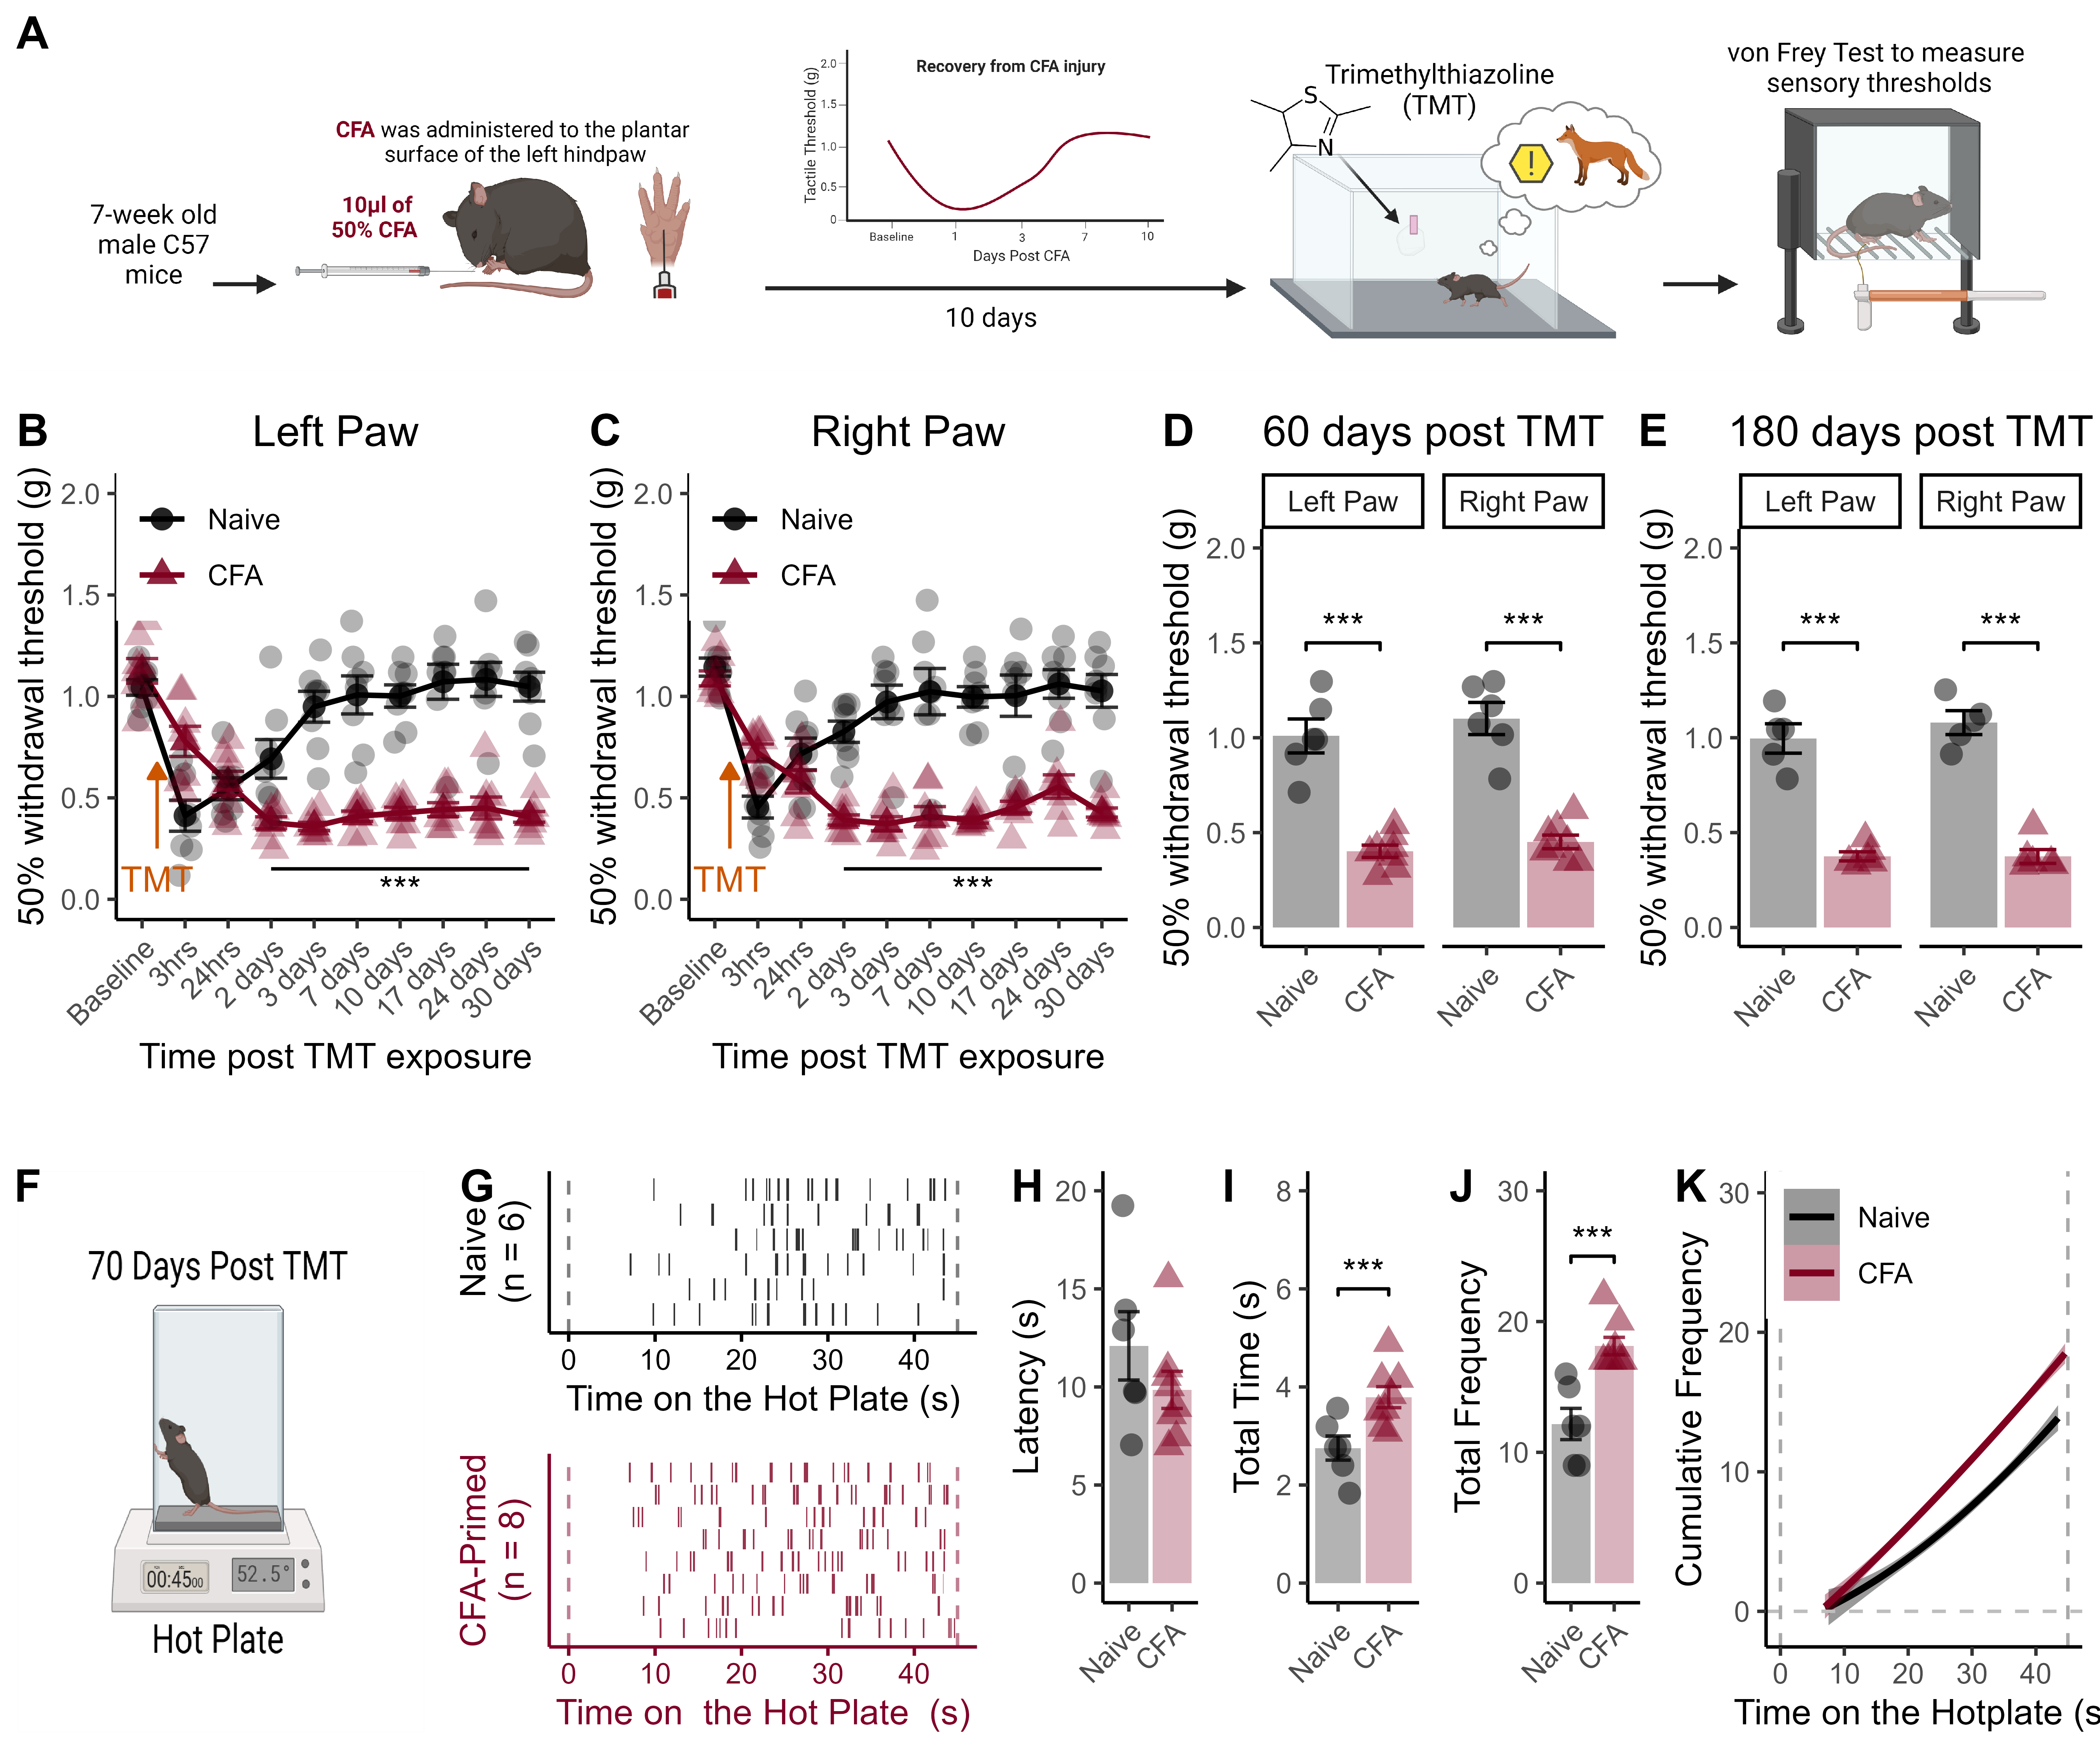
\includegraphics[width=75in]{Figs/2_TMT_VF}

\textbf{Figure 2. \emph{A history of injury facilitates chronification of TMT-induced mechanical hypersensitivity.}} (A) Timeline for behavioral testing: Naive for CFA-primed mice were exposed to TMT for five-minutes, and von Frey (VF) paw withdrawal thresholds were repeatedly measured to investigate TMT-induced alterations in sensory thresholds. (B) VF raw withdrawal thresholds after TMT in the previously injured hind paw. (C) VF paw withdrawal thresholds after TMT in the right (not injured) hindpaw. (D) VF paw withdrawal thresholds 60 days after the single exposure to TMT. (E) VF paw withdrawal thresholds 180 days after the single TMT session. (F) To further characterize the nature of the persistent hypersensitive phenotype, we used a 45 second hotplate test 70 days after the TMT exposure. (G) Raster plots showing nociceptive responses (e.g., shaking, flinching) during the hot plate test. (H) Latency to exhibit the first nociceptive response on the hot plate. (I) Mice with a history of injury spent more time exhibiting nociceptive responses. (J) The frequency of nociceptive behaviors on the hotplate was also higher for CFA-primed mice. (K) Cumulative frequency of nociceptive responses across the 45 second hot plate test. Data displayed as mean +/- SEM. *** indicates \emph{p} \textless{} 0.001.

\section*{Von Frey Paw Sensitivity After TMT}\label{von-frey-paw-sensitivity-after-tmt}
\addcontentsline{toc}{section}{Von Frey Paw Sensitivity After TMT}

\begin{Shaded}
\begin{Highlighting}[]
\CommentTok{\# Left}
\NormalTok{a }\OtherTok{\textless{}{-}}\NormalTok{ Left\_Data }\SpecialCharTok{\%\textgreater{}\%}
  \FunctionTok{melt}\NormalTok{(}\AttributeTok{id.vars =} \FunctionTok{c}\NormalTok{(}\StringTok{"ID"}\NormalTok{, }\StringTok{"Condition"}\NormalTok{)) }\SpecialCharTok{\%\textgreater{}\%}
  \FunctionTok{na.omit}\NormalTok{()}

\FunctionTok{anova\_test}\NormalTok{(}\AttributeTok{data =}\NormalTok{ a, }\AttributeTok{within =}\NormalTok{ variable, }\AttributeTok{dv =}\NormalTok{ value, }\AttributeTok{between =}\NormalTok{ Condition, }\AttributeTok{wid =}\NormalTok{ ID)}
\end{Highlighting}
\end{Shaded}

\begin{verbatim}
## ANOVA Table (type II tests)
## 
## $ANOVA
##               Effect DFn DFd      F        p p<.05   ges
## 1          Condition   1  14 46.740 8.10e-06     * 0.567
## 2           variable   9 126 21.226 1.93e-21     * 0.479
## 3 Condition:variable   9 126 30.857 7.38e-28     * 0.572
## 
## $`Mauchly's Test for Sphericity`
##               Effect     W     p p<.05
## 1           variable 0.017 0.548      
## 2 Condition:variable 0.017 0.548      
## 
## $`Sphericity Corrections`
##               Effect   GGe      DF[GG]    p[GG] p[GG]<.05   HFe       DF[HF]
## 1           variable 0.579 5.22, 73.01 2.56e-13         * 0.964 8.68, 121.48
## 2 Condition:variable 0.579 5.22, 73.01 4.62e-17         * 0.964 8.68, 121.48
##      p[HF] p[HF]<.05
## 1 9.48e-21         *
## 2 6.13e-27         *
\end{verbatim}

\begin{Shaded}
\begin{Highlighting}[]
\CommentTok{\# Right}
\NormalTok{a }\OtherTok{\textless{}{-}}\NormalTok{ Right\_Data }\SpecialCharTok{\%\textgreater{}\%}
  \FunctionTok{melt}\NormalTok{(}\AttributeTok{id.vars =} \FunctionTok{c}\NormalTok{(}\StringTok{"ID"}\NormalTok{, }\StringTok{"Condition"}\NormalTok{)) }\SpecialCharTok{\%\textgreater{}\%}
  \FunctionTok{na.omit}\NormalTok{()}

\FunctionTok{anova\_test}\NormalTok{(}\AttributeTok{data =}\NormalTok{ a, }\AttributeTok{within =}\NormalTok{ variable, }\AttributeTok{dv =}\NormalTok{ value, }\AttributeTok{between =}\NormalTok{ Condition, }\AttributeTok{wid =}\NormalTok{ ID)}
\end{Highlighting}
\end{Shaded}

\begin{verbatim}
## ANOVA Table (type II tests)
## 
## $ANOVA
##               Effect DFn DFd      F        p p<.05   ges
## 1          Condition   1  14 80.560 3.50e-07     * 0.621
## 2           variable   9 126 17.556 1.50e-18     * 0.473
## 3 Condition:variable   9 126 18.129 5.08e-19     * 0.481
## 
## $`Mauchly's Test for Sphericity`
##               Effect     W     p p<.05
## 1           variable 0.004 0.104      
## 2 Condition:variable 0.004 0.104      
## 
## $`Sphericity Corrections`
##               Effect   GGe      DF[GG]    p[GG] p[GG]<.05   HFe    DF[HF]
## 1           variable 0.486 4.37, 61.19 4.50e-10         * 0.733 6.6, 92.4
## 2 Condition:variable 0.486 4.37, 61.19 2.64e-10         * 0.733 6.6, 92.4
##      p[HF] p[HF]<.05
## 1 3.62e-14         *
## 2 1.63e-14         *
\end{verbatim}

We measured von Frey (VF) paw withdrawal thresholds after TMT exposure to assess whether synthetic predator threat alters peripheral mechanical sensitivity (Figure 2A). A single five-minute exposure to TMT induced changes in paw withdrawal thresholds in the left (F9,126 = 21.23, p \textless{} 0.001, Figure 2B) and right (F9,126 = 17.56, p \textless{} 0.001, Figure 2C) hind paws that differed for pain-naive and CFA primed mice (Left hind paws: F9,126 = 30.86 p \textless{} 0.001; Right hind paws: F9,126 = 18.13, p \textless{} 0.001).

\begin{Shaded}
\begin{Highlighting}[]
\DocumentationTok{\#\# Left Paws}
\NormalTok{a }\OtherTok{\textless{}{-}}\NormalTok{ Left\_Data }\SpecialCharTok{\%\textgreater{}\%}
  \FunctionTok{melt}\NormalTok{(}\AttributeTok{id.vars =} \FunctionTok{c}\NormalTok{(}\StringTok{"ID"}\NormalTok{,}\StringTok{"Condition"}\NormalTok{,}\StringTok{"Baseline"}\NormalTok{)) }\SpecialCharTok{\%\textgreater{}\%}
  \FunctionTok{mutate}\NormalTok{(}\AttributeTok{Perc\_BL =}\NormalTok{ value }\SpecialCharTok{/}\NormalTok{ Baseline }\SpecialCharTok{*} \DecValTok{100}\NormalTok{) }
  
\FunctionTok{anova\_test}\NormalTok{(}\AttributeTok{data =}\NormalTok{ a, }\AttributeTok{dv =}\NormalTok{ Perc\_BL, }\AttributeTok{between =}\NormalTok{ Condition, }\AttributeTok{within =}\NormalTok{ variable, }\AttributeTok{wid =}\NormalTok{ ID)}
\end{Highlighting}
\end{Shaded}

\begin{verbatim}
## ANOVA Table (type II tests)
## 
## $ANOVA
##               Effect DFn DFd      F        p p<.05   ges
## 1          Condition   1  14 87.365 2.14e-07     * 0.670
## 2           variable   8 112  6.793 3.03e-07     * 0.247
## 3 Condition:variable   8 112 26.260 1.90e-22     * 0.559
## 
## $`Mauchly's Test for Sphericity`
##               Effect     W     p p<.05
## 1           variable 0.015 0.114      
## 2 Condition:variable 0.015 0.114      
## 
## $`Sphericity Corrections`
##               Effect   GGe      DF[GG]    p[GG] p[GG]<.05   HFe      DF[HF]
## 1           variable 0.499 3.99, 55.91 1.59e-04         * 0.723 5.79, 81.02
## 2 Condition:variable 0.499 3.99, 55.91 2.86e-12         * 0.723 5.79, 81.02
##      p[HF] p[HF]<.05
## 1 9.44e-06         *
## 2 7.74e-17         *
\end{verbatim}

\begin{Shaded}
\begin{Highlighting}[]
\NormalTok{a }\SpecialCharTok{\%\textgreater{}\%}
\NormalTok{  dplyr}\SpecialCharTok{::}\FunctionTok{group\_by}\NormalTok{(Condition) }\SpecialCharTok{\%\textgreater{}\%}
  \FunctionTok{pairwise\_t\_test}\NormalTok{(value }\SpecialCharTok{\textasciitilde{}}\NormalTok{ variable) }\SpecialCharTok{\%\textgreater{}\%}
  \FunctionTok{filter}\NormalTok{(group1 }\SpecialCharTok{==} \StringTok{"Baseline"}\NormalTok{)}
\end{Highlighting}
\end{Shaded}

\begin{verbatim}
## # A tibble: 0 x 10
## # i 10 variables: Condition <fct>, .y. <chr>, group1 <chr>, group2 <chr>,
## #   n1 <int>, n2 <int>, p <dbl>, p.signif <chr>, p.adj <dbl>,
## #   p.adj.signif <chr>
\end{verbatim}

\begin{Shaded}
\begin{Highlighting}[]
\DocumentationTok{\#\# Right Paws}
\NormalTok{a }\OtherTok{\textless{}{-}}\NormalTok{ Right\_Data }\SpecialCharTok{\%\textgreater{}\%}
  \FunctionTok{melt}\NormalTok{(}\AttributeTok{id.vars =} \FunctionTok{c}\NormalTok{(}\StringTok{"ID"}\NormalTok{,}\StringTok{"Condition"}\NormalTok{,}\StringTok{"Baseline"}\NormalTok{)) }\SpecialCharTok{\%\textgreater{}\%}
  \FunctionTok{mutate}\NormalTok{(}\AttributeTok{Perc\_BL =}\NormalTok{ value }\SpecialCharTok{/}\NormalTok{ Baseline }\SpecialCharTok{*} \DecValTok{100}\NormalTok{) }
  
\FunctionTok{anova\_test}\NormalTok{(}\AttributeTok{data =}\NormalTok{ a, }\AttributeTok{dv =}\NormalTok{ Perc\_BL, }\AttributeTok{between =}\NormalTok{ Condition, }\AttributeTok{within =}\NormalTok{ variable, }\AttributeTok{wid =}\NormalTok{ ID)}
\end{Highlighting}
\end{Shaded}

\begin{verbatim}
## ANOVA Table (type II tests)
## 
## $ANOVA
##               Effect DFn DFd      F        p p<.05   ges
## 1          Condition   1  14 32.047 5.88e-05     * 0.553
## 2           variable   8 112  4.034 3.05e-04     * 0.117
## 3 Condition:variable   8 112 19.234 6.18e-18     * 0.388
## 
## $`Mauchly's Test for Sphericity`
##               Effect     W     p p<.05
## 1           variable 0.026 0.286      
## 2 Condition:variable 0.026 0.286      
## 
## $`Sphericity Corrections`
##               Effect   GGe     DF[GG]    p[GG] p[GG]<.05  HFe       DF[HF]
## 1           variable 0.596 4.76, 66.7 3.00e-03         * 0.94 7.52, 105.29
## 2 Condition:variable 0.596 4.76, 66.7 1.59e-11         * 0.94 7.52, 105.29
##      p[HF] p[HF]<.05
## 1 4.34e-04         *
## 2 5.46e-17         *
\end{verbatim}

\begin{Shaded}
\begin{Highlighting}[]
\NormalTok{a }\SpecialCharTok{\%\textgreater{}\%}
\NormalTok{  dplyr}\SpecialCharTok{::}\FunctionTok{group\_by}\NormalTok{(Condition) }\SpecialCharTok{\%\textgreater{}\%}
  \FunctionTok{pairwise\_t\_test}\NormalTok{(value }\SpecialCharTok{\textasciitilde{}}\NormalTok{ variable) }\SpecialCharTok{\%\textgreater{}\%}
  \FunctionTok{filter}\NormalTok{(group1 }\SpecialCharTok{==} \StringTok{"Baseline"}\NormalTok{)}
\end{Highlighting}
\end{Shaded}

\begin{verbatim}
## # A tibble: 0 x 10
## # i 10 variables: Condition <fct>, .y. <chr>, group1 <chr>, group2 <chr>,
## #   n1 <int>, n2 <int>, p <dbl>, p.signif <chr>, p.adj <dbl>,
## #   p.adj.signif <chr>
\end{verbatim}

For pain-naive mice, TMT-induced mechanical hypersensitivity resolved three days after exposure (left hind paws: all p \textgreater{} 0.32; right hind paws: all p \textgreater{} 0.15, relative to baseline measurements). In contrast, CFA-primed mice exhibited a persistent state of mechanical hypersensitivity after TMT exposure that did not resolve. The ongoing mechanical hypersensitivity expressed by CFA-primed mice was present both in the previously injured (left) hind paw (all p \textless{} 0.012 relative to baseline measurements) and in the not-previously-injured right hind paw (all p \textless{} 0.001 relative to baseline measurements).

\begin{Shaded}
\begin{Highlighting}[]
\CommentTok{\# 60 Days}
\FunctionTok{t.test}\NormalTok{(}\AttributeTok{data =}\NormalTok{ no\_1D,  L\_60D }\SpecialCharTok{\textasciitilde{}}\NormalTok{ Condition, }\AttributeTok{var.equal =}\NormalTok{ T)}
\end{Highlighting}
\end{Shaded}

\begin{verbatim}
## 
##  Two Sample t-test
## 
## data:  L_60D by Condition
## t = 7.761, df = 12, p-value = 5.122e-06
## alternative hypothesis: true difference in means between group Naive and group CFA is not equal to 0
## 95 percent confidence interval:
##  0.4373241 0.7787102
## sample estimates:
## mean in group Naive   mean in group CFA 
##           1.0093144           0.4012973
\end{verbatim}

\begin{Shaded}
\begin{Highlighting}[]
\FunctionTok{t.test}\NormalTok{(}\AttributeTok{data =}\NormalTok{ no\_1D, R\_60D }\SpecialCharTok{\textasciitilde{}}\NormalTok{ Condition, }\AttributeTok{var.equal =}\NormalTok{ T)}
\end{Highlighting}
\end{Shaded}

\begin{verbatim}
## 
##  Two Sample t-test
## 
## data:  R_60D by Condition
## t = 8.4717, df = 12, p-value = 2.082e-06
## alternative hypothesis: true difference in means between group Naive and group CFA is not equal to 0
## 95 percent confidence interval:
##  0.4831440 0.8177076
## sample estimates:
## mean in group Naive   mean in group CFA 
##           1.1013267           0.4509009
\end{verbatim}

Sixty days after the single TMT exposure, CFA-primed mice continued to exhibit lower paw withdrawal thresholds than pain-naive controls (F1,12 = 112.02, p \textless{} 0.001, Figure 2D), and the hypersensitivity did not differ between the right and left hind paws (p = 0.68).

\begin{Shaded}
\begin{Highlighting}[]
\CommentTok{\# 180 Days}
\FunctionTok{t.test}\NormalTok{(}\AttributeTok{data =}\NormalTok{ no\_1D, L\_180D }\SpecialCharTok{\textasciitilde{}}\NormalTok{ Condition, }\AttributeTok{var.equal =}\NormalTok{ T)}
\end{Highlighting}
\end{Shaded}

\begin{verbatim}
## 
##  Two Sample t-test
## 
## data:  L_180D by Condition
## t = 9.2569, df = 9, p-value = 6.778e-06
## alternative hypothesis: true difference in means between group Naive and group CFA is not equal to 0
## 95 percent confidence interval:
##  0.4694201 0.7730487
## sample estimates:
## mean in group Naive   mean in group CFA 
##           0.9960839           0.3748495
\end{verbatim}

\begin{Shaded}
\begin{Highlighting}[]
\FunctionTok{t.test}\NormalTok{(}\AttributeTok{data =}\NormalTok{ no\_1D, R\_180D }\SpecialCharTok{\textasciitilde{}}\NormalTok{ Condition, }\AttributeTok{var.equal =}\NormalTok{ T)}
\end{Highlighting}
\end{Shaded}

\begin{verbatim}
## 
##  Two Sample t-test
## 
## data:  R_180D by Condition
## t = 11.236, df = 9, p-value = 1.346e-06
## alternative hypothesis: true difference in means between group Naive and group CFA is not equal to 0
## 95 percent confidence interval:
##  0.5633834 0.8474259
## sample estimates:
## mean in group Naive   mean in group CFA 
##           1.0796716           0.3742669
\end{verbatim}

The hypersensitivity remained detectable among CFA-primed mice 180 days after the single exposure (F1,9 = 165.45, p \textless{} 0.001, Figure 2E) for both hind paws.

\section*{Hot Plate Test}\label{hot-plate-test}
\addcontentsline{toc}{section}{Hot Plate Test}

\begin{Shaded}
\begin{Highlighting}[]
\CommentTok{\# Latency to shake / flick}
\NormalTok{a }\OtherTok{\textless{}{-}}\NormalTok{ data }\SpecialCharTok{\%\textgreater{}\%}
  \FunctionTok{group\_by}\NormalTok{(ID,CFA) }\SpecialCharTok{\%\textgreater{}\%}
  \FunctionTok{filter}\NormalTok{(Behavior }\SpecialCharTok{==} \StringTok{"shake"}\NormalTok{) }\SpecialCharTok{\%\textgreater{}\%}
  \FunctionTok{filter}\NormalTok{(CFA }\SpecialCharTok{!=} \StringTok{"CFA\_1\_day"}\NormalTok{) }\SpecialCharTok{\%\textgreater{}\%}
  \FunctionTok{summarise}\NormalTok{(}
    \AttributeTok{min=}\FunctionTok{min}\NormalTok{(Start\_clean)}
\NormalTok{  )}
\end{Highlighting}
\end{Shaded}

\begin{verbatim}
## `summarise()` has grouped output by 'ID'. You can override using the `.groups`
## argument.
\end{verbatim}

\begin{Shaded}
\begin{Highlighting}[]
\FunctionTok{t.test}\NormalTok{(}\AttributeTok{data =}\NormalTok{ a, min }\SpecialCharTok{\textasciitilde{}}\NormalTok{ CFA,}\AttributeTok{var.equal =} \ConstantTok{TRUE}\NormalTok{)}
\end{Highlighting}
\end{Shaded}

\begin{verbatim}
## 
##  Two Sample t-test
## 
## data:  min by CFA
## t = 1.2107, df = 12, p-value = 0.2493
## alternative hypothesis: true difference in means between group TMT_Only and group CFA_10_days is not equal to 0
## 95 percent confidence interval:
##  -1.794543  6.282959
## sample estimates:
##    mean in group TMT_Only mean in group CFA_10_days 
##                 12.094333                  9.850125
\end{verbatim}

There was no group difference in the latency to first nociceptive response (p = 0.25 Figure 2G,H).

\begin{Shaded}
\begin{Highlighting}[]
\CommentTok{\# Total time spent exhibiting nociceptive responses}
\NormalTok{a }\OtherTok{\textless{}{-}}\NormalTok{ data }\SpecialCharTok{\%\textgreater{}\%}
  \FunctionTok{group\_by}\NormalTok{(ID,CFA) }\SpecialCharTok{\%\textgreater{}\%}
  \FunctionTok{filter}\NormalTok{(Behavior }\SpecialCharTok{==} \StringTok{"shake"}\NormalTok{) }\SpecialCharTok{\%\textgreater{}\%}
  \FunctionTok{filter}\NormalTok{(CFA }\SpecialCharTok{!=} \StringTok{"CFA\_1\_day"}\NormalTok{) }\SpecialCharTok{\%\textgreater{}\%}
  \FunctionTok{summarise}\NormalTok{(}
    \AttributeTok{sum=}\FunctionTok{sum}\NormalTok{(Duration)}
\NormalTok{  )}
\end{Highlighting}
\end{Shaded}

\begin{verbatim}
## `summarise()` has grouped output by 'ID'. You can override using the `.groups`
## argument.
\end{verbatim}

\begin{Shaded}
\begin{Highlighting}[]
\FunctionTok{t.test}\NormalTok{(}\AttributeTok{data =}\NormalTok{ a, sum }\SpecialCharTok{\textasciitilde{}}\NormalTok{ CFA,}\AttributeTok{var.equal =} \ConstantTok{TRUE}\NormalTok{)}
\end{Highlighting}
\end{Shaded}

\begin{verbatim}
## 
##  Two Sample t-test
## 
## data:  sum by CFA
## t = -3.1747, df = 12, p-value = 0.008
## alternative hypothesis: true difference in means between group TMT_Only and group CFA_10_days is not equal to 0
## 95 percent confidence interval:
##  -1.7494097 -0.3254236
## sample estimates:
##    mean in group TMT_Only mean in group CFA_10_days 
##                  2.753833                  3.791250
\end{verbatim}

CFA-primed mice spent significantly more time displaying pain-related behaviors (t12 = 3.17, p = 0.008, Figure 2I)

\begin{Shaded}
\begin{Highlighting}[]
\CommentTok{\# Frequency of nociceptive responses}
\NormalTok{a }\OtherTok{\textless{}{-}}\NormalTok{ data }\SpecialCharTok{\%\textgreater{}\%}
  \FunctionTok{group\_by}\NormalTok{(ID,CFA) }\SpecialCharTok{\%\textgreater{}\%}
  \FunctionTok{filter}\NormalTok{(Behavior }\SpecialCharTok{==} \StringTok{"shake"}\NormalTok{) }\SpecialCharTok{\%\textgreater{}\%}
  \FunctionTok{filter}\NormalTok{(CFA }\SpecialCharTok{!=} \StringTok{"CFA\_1\_day"}\NormalTok{) }\SpecialCharTok{\%\textgreater{}\%}
  \FunctionTok{summarise}\NormalTok{(}
    \AttributeTok{n=}\FunctionTok{n}\NormalTok{()}
\NormalTok{  )}
\end{Highlighting}
\end{Shaded}

\begin{verbatim}
## `summarise()` has grouped output by 'ID'. You can override using the `.groups`
## argument.
\end{verbatim}

\begin{Shaded}
\begin{Highlighting}[]
\FunctionTok{t.test}\NormalTok{(}\AttributeTok{data =}\NormalTok{ a, n }\SpecialCharTok{\textasciitilde{}}\NormalTok{ CFA,}\AttributeTok{var.equal =} \ConstantTok{TRUE}\NormalTok{)}
\end{Highlighting}
\end{Shaded}

\begin{verbatim}
## 
##  Two Sample t-test
## 
## data:  n by CFA
## t = -4.6446, df = 12, p-value = 0.0005657
## alternative hypothesis: true difference in means between group TMT_Only and group CFA_10_days is not equal to 0
## 95 percent confidence interval:
##  -8.753410 -3.163256
## sample estimates:
##    mean in group TMT_Only mean in group CFA_10_days 
##                  12.16667                  18.12500
\end{verbatim}

and exhibited a higher frequency of pain responses (t12 = 4.64, p \textless{} 0.0001, Figure 2J,K) during the 45-second task.

In separate experiments, we replicated the same experimental setup, but exposed mice to the odor butyric acid (an odor that is repugnant but not fear-inducing) instead of TMT. We found that mice did not exhibit freezing behavior or mechanical hypersensitivity after butyric acid exposure (Figure S3), highlighting that the behavioral responses to TMT represent a specific fear response, and are not related to the other elements of the testing procedures.

\chapter*{Figure 3}\label{figure-3}
\addcontentsline{toc}{chapter}{Figure 3}

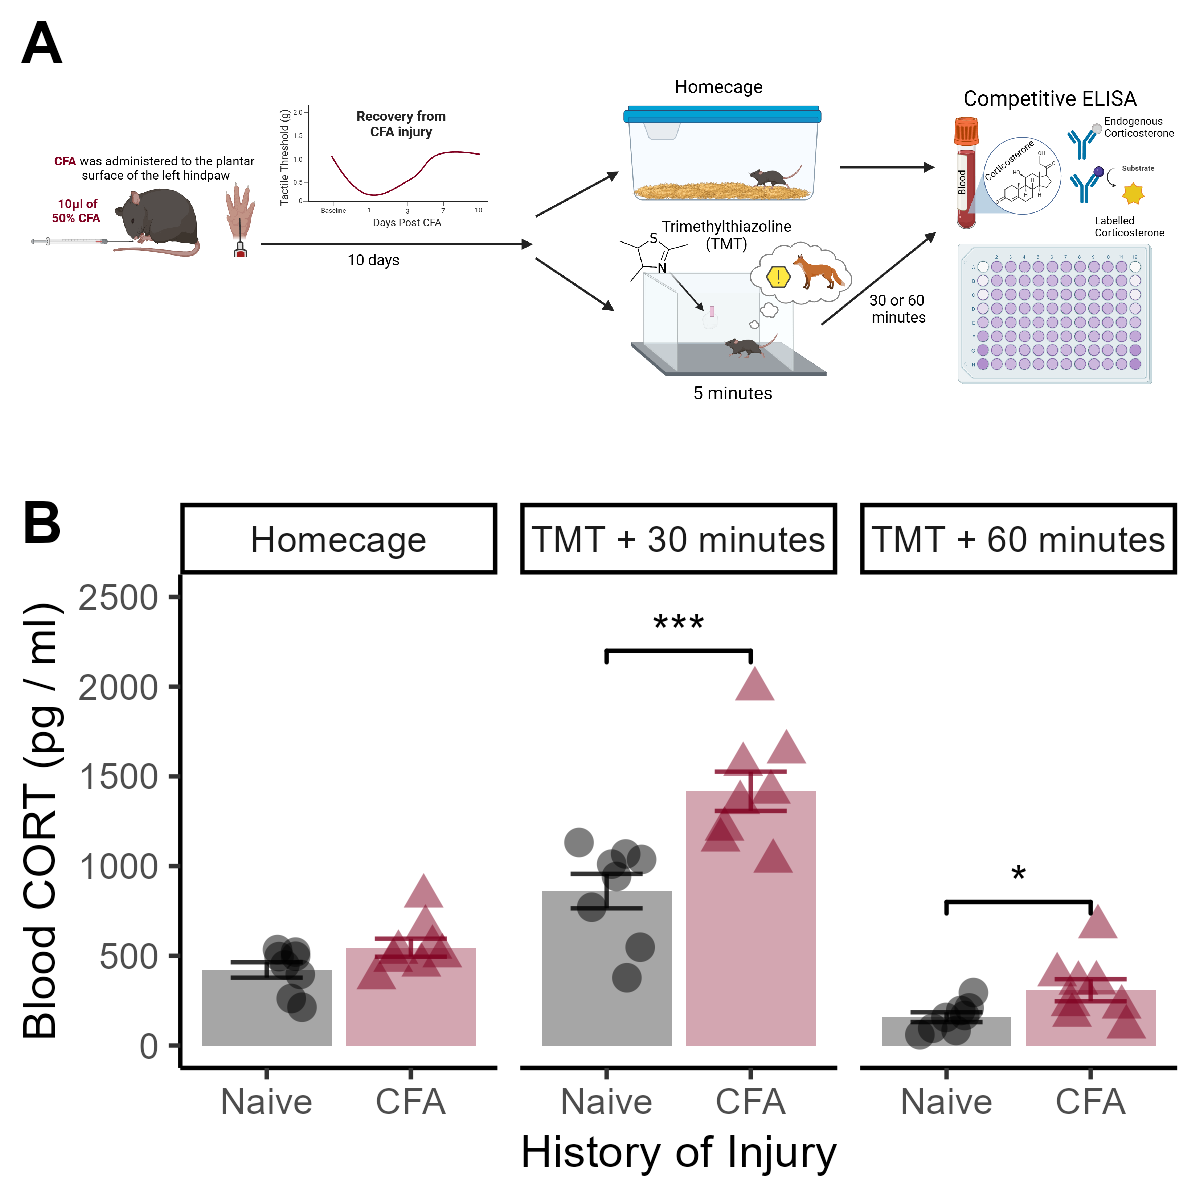
\includegraphics[width=16.67in]{Figs/3_CORT}

\textbf{Figure 3. \emph{Mice with a history of injury have higher levels of blood corticosterone after TMT exposure.}} (A) Timeline of experimental procedures. Mice were injected with CFA, allowed 10 days for their injury to recover, and were then exposed to TMT for 5 minutes. Either 30 or 60 minutes after TMT, trunk blood was collected. (B) Although there is no difference in basal levels of blood corticosterone, CFA-primed mice exhibited higher levels of circulating corticosterone at both 30 and 60 minutes after TMT. Data presented as mean +/- SEM. * indicates \emph{p} \textless{} 0.05, *** indicates \emph{p} \textless{} 0.001.

\section*{Overall Effects of Stress and Timepoint}\label{overall-effects-of-stress-and-timepoint}
\addcontentsline{toc}{section}{Overall Effects of Stress and Timepoint}

\begin{Shaded}
\begin{Highlighting}[]
\NormalTok{res }\OtherTok{\textless{}{-}} \FunctionTok{aov}\NormalTok{(CORT }\SpecialCharTok{\textasciitilde{}}\NormalTok{ Stress }\SpecialCharTok{*}\NormalTok{ Pain, }\AttributeTok{data =}\NormalTok{ data)}
\FunctionTok{summary}\NormalTok{(res)}
\end{Highlighting}
\end{Shaded}

\begin{verbatim}
##             Df  Sum Sq Mean Sq F value   Pr(>F)    
## Stress       2 7000783 3500391  87.218 1.11e-15 ***
## Pain         1  919426  919426  22.909 2.12e-05 ***
## Stress:Pain  2  469721  234860   5.852  0.00573 ** 
## Residuals   42 1685623   40134                     
## ---
## Signif. codes:  0 '***' 0.001 '**' 0.01 '*' 0.05 '.' 0.1 ' ' 1
\end{verbatim}

\section*{Follow Ups: Effect of CFA at Each Timepoint}\label{follow-ups-effect-of-cfa-at-each-timepoint}
\addcontentsline{toc}{section}{Follow Ups: Effect of CFA at Each Timepoint}

\begin{Shaded}
\begin{Highlighting}[]
\CommentTok{\# Basal}
\NormalTok{a }\OtherTok{\textless{}{-}}\NormalTok{ data }\SpecialCharTok{\%\textgreater{}\%}
  \FunctionTok{select}\NormalTok{(}\FunctionTok{c}\NormalTok{(}\StringTok{"ID"}\NormalTok{,}\StringTok{"Pain"}\NormalTok{,}\StringTok{"Stress"}\NormalTok{,}\StringTok{"CORT"}\NormalTok{)) }\SpecialCharTok{\%\textgreater{}\%}
  \FunctionTok{filter}\NormalTok{(Stress }\SpecialCharTok{==} \StringTok{"Homecage"}\NormalTok{)}
  
\FunctionTok{t.test}\NormalTok{(CORT }\SpecialCharTok{\textasciitilde{}}\NormalTok{ Pain, }\AttributeTok{data =}\NormalTok{ a, }\AttributeTok{var.equal =}\NormalTok{ T)}
\end{Highlighting}
\end{Shaded}

\begin{verbatim}
## 
##  Two Sample t-test
## 
## data:  CORT by Pain
## t = -1.8737, df = 14, p-value = 0.082
## alternative hypothesis: true difference in means between group Naive and group CFA is not equal to 0
## 95 percent confidence interval:
##  -265.92402   17.94027
## sample estimates:
## mean in group Naive   mean in group CFA 
##            421.1277            545.1196
\end{verbatim}

Competitive ELISA results showed no significant difference in basal corticosterone levels between groups (p = 0.08).

\begin{Shaded}
\begin{Highlighting}[]
\CommentTok{\# 30 minutes after TMT}
\NormalTok{a }\OtherTok{\textless{}{-}}\NormalTok{ data }\SpecialCharTok{\%\textgreater{}\%}
  \FunctionTok{select}\NormalTok{(}\FunctionTok{c}\NormalTok{(}\StringTok{"ID"}\NormalTok{,}\StringTok{"Pain"}\NormalTok{,}\StringTok{"Stress"}\NormalTok{,}\StringTok{"CORT"}\NormalTok{)) }\SpecialCharTok{\%\textgreater{}\%}
  \FunctionTok{filter}\NormalTok{(Stress }\SpecialCharTok{==} \StringTok{"TMT\_30"}\NormalTok{)}
  
\FunctionTok{t.test}\NormalTok{(CORT }\SpecialCharTok{\textasciitilde{}}\NormalTok{ Pain, }\AttributeTok{data =}\NormalTok{ a, }\AttributeTok{var.equal =}\NormalTok{ T)}
\end{Highlighting}
\end{Shaded}

\begin{verbatim}
## 
##  Two Sample t-test
## 
## data:  CORT by Pain
## t = -3.8218, df = 14, p-value = 0.001869
## alternative hypothesis: true difference in means between group Naive and group CFA is not equal to 0
## 95 percent confidence interval:
##  -868.3244 -244.0529
## sample estimates:
## mean in group Naive   mean in group CFA 
##            860.6665           1416.8552
\end{verbatim}

\begin{Shaded}
\begin{Highlighting}[]
\CommentTok{\# 60 minutes after TMT}
\NormalTok{a }\OtherTok{\textless{}{-}}\NormalTok{ data }\SpecialCharTok{\%\textgreater{}\%}
  \FunctionTok{select}\NormalTok{(}\FunctionTok{c}\NormalTok{(}\StringTok{"ID"}\NormalTok{,}\StringTok{"Pain"}\NormalTok{,}\StringTok{"Stress"}\NormalTok{,}\StringTok{"CORT"}\NormalTok{)) }\SpecialCharTok{\%\textgreater{}\%}
  \FunctionTok{filter}\NormalTok{(Stress }\SpecialCharTok{==} \StringTok{"TMT\_60"}\NormalTok{)}
  
\FunctionTok{t.test}\NormalTok{(CORT }\SpecialCharTok{\textasciitilde{}}\NormalTok{ Pain, }\AttributeTok{data =}\NormalTok{ a, }\AttributeTok{var.equal =}\NormalTok{ T)}
\end{Highlighting}
\end{Shaded}

\begin{verbatim}
## 
##  Two Sample t-test
## 
## data:  CORT by Pain
## t = -2.2291, df = 14, p-value = 0.0427
## alternative hypothesis: true difference in means between group Naive and group CFA is not equal to 0
## 95 percent confidence interval:
##  -294.762456   -5.683044
## sample estimates:
## mean in group Naive   mean in group CFA 
##            157.9656            308.1883
\end{verbatim}

However, both 30 and 60 minutes post-TMT, CFA-primed mice exhibited significantly higher circulating corticosterone levels compared to pain-naive controls (t14 = 3.82, p = 0.0018, t14 = 2.22, p = 0.043, respectively, Figure 3B).

\chapter*{Figure 4}\label{figure-4}
\addcontentsline{toc}{chapter}{Figure 4}

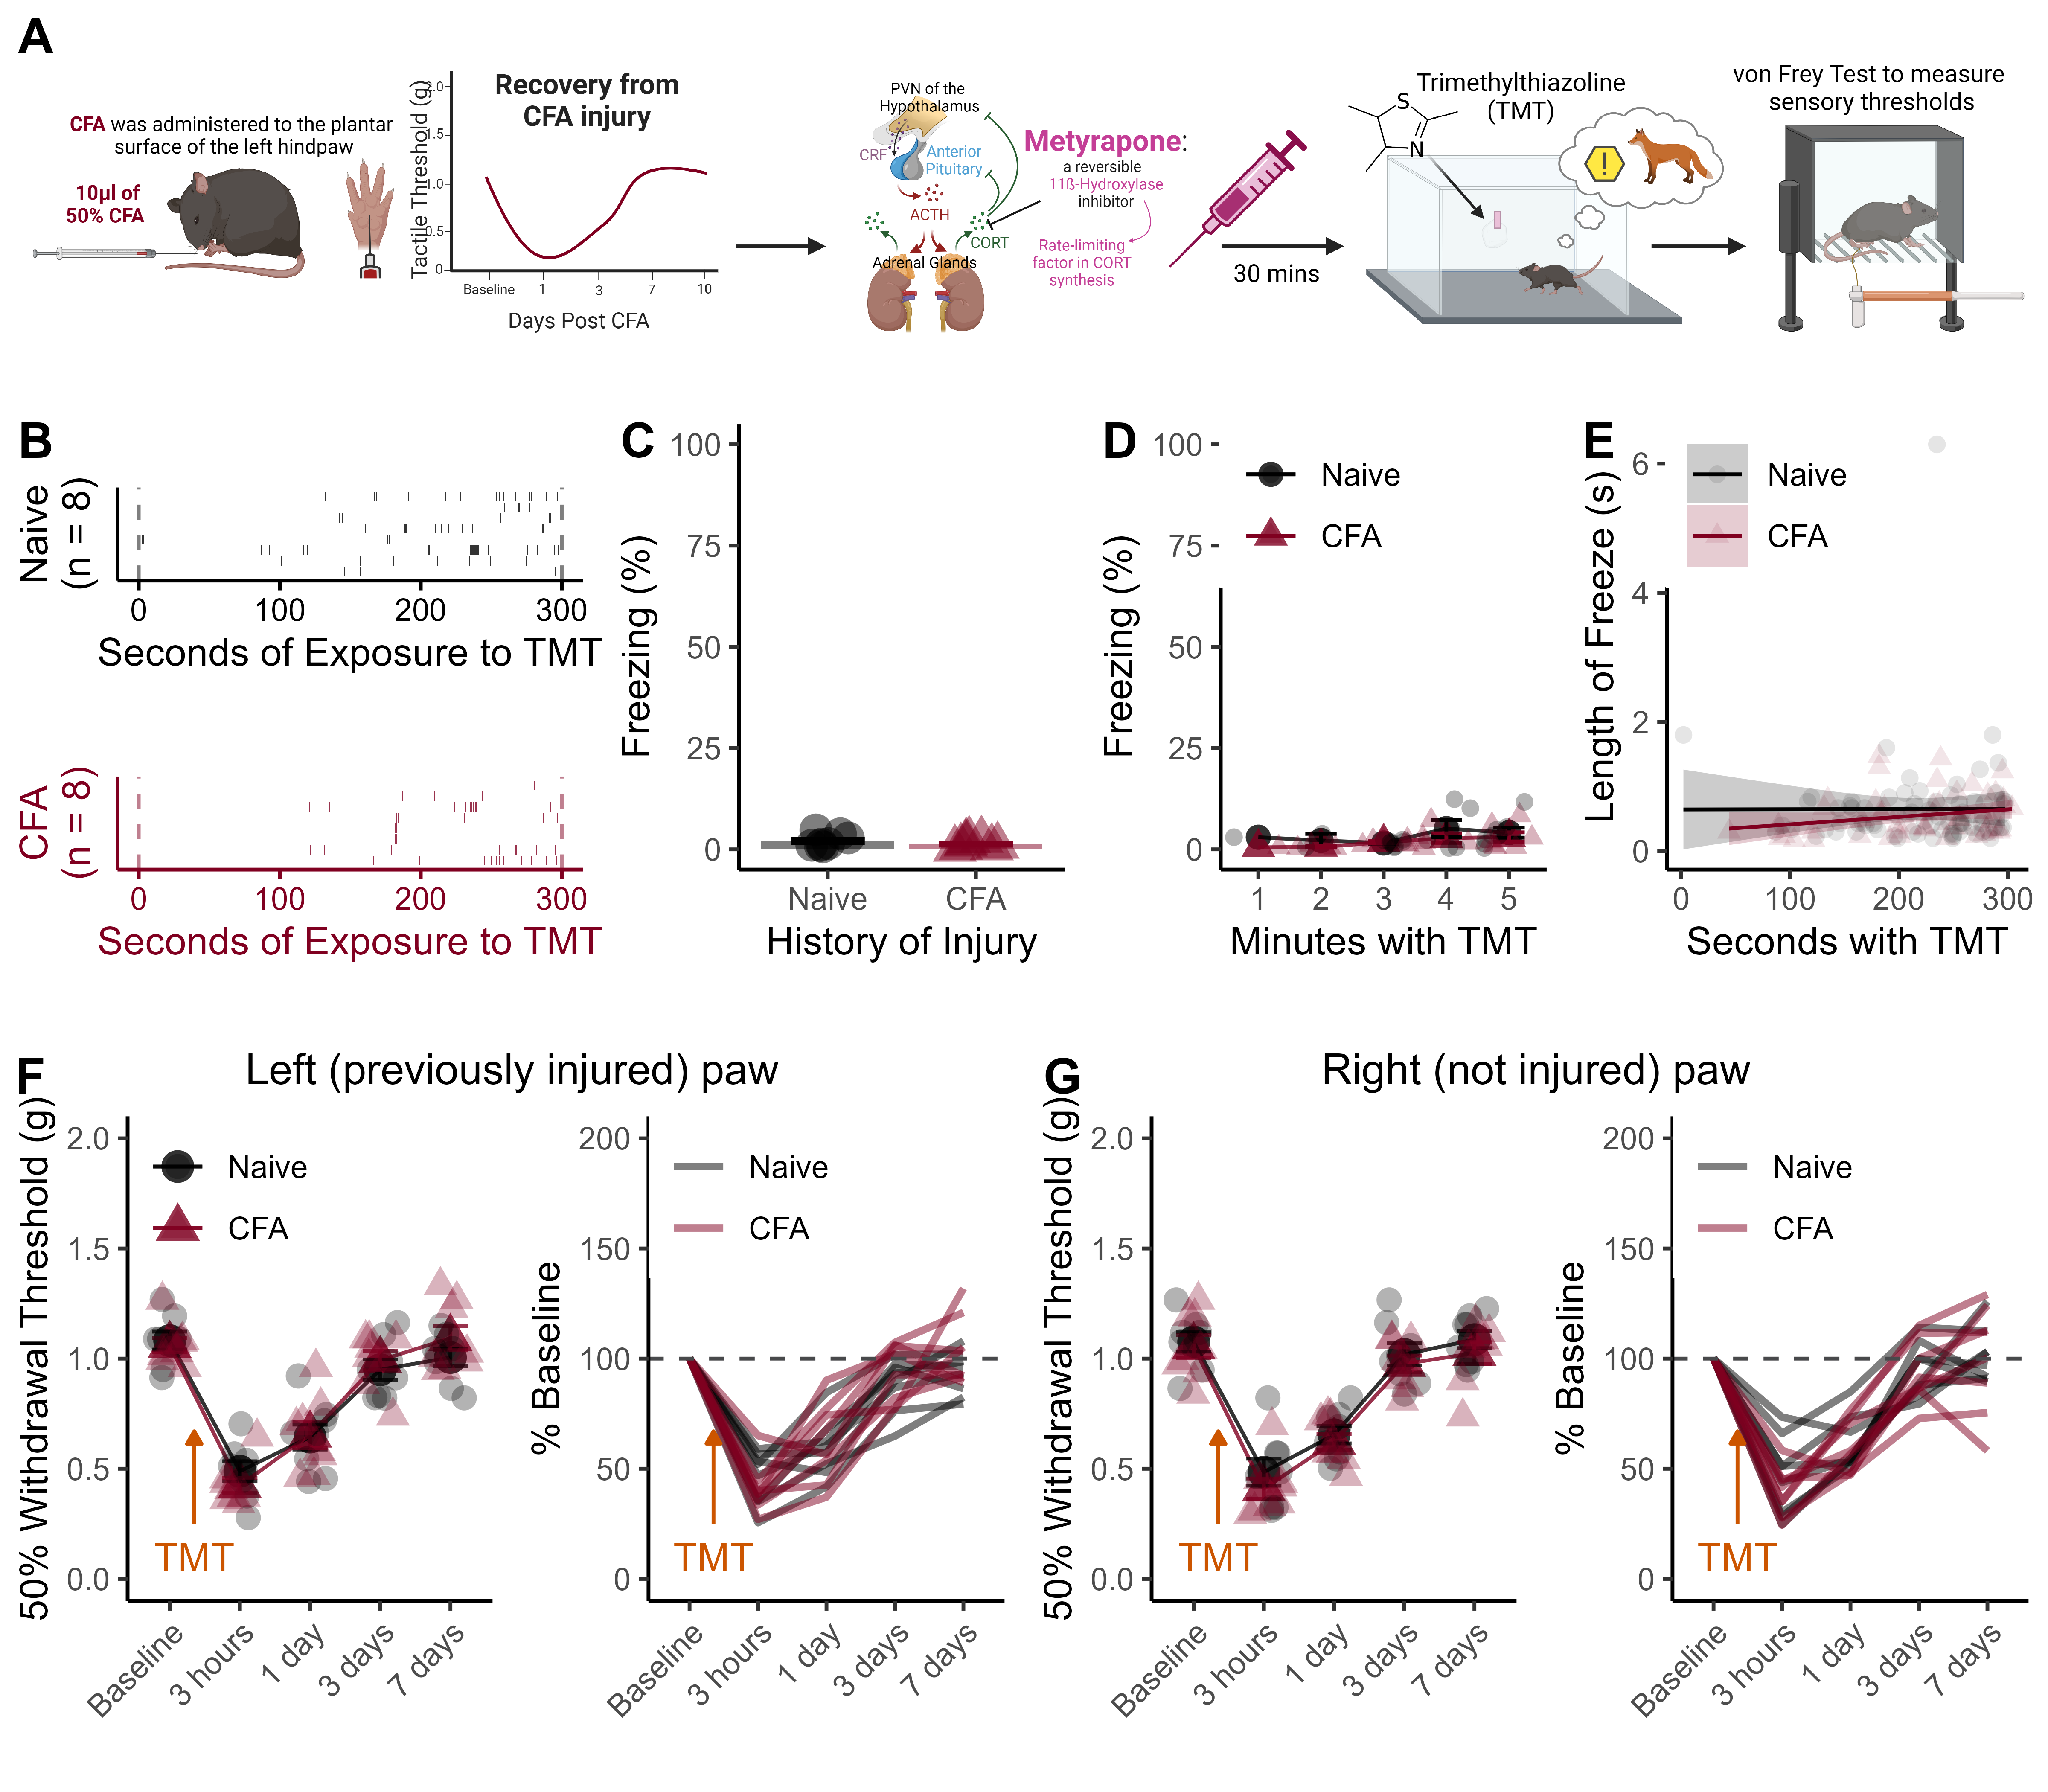
\includegraphics[width=66.67in]{Figs/4_Mety_Frz_panel}

\textbf{Figure 4. \emph{Enhanced corticosterone production during TMT mediates chronification of mechanical hypersensitivity in CFA-primed mice.}} (A) Mice were injected with CFA and given 10 days to recover. 30 minutes before a single exposure to TMT, mice were injected with the corticosterone-synthesis inhibitor metyrapone (50 mg/kg). (B) Raster plots of freezing behavior during TMT exposure for metyrapone-treated mice. (C) Metrapone blocks freezing behavior during TMT and eliminates the group difference in freezing between CFA-primed and naive mice. (D) metyrapone blocks the increase in freezing across minutes with TMT. (E) There was no increase in the length of freezing episodes across the TMT session for metyrapone-treated mice. (F) Mechanical hypersensitivity after TMT in the left hindpaws. (G) Mechanical hypersensitivity after TMT in the right hidpaws.

\section*{Time Spent Freezing Behavior During TMT}\label{time-spent-freezing-behavior-during-tmt}
\addcontentsline{toc}{section}{Time Spent Freezing Behavior During TMT}

Next, we administered the corticosterone synthesis inhibitor metyrapone to CFA-primed and pain-naive mice 30 minutes before a single five-minute TMT exposure to determine whether the hormonal stress response is necessary for TMT-induced freezing or mechanical hypersensitivity (Figure 4A).

\begin{Shaded}
\begin{Highlighting}[]
\NormalTok{b }\OtherTok{\textless{}{-}}\NormalTok{ data  }\SpecialCharTok{\%\textgreater{}\%}
  \FunctionTok{filter}\NormalTok{(Behavior }\SpecialCharTok{==} \StringTok{"freeze"}\NormalTok{) }\SpecialCharTok{\%\textgreater{}\%}
  \FunctionTok{group\_by}\NormalTok{(ID,Condition) }\SpecialCharTok{\%\textgreater{}\%}
  \FunctionTok{summarise}\NormalTok{(}
    \AttributeTok{sum=}\FunctionTok{sum}\NormalTok{(Duration),}
    \AttributeTok{Number=}\FunctionTok{n}\NormalTok{(),}
\NormalTok{  ) }\SpecialCharTok{\%\textgreater{}\%}
  \FunctionTok{mutate}\NormalTok{(}\AttributeTok{Perc =}\NormalTok{ (sum }\SpecialCharTok{/} \DecValTok{300}\NormalTok{)}\SpecialCharTok{*}\DecValTok{100}\NormalTok{) }\SpecialCharTok{\%\textgreater{}\%}
  \FunctionTok{mutate}\NormalTok{(}\AttributeTok{Av\_DUR =}\NormalTok{ (sum }\SpecialCharTok{/}\NormalTok{ Number))}
\end{Highlighting}
\end{Shaded}

\begin{verbatim}
## `summarise()` has grouped output by 'ID'. You can override using the `.groups`
## argument.
\end{verbatim}

\begin{Shaded}
\begin{Highlighting}[]
\FunctionTok{t.test}\NormalTok{(Perc}\SpecialCharTok{\textasciitilde{}}\NormalTok{Condition,}\AttributeTok{data=}\NormalTok{b,}\AttributeTok{var.equal=}\ConstantTok{TRUE}\NormalTok{)}
\end{Highlighting}
\end{Shaded}

\begin{verbatim}
## 
##  Two Sample t-test
## 
## data:  Perc by Condition
## t = 1.4134, df = 14, p-value = 0.1794
## alternative hypothesis: true difference in means between group Naive and group CFA is not equal to 0
## 95 percent confidence interval:
##  -0.4533198  2.2054031
## sample estimates:
## mean in group Naive   mean in group CFA 
##            2.092833            1.216792
\end{verbatim}

Although metryapone does not alter general locomotor behavior in an open field (Figure S4), inhibition of corticosterone synthesis prevented TMT-induced freezing (Figure 4B) and eliminated the group differences in freezing between CFA-primed and pain-naive mice (p = 0.17, Figure 4C).

\begin{Shaded}
\begin{Highlighting}[]
\NormalTok{a }\OtherTok{\textless{}{-}}\NormalTok{ data }\SpecialCharTok{\%\textgreater{}\%}
  \FunctionTok{na.omit}\NormalTok{() }\SpecialCharTok{\%\textgreater{}\%}
  \FunctionTok{mutate}\NormalTok{(}\AttributeTok{Bins =} \FunctionTok{cut}\NormalTok{(}
\NormalTok{    Start\_clean,}
    \AttributeTok{breaks =} \DecValTok{5}\NormalTok{,}
    \AttributeTok{labels=}\FunctionTok{c}\NormalTok{(}\StringTok{"1"}\NormalTok{,}\StringTok{"2"}\NormalTok{,}\StringTok{"3"}\NormalTok{,}\StringTok{"4"}\NormalTok{,}\StringTok{"5"}\NormalTok{)}
\NormalTok{  )) }\SpecialCharTok{\%\textgreater{}\%}
  \FunctionTok{group\_by}\NormalTok{(ID, Behavior, Condition, Bins) }\SpecialCharTok{\%\textgreater{}\%}
  \FunctionTok{filter}\NormalTok{(Behavior }\SpecialCharTok{==} \StringTok{"freeze"}\NormalTok{)}

\NormalTok{anova }\OtherTok{\textless{}{-}} \FunctionTok{aov}\NormalTok{(Duration}\SpecialCharTok{\textasciitilde{}}\NormalTok{Bins}\SpecialCharTok{*}\NormalTok{Condition,}\AttributeTok{data=}\NormalTok{a)}
\FunctionTok{summary}\NormalTok{(anova)}
\end{Highlighting}
\end{Shaded}

\begin{verbatim}
##                 Df Sum Sq Mean Sq F value Pr(>F)
## Bins             4   1.77  0.4415   1.234  0.300
## Condition        1   0.29  0.2934   0.820  0.367
## Bins:Condition   4   2.52  0.6291   1.758  0.142
## Residuals      120  42.93  0.3578
\end{verbatim}

Blocking the hormonal stress response also prevented the expected increase in freezing over the five-minute TMT exposure (p = 0.33, Figure 4D)

\begin{Shaded}
\begin{Highlighting}[]
\NormalTok{x }\OtherTok{\textless{}{-}}\NormalTok{ data }\SpecialCharTok{\%\textgreater{}\%}
  \FunctionTok{filter}\NormalTok{(Duration }\SpecialCharTok{\textless{}} \DecValTok{4}\NormalTok{)}

\NormalTok{b }\OtherTok{\textless{}{-}} \FunctionTok{lm}\NormalTok{(Duration}\SpecialCharTok{\textasciitilde{}}\NormalTok{Start\_clean }\SpecialCharTok{*}\NormalTok{ Condition, }\AttributeTok{data=}\NormalTok{x)}
\FunctionTok{summary}\NormalTok{(b)}
\end{Highlighting}
\end{Shaded}

\begin{verbatim}
## 
## Call:
## lm(formula = Duration ~ Start_clean * Condition, data = x)
## 
## Residuals:
##     Min      1Q  Median      3Q     Max 
## -0.9888 -0.5259 -0.1586  0.3371  2.9247 
## 
## Coefficients:
##                            Estimate Std. Error t value Pr(>|t|)    
## (Intercept)               1.0959277  0.0725218  15.112   <2e-16 ***
## Start_clean              -0.0003900  0.0004045  -0.964    0.335    
## ConditionCFA             -0.0312178  0.1054500  -0.296    0.767    
## Start_clean:ConditionCFA  0.0008662  0.0005866   1.477    0.140    
## ---
## Signif. codes:  0 '***' 0.001 '**' 0.01 '*' 0.05 '.' 0.1 ' ' 1
## 
## Residual standard error: 0.7025 on 756 degrees of freedom
## Multiple R-squared:  0.008431,   Adjusted R-squared:  0.004496 
## F-statistic: 2.143 on 3 and 756 DF,  p-value: 0.09349
\end{verbatim}

and the extension of freezing episode duration across the session (p = 0.30, Figure 4E).

\section*{Raw VF scores}\label{raw-vf-scores}
\addcontentsline{toc}{section}{Raw VF scores}

\begin{Shaded}
\begin{Highlighting}[]
\CommentTok{\# Left paws}
\NormalTok{L\_res }\OtherTok{\textless{}{-}} \FunctionTok{aov}\NormalTok{(value }\SpecialCharTok{\textasciitilde{}}\NormalTok{ variable }\SpecialCharTok{*}\NormalTok{ Condition, }\AttributeTok{data =}\NormalTok{ a)}
\FunctionTok{summary}\NormalTok{(L\_res)}
\end{Highlighting}
\end{Shaded}

\begin{verbatim}
##                    Df Sum Sq Mean Sq F value Pr(>F)    
## variable            4  4.772  1.1931  69.185 <2e-16 ***
## Condition           1  0.002  0.0025   0.145  0.705    
## variable:Condition  4  0.055  0.0137   0.794  0.533    
## Residuals          70  1.207  0.0172                   
## ---
## Signif. codes:  0 '***' 0.001 '**' 0.01 '*' 0.05 '.' 0.1 ' ' 1
\end{verbatim}

\begin{Shaded}
\begin{Highlighting}[]
\CommentTok{\# Right paws}
\NormalTok{R\_res }\OtherTok{\textless{}{-}} \FunctionTok{aov}\NormalTok{(value }\SpecialCharTok{\textasciitilde{}}\NormalTok{ variable }\SpecialCharTok{*}\NormalTok{ Condition, }\AttributeTok{data =}\NormalTok{ b)}
\FunctionTok{summary}\NormalTok{(R\_res)}
\end{Highlighting}
\end{Shaded}

\begin{verbatim}
##                    Df Sum Sq Mean Sq F value Pr(>F)    
## variable            4  5.075  1.2686  74.424 <2e-16 ***
## Condition           1  0.043  0.0433   2.540  0.116    
## variable:Condition  4  0.007  0.0019   0.109  0.979    
## Residuals          70  1.193  0.0170                   
## ---
## Signif. codes:  0 '***' 0.001 '**' 0.01 '*' 0.05 '.' 0.1 ' ' 1
\end{verbatim}

Despite the complete absence of TMT-induced freezing among metyrapone-treated mice, both CFA-primed and pain-naive mice exhibited significant bilateral mechanical hypersensitivity after TMT exposure (Left hindpaws: F4,70 = 69.18, p \textless{} 0.0001, Figure 4F; Right hindpaws: F4,70 = 74.42, p \textless{} 0.0001, Figure 4G).

\section*{VF Thresholds Relative to Baseline Measurements}\label{vf-thresholds-relative-to-baseline-measurements}
\addcontentsline{toc}{section}{VF Thresholds Relative to Baseline Measurements}

\begin{Shaded}
\begin{Highlighting}[]
\CommentTok{\# Left paws }
\NormalTok{a }\SpecialCharTok{\%\textgreater{}\%}
  \FunctionTok{group\_by}\NormalTok{(Condition) }\SpecialCharTok{\%\textgreater{}\%}
  \FunctionTok{pairwise\_t\_test}\NormalTok{(value }\SpecialCharTok{\textasciitilde{}}\NormalTok{ variable, }\AttributeTok{p.adjust.method =} \StringTok{"fdr"}\NormalTok{)}
\end{Highlighting}
\end{Shaded}

\begin{verbatim}
## # A tibble: 20 x 10
##    Condition .y.   group1 group2    n1    n2        p p.signif    p.adj
##  * <fct>     <chr> <chr>  <chr>  <int> <int>    <dbl> <chr>       <dbl>
##  1 Naive     value BL_L   L_3hr      8     8 9.95e-11 ****     9.95e-10
##  2 Naive     value BL_L   L_24hr     8     8 9.29e- 8 ****     2.32e- 7
##  3 Naive     value L_3hr  L_24hr     8     8 2.3 e- 2 *        3.29e- 2
##  4 Naive     value BL_L   L_3D       8     8 5.07e- 2 ns       6.34e- 2
##  5 Naive     value L_3hr  L_3D       8     8 3.23e- 8 ****     1.08e- 7
##  6 Naive     value L_24hr L_3D       8     8 4.22e- 5 ****     7.03e- 5
##  7 Naive     value BL_L   L_7D       8     8 2.49e- 1 ns       2.77e- 1
##  8 Naive     value L_3hr  L_7D       8     8 2.68e- 9 ****     1.34e- 8
##  9 Naive     value L_24hr L_7D       8     8 3.22e- 6 ****     6.44e- 6
## 10 Naive     value L_3D   L_7D       8     8 4.01e- 1 ns       4.01e- 1
## 11 CFA       value BL_L   L_3hr      8     8 2.08e-11 ****     1.04e-10
## 12 CFA       value BL_L   L_24hr     8     8 4.62e- 7 ****     9.24e- 7
## 13 CFA       value L_3hr  L_24hr     8     8 1.32e- 3 **       1.89e- 3
## 14 CFA       value BL_L   L_3D       8     8 3.03e- 1 ns       3.37e- 1
## 15 CFA       value L_3hr  L_3D       8     8 3.61e-10 ****     1.20e- 9
## 16 CFA       value L_24hr L_3D       8     8 1.10e- 5 ****     1.84e- 5
## 17 CFA       value BL_L   L_7D       8     8 6.32e- 1 ns       6.32e- 1
## 18 CFA       value L_3hr  L_7D       8     8 5.83e-12 ****     5.83e-11
## 19 CFA       value L_24hr L_7D       8     8 1.08e- 7 ****     2.69e- 7
## 20 CFA       value L_3D   L_7D       8     8 1.35e- 1 ns       1.69e- 1
## # i 1 more variable: p.adj.signif <chr>
\end{verbatim}

\begin{Shaded}
\begin{Highlighting}[]
\CommentTok{\# Right paws}
\NormalTok{b }\SpecialCharTok{\%\textgreater{}\%}
  \FunctionTok{group\_by}\NormalTok{(Condition) }\SpecialCharTok{\%\textgreater{}\%}
  \FunctionTok{pairwise\_t\_test}\NormalTok{(value }\SpecialCharTok{\textasciitilde{}}\NormalTok{ variable, }\AttributeTok{p.adjust.method =} \StringTok{"fdr"}\NormalTok{)}
\end{Highlighting}
\end{Shaded}

\begin{verbatim}
## # A tibble: 20 x 10
##    Condition .y.   group1 group2    n1    n2        p p.signif    p.adj
##  * <fct>     <chr> <chr>  <chr>  <int> <int>    <dbl> <chr>       <dbl>
##  1 Naive     value BL_R   R_3hr      8     8 2.06e-10 ****     1.03e- 9
##  2 Naive     value BL_R   R_24hr     8     8 3.28e- 7 ****     6.56e- 7
##  3 Naive     value R_3hr  R_24hr     8     8 1.59e- 2 *        2.28e- 2
##  4 Naive     value BL_R   R_3D       8     8 4.04e- 1 ns       4.48e- 1
##  5 Naive     value R_3hr  R_3D       8     8 2.24e- 9 ****     7.45e- 9
##  6 Naive     value R_24hr R_3D       8     8 4.27e- 6 ****     7.11e- 6
##  7 Naive     value BL_R   R_7D       8     8 8.78e- 1 ns       8.78e- 1
##  8 Naive     value R_3hr  R_7D       8     8 1.34e-10 ****     1.03e- 9
##  9 Naive     value R_24hr R_7D       8     8 2.06e- 7 ****     5.14e- 7
## 10 Naive     value R_3D   R_7D       8     8 3.24e- 1 ns       4.05e- 1
## 11 CFA       value BL_R   R_3hr      8     8 5.49e-12 ****     5.49e-11
## 12 CFA       value BL_R   R_24hr     8     8 6.60e- 8 ****     1.65e- 7
## 13 CFA       value R_3hr  R_24hr     8     8 1.94e- 3 **       2.78e- 3
## 14 CFA       value BL_R   R_3D       8     8 2.22e- 1 ns       2.78e- 1
## 15 CFA       value R_3hr  R_3D       8     8 1.53e-10 ****     5.09e-10
## 16 CFA       value R_24hr R_3D       8     8 2.82e- 6 ****     4.70e- 6
## 17 CFA       value BL_R   R_7D       8     8 6.49e- 1 ns       6.49e- 1
## 18 CFA       value R_3hr  R_7D       8     8 1.83e-11 ****     9.17e-11
## 19 CFA       value R_24hr R_7D       8     8 2.62e- 7 ****     5.25e- 7
## 20 CFA       value R_3D   R_7D       8     8 4.39e- 1 ns       4.87e- 1
## # i 1 more variable: p.adj.signif <chr>
\end{verbatim}

CFA-primed mice showed resolution of TMT-induced mechanical hypersensitivity within one week post-exposure (naive: both paws p \textgreater{} 0.27 relative to baseline measurements; CFA-primed: both paws p \textgreater{} 0.63), suggesting that the exaggerated hormonal stress response during TMT modulates the persistence of TMT-evoked mechanical hypersensitivity among mice with a history of CFA injury.

\chapter*{Figure 5}\label{figure-5}
\addcontentsline{toc}{chapter}{Figure 5}

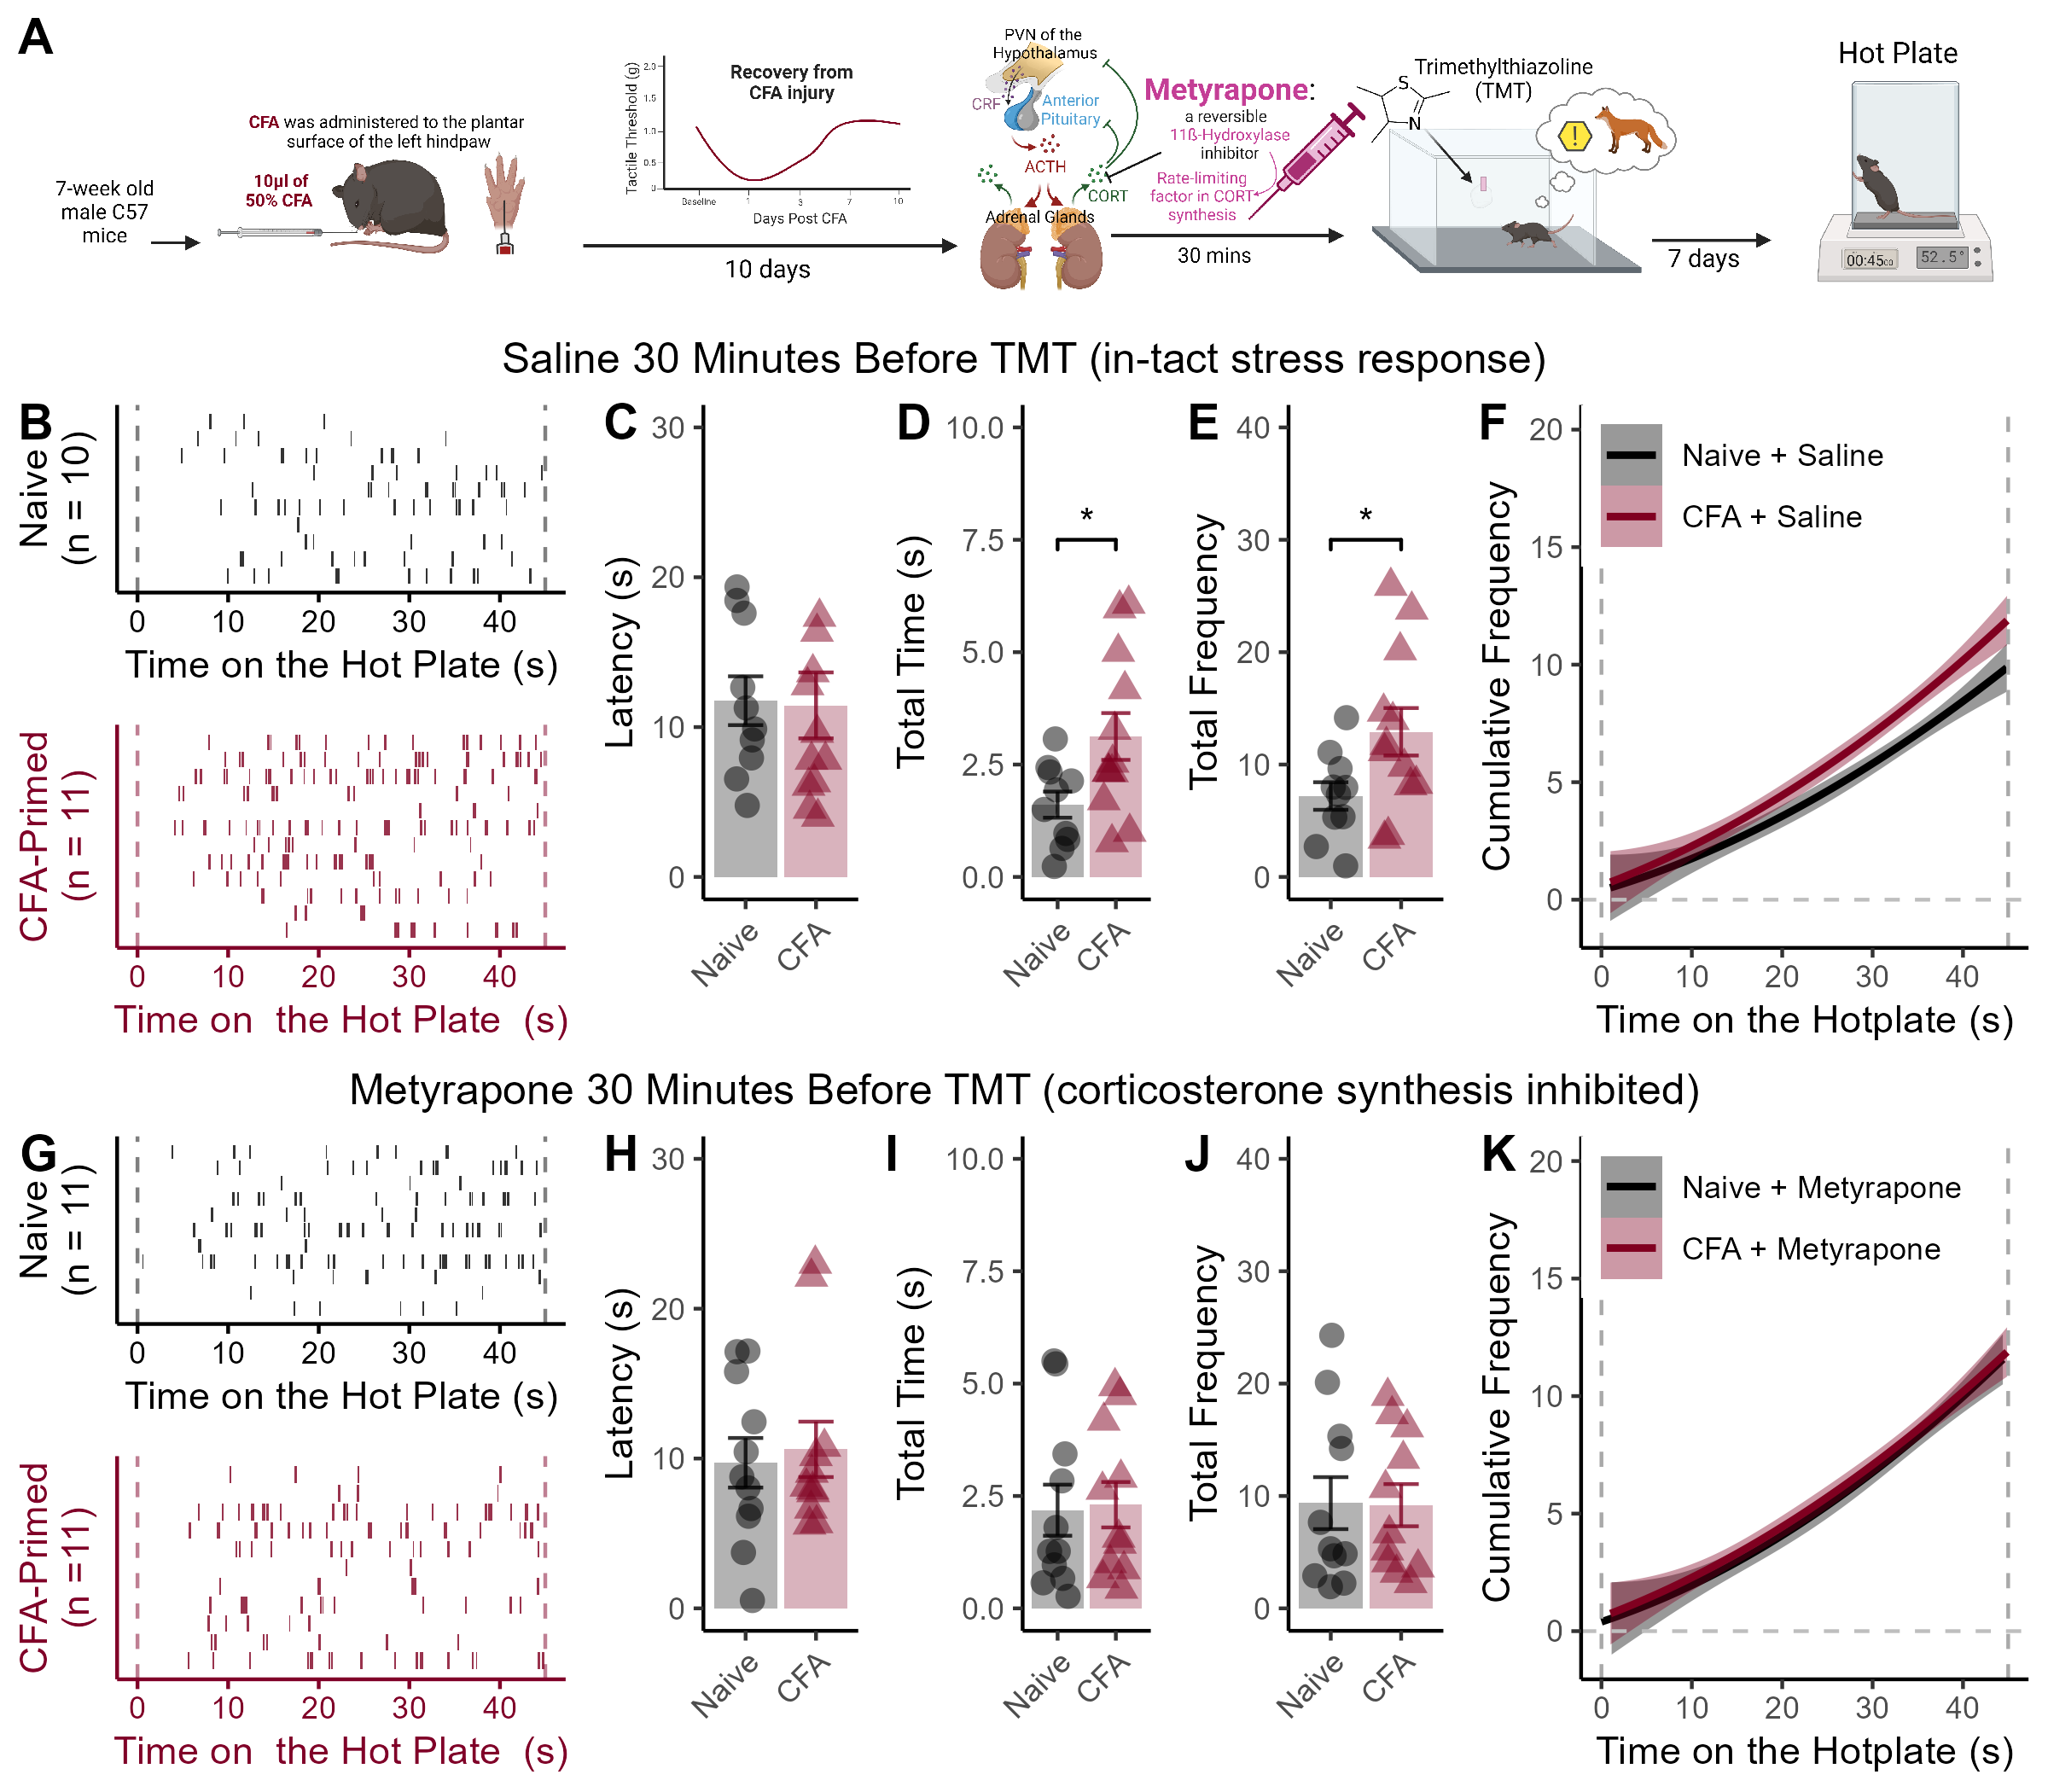
\includegraphics[width=33.33in]{Figs/5_HP_Mety}

\textbf{Figure 5. \emph{Enhanced corticosterone production during TMT facilitates nociceptive responses on the hotplate among CFA-primed mice.}} (A) Timeline of experimental procedures. Mice were administered CFA and allowed 10 days to recover. Thirty minutes before a single exposure to TMT, mice were injected (i.p.) with 50 mg / kg metyrapone or Saline control. One week after the single exposure to TMT nociceptive responses during a 45-second exposure to a 52.5-degree hotplate were measured. (B) Raster plots of nociceptive responses during the hotplate test for saline-treated mice. (C) Latency to exhibit the first nociceptive response during testing. (D) CFA-primed mice spent more time exhibiting nociceptive responses, and (E) exhibited a higher frequency of nociceptive responses. (F) The cumulative frequency of nociceptive responses across the session. (G) Raster plots of nociceptive responses across the hotplate test for metyrapone-injected mice. (H) Latency to exhibit the first nociceptive response during the hotplate test. (I) Metraypone injection blocks the enhancing effect of CFA-priming on time spent exhibiting nociceptive behaviors on the hotplate, and (J) the frequency of nociceptive responses during the task. (K) Cumulative frequency of nociceptive responses for metyrapone-treated mice. Data displayed as mean value +/- SEM. * indicates \emph{p} \textless{} 0.05.

\section*{Effect of CFA for Saline-Treated Mice}\label{effect-of-cfa-for-saline-treated-mice}
\addcontentsline{toc}{section}{Effect of CFA for Saline-Treated Mice}

\begin{Shaded}
\begin{Highlighting}[]
\NormalTok{a }\OtherTok{\textless{}{-}}\NormalTok{ LE\_data }\SpecialCharTok{\%\textgreater{}\%}
  \FunctionTok{group\_by}\NormalTok{(ID,CFA) }\SpecialCharTok{\%\textgreater{}\%}
  \FunctionTok{filter}\NormalTok{(Behavior }\SpecialCharTok{==} \StringTok{"shake/flick"}\NormalTok{) }\SpecialCharTok{\%\textgreater{}\%}
  \FunctionTok{filter}\NormalTok{(Drug }\SpecialCharTok{==} \StringTok{"Saline"}\NormalTok{) }\SpecialCharTok{\%\textgreater{}\%}
  \FunctionTok{summarise}\NormalTok{(}
    \AttributeTok{min=}\FunctionTok{min}\NormalTok{(Start\_clean)}
\NormalTok{  )}
\end{Highlighting}
\end{Shaded}

\begin{verbatim}
## `summarise()` has grouped output by 'ID'. You can override using the `.groups`
## argument.
\end{verbatim}

\begin{Shaded}
\begin{Highlighting}[]
\FunctionTok{t.test}\NormalTok{(}\AttributeTok{data =}\NormalTok{ a, min }\SpecialCharTok{\textasciitilde{}}\NormalTok{ CFA, }\AttributeTok{var.equal =}\NormalTok{ T)}
\end{Highlighting}
\end{Shaded}

\begin{verbatim}
## 
##  Two Sample t-test
## 
## data:  min by CFA
## t = 0.11032, df = 20, p-value = 0.9133
## alternative hypothesis: true difference in means between group Naive and group CFA is not equal to 0
## 95 percent confidence interval:
##  -5.606881  6.233048
## sample estimates:
## mean in group Naive   mean in group CFA 
##            11.76050            11.44742
\end{verbatim}

We also investigated whether metyrapone administration prior to TMT exposure would alter nociceptive behaviors on the hotplate in CFA-primed mice. One week after a single TMT exposure, mice were tested on a 52.5 degree hotplate for 45 seconds (Figure 5A). Although there was no group difference in latency to the first nociceptive response (p = 0.91, Figure 5B, C),

\begin{Shaded}
\begin{Highlighting}[]
\NormalTok{data }\OtherTok{\textless{}{-}}\NormalTok{ LE\_data }\SpecialCharTok{\%\textgreater{}\%}
  \FunctionTok{filter}\NormalTok{(Behavior }\SpecialCharTok{==} \StringTok{"shake/flick"}\NormalTok{) }

\DocumentationTok{\#\# Saline{-}treated}
\NormalTok{saline }\OtherTok{\textless{}{-}}\NormalTok{ data }\SpecialCharTok{\%\textgreater{}\%} 
  \FunctionTok{filter}\NormalTok{(Drug }\SpecialCharTok{==} \StringTok{"Saline"}\NormalTok{)}

\NormalTok{a }\OtherTok{\textless{}{-}}\NormalTok{ saline }\SpecialCharTok{\%\textgreater{}\%}
  \FunctionTok{group\_by}\NormalTok{(ID,CFA) }\SpecialCharTok{\%\textgreater{}\%}
  \FunctionTok{summarize}\NormalTok{(}
    \AttributeTok{sum=}\FunctionTok{sum}\NormalTok{(Duration)}
\NormalTok{  )}
\end{Highlighting}
\end{Shaded}

\begin{verbatim}
## `summarise()` has grouped output by 'ID'. You can override using the `.groups`
## argument.
\end{verbatim}

\begin{Shaded}
\begin{Highlighting}[]
\FunctionTok{t.test}\NormalTok{(sum }\SpecialCharTok{\textasciitilde{}}\NormalTok{ CFA, }\AttributeTok{data =}\NormalTok{ a, }\AttributeTok{var.equal =}\NormalTok{ T)}
\end{Highlighting}
\end{Shaded}

\begin{verbatim}
## 
##  Two Sample t-test
## 
## data:  sum by CFA
## t = -2.4052, df = 20, p-value = 0.02596
## alternative hypothesis: true difference in means between group Naive and group CFA is not equal to 0
## 95 percent confidence interval:
##  -2.8316628 -0.2013039
## sample estimates:
## mean in group Naive   mean in group CFA 
##            1.608100            3.124583
\end{verbatim}

CFA-primed mice that were administered a saline vehicle 30 minutes before TMT spent more time exhibiting nociceptive responses on the hotplate (t20 = 2.4, p = 0.026, Figure 5D),

\begin{Shaded}
\begin{Highlighting}[]
\NormalTok{a }\OtherTok{\textless{}{-}}\NormalTok{ saline }\SpecialCharTok{\%\textgreater{}\%}
  \FunctionTok{group\_by}\NormalTok{(ID,CFA) }\SpecialCharTok{\%\textgreater{}\%}
  \FunctionTok{summarise}\NormalTok{(}
    \AttributeTok{n=}\FunctionTok{n}\NormalTok{()}
\NormalTok{  )}
\end{Highlighting}
\end{Shaded}

\begin{verbatim}
## `summarise()` has grouped output by 'ID'. You can override using the `.groups`
## argument.
\end{verbatim}

\begin{Shaded}
\begin{Highlighting}[]
\FunctionTok{t.test}\NormalTok{(n }\SpecialCharTok{\textasciitilde{}}\NormalTok{ CFA, }\AttributeTok{data =}\NormalTok{ a, }\AttributeTok{var.equal =}\NormalTok{ T)}
\end{Highlighting}
\end{Shaded}

\begin{verbatim}
## 
##  Two Sample t-test
## 
## data:  n by CFA
## t = -2.2183, df = 20, p-value = 0.03828
## alternative hypothesis: true difference in means between group Naive and group CFA is not equal to 0
## 95 percent confidence interval:
##  -11.0923862  -0.3409471
## sample estimates:
## mean in group Naive   mean in group CFA 
##             7.20000            12.91667
\end{verbatim}

and a higher frequency of nociceptive responses (t20 = 2.22, p = 0.038, Figure 5E, F).

\section*{No Effect of CFA for Metyrapone-Treated Mice}\label{no-effect-of-cfa-for-metyrapone-treated-mice}
\addcontentsline{toc}{section}{No Effect of CFA for Metyrapone-Treated Mice}

\begin{Shaded}
\begin{Highlighting}[]
\NormalTok{mety }\OtherTok{\textless{}{-}}\NormalTok{ data }\SpecialCharTok{\%\textgreater{}\%}
  \FunctionTok{filter}\NormalTok{(Drug }\SpecialCharTok{==} \StringTok{"Metyrapone"}\NormalTok{)}

\NormalTok{a }\OtherTok{\textless{}{-}}\NormalTok{ mety }\SpecialCharTok{\%\textgreater{}\%}
  \FunctionTok{group\_by}\NormalTok{(ID,CFA) }\SpecialCharTok{\%\textgreater{}\%}
  \FunctionTok{summarize}\NormalTok{(}
    \AttributeTok{sum=}\FunctionTok{sum}\NormalTok{(Duration)}
\NormalTok{  )}
\end{Highlighting}
\end{Shaded}

\begin{verbatim}
## `summarise()` has grouped output by 'ID'. You can override using the `.groups`
## argument.
\end{verbatim}

\begin{Shaded}
\begin{Highlighting}[]
\FunctionTok{t.test}\NormalTok{(sum }\SpecialCharTok{\textasciitilde{}}\NormalTok{ CFA, }\AttributeTok{data =}\NormalTok{ a, }\AttributeTok{var.equal =}\NormalTok{ T)}
\end{Highlighting}
\end{Shaded}

\begin{verbatim}
## 
##  Two Sample t-test
## 
## data:  sum by CFA
## t = -0.15991, df = 20, p-value = 0.8746
## alternative hypothesis: true difference in means between group Naive and group CFA is not equal to 0
## 95 percent confidence interval:
##  -1.707064  1.463973
## sample estimates:
## mean in group Naive   mean in group CFA 
##            2.183727            2.305273
\end{verbatim}

\begin{Shaded}
\begin{Highlighting}[]
\NormalTok{a }\OtherTok{\textless{}{-}}\NormalTok{ mety }\SpecialCharTok{\%\textgreater{}\%}
  \FunctionTok{group\_by}\NormalTok{(ID,CFA) }\SpecialCharTok{\%\textgreater{}\%}
  \FunctionTok{summarise}\NormalTok{(}
    \AttributeTok{n=}\FunctionTok{n}\NormalTok{()}
\NormalTok{  )}
\end{Highlighting}
\end{Shaded}

\begin{verbatim}
## `summarise()` has grouped output by 'ID'. You can override using the `.groups`
## argument.
\end{verbatim}

\begin{Shaded}
\begin{Highlighting}[]
\FunctionTok{t.test}\NormalTok{(n }\SpecialCharTok{\textasciitilde{}}\NormalTok{ CFA, }\AttributeTok{data =}\NormalTok{ a, }\AttributeTok{var.equal =}\NormalTok{ T)}
\end{Highlighting}
\end{Shaded}

\begin{verbatim}
## 
##  Two Sample t-test
## 
## data:  n by CFA
## t = 0.061034, df = 20, p-value = 0.9519
## alternative hypothesis: true difference in means between group Naive and group CFA is not equal to 0
## 95 percent confidence interval:
##  -6.032246  6.395882
## sample estimates:
## mean in group Naive   mean in group CFA 
##            9.363636            9.181818
\end{verbatim}

In contrast, no group differences in hotplate behavior were observed between CFA-primed and pain-naive mice treated with metyrapone prior to TMT exposure (all p \textgreater{} 0.87, Figure 5G-K).

\chapter*{Figure 6}\label{figure-6}
\addcontentsline{toc}{chapter}{Figure 6}

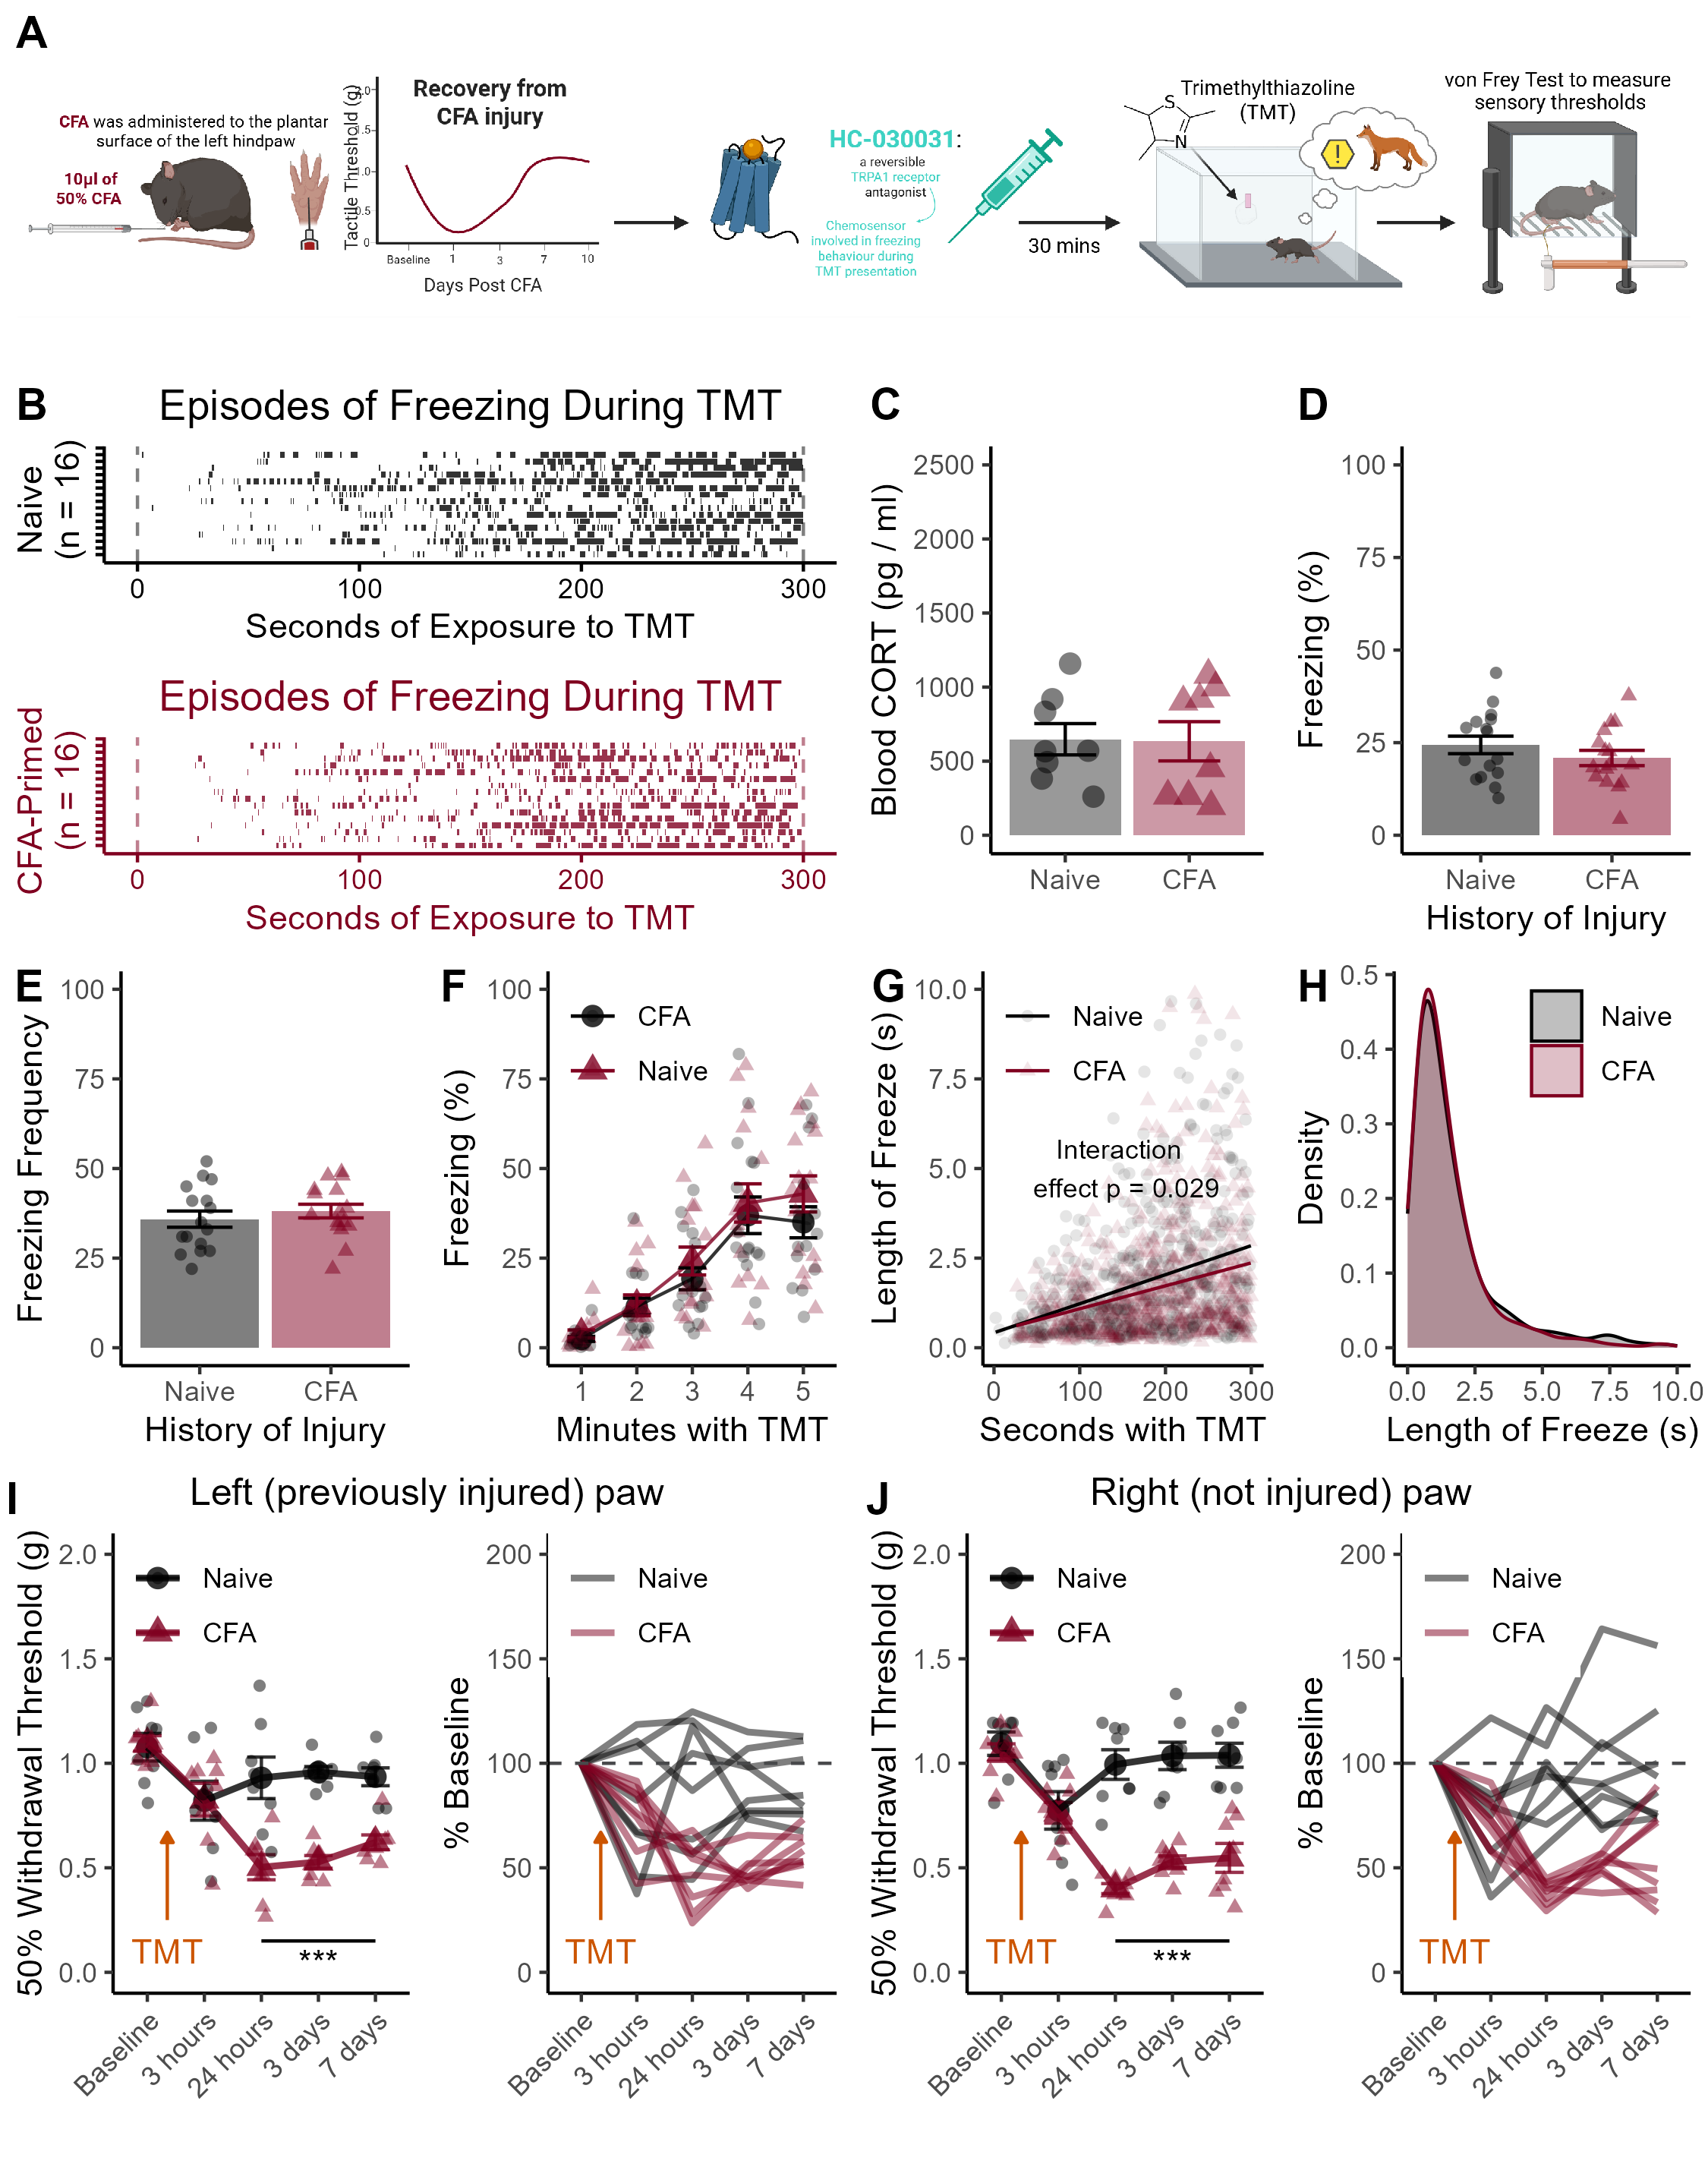
\includegraphics[width=31.25in]{Figs/6_HC30031_panel}

\textbf{Figure 6. \emph{Sensitization of TRPA1 signaling regulates enhanced circulating corticosterone and freezing during TMT among CFA-primed mice.}} (A) Timeline of experimental procedures. Mice were injected with CFA and given 10 days to recover. Thirty minutes before a single TMT exposure, mice were injected with the TRPA-1 antagonist HC30031. (B) Raster plots of freezing behavior across the TMT session. (C) TRPA-1 antagonism normalizes circulating levels of corticosterone between pain-naive and CFA-primed mice. (D) TRPA-1 antagonism also normalizes levels of freezing during TMT exposure for CFA-primed mice. (E) Blockade of TRPA-1 signalling does not prevent the increase in freezing across the session. (F) Linear relationships between time spent with TMT and length of freezing episodes. (G) Density plots showing that TRPA-1 antagonism normalized the difference in length for freezing bouts. (H) Sensory responses after TMT in the left hind paws. (I) Sensory responses after TMT in the right hind paws. Data displayed as mean +/- SEM. *** indicates \emph{p} \textless{} 0.001.

We administered the TRPA1 receptor antagonist HC30031 (30 mg/kg, i.p.) to CFA-primed and pain-naive mice 30 minutes before a single five-minute TMT exposure (Figure 6A). TRPA1 antagonism did not prevent TMT-induced freezing behavior (Figure 6B); mice still spent significantly more time freezing during the TMT session compared to a baseline session without TMT (t31 = 13.18 , p \textless{} 0.001; data not shown).

\section*{Blood CORT Levels}\label{blood-cort-levels}
\addcontentsline{toc}{section}{Blood CORT Levels}

\begin{Shaded}
\begin{Highlighting}[]
\NormalTok{a }\OtherTok{\textless{}{-}}\NormalTok{ CORT\_data }\SpecialCharTok{\%\textgreater{}\%}
  \FunctionTok{filter}\NormalTok{(Drug }\SpecialCharTok{==} \StringTok{"HC30031"}\NormalTok{) }

\FunctionTok{t.test}\NormalTok{(}\AttributeTok{data =}\NormalTok{ a, CORT }\SpecialCharTok{\textasciitilde{}}\NormalTok{ Pain, }\AttributeTok{var.equal =} \ConstantTok{TRUE}\NormalTok{)}
\end{Highlighting}
\end{Shaded}

\begin{verbatim}
## 
##  Two Sample t-test
## 
## data:  CORT by Pain
## t = 0.081537, df = 14, p-value = 0.9362
## alternative hypothesis: true difference in means between group Naive and group CFA is not equal to 0
## 95 percent confidence interval:
##  -349.6575  377.2933
## sample estimates:
## mean in group Naive   mean in group CFA 
##            648.0151            634.1972
\end{verbatim}

However, blocking TRPA1 receptors during TMT exposure occluded enhanced corticosterone release (p = 0.93; Figure 6C).

\section*{Percent Freezing During TMT}\label{percent-freezing-during-tmt}
\addcontentsline{toc}{section}{Percent Freezing During TMT}

\begin{Shaded}
\begin{Highlighting}[]
\NormalTok{b }\OtherTok{\textless{}{-}}\NormalTok{ data  }\SpecialCharTok{\%\textgreater{}\%}
  \FunctionTok{filter}\NormalTok{(Behavior }\SpecialCharTok{==} \StringTok{"freeze"}\NormalTok{) }\SpecialCharTok{\%\textgreater{}\%}
  \FunctionTok{group\_by}\NormalTok{(ID,Condition) }\SpecialCharTok{\%\textgreater{}\%}
  \FunctionTok{summarise}\NormalTok{(}
    \AttributeTok{sum=}\FunctionTok{sum}\NormalTok{(Duration),}
    \AttributeTok{Number=}\FunctionTok{n}\NormalTok{(),}
\NormalTok{  ) }\SpecialCharTok{\%\textgreater{}\%}
  \FunctionTok{mutate}\NormalTok{(}\AttributeTok{Perc =}\NormalTok{ (sum }\SpecialCharTok{/} \DecValTok{300}\NormalTok{)}\SpecialCharTok{*}\DecValTok{100}\NormalTok{) }\SpecialCharTok{\%\textgreater{}\%}
  \FunctionTok{mutate}\NormalTok{(}\AttributeTok{Av\_DUR =}\NormalTok{ (sum }\SpecialCharTok{/}\NormalTok{ Number)) }
\end{Highlighting}
\end{Shaded}

\begin{verbatim}
## `summarise()` has grouped output by 'ID'. You can override using the `.groups`
## argument.
\end{verbatim}

\begin{Shaded}
\begin{Highlighting}[]
\FunctionTok{t.test}\NormalTok{(Perc}\SpecialCharTok{\textasciitilde{}}\NormalTok{Condition,}\AttributeTok{data=}\NormalTok{b,}\AttributeTok{var.equal=}\ConstantTok{TRUE}\NormalTok{)}
\end{Highlighting}
\end{Shaded}

\begin{verbatim}
## 
##  Two Sample t-test
## 
## data:  Perc by Condition
## t = 1.1266, df = 30, p-value = 0.2688
## alternative hypothesis: true difference in means between group Naive and group CFA is not equal to 0
## 95 percent confidence interval:
##  -2.872619  9.941494
## sample estimates:
## mean in group Naive   mean in group CFA 
##            24.38940            20.85496
\end{verbatim}

HC30031 treatment also prevented exaggerated freezing behavior for CFA-primed mice (p = 0.27; Figure 6D)

\section*{Freezing Frequency During TMT}\label{freezing-frequency-during-tmt}
\addcontentsline{toc}{section}{Freezing Frequency During TMT}

\begin{Shaded}
\begin{Highlighting}[]
\NormalTok{b }\OtherTok{\textless{}{-}}\NormalTok{ data  }\SpecialCharTok{\%\textgreater{}\%}
  \FunctionTok{filter}\NormalTok{(Behavior }\SpecialCharTok{==} \StringTok{"freeze"}\NormalTok{) }\SpecialCharTok{\%\textgreater{}\%}
  \FunctionTok{group\_by}\NormalTok{(ID,Condition) }\SpecialCharTok{\%\textgreater{}\%}
  \FunctionTok{summarise}\NormalTok{(}
    \AttributeTok{sum=}\FunctionTok{sum}\NormalTok{(Duration),}
    \AttributeTok{Number=}\FunctionTok{n}\NormalTok{(),}
\NormalTok{  ) }
\end{Highlighting}
\end{Shaded}

\begin{verbatim}
## `summarise()` has grouped output by 'ID'. You can override using the `.groups`
## argument.
\end{verbatim}

\begin{Shaded}
\begin{Highlighting}[]
\FunctionTok{t.test}\NormalTok{(Number}\SpecialCharTok{\textasciitilde{}}\NormalTok{Condition,}\AttributeTok{data=}\NormalTok{b,}\AttributeTok{var.equal=}\ConstantTok{TRUE}\NormalTok{)}
\end{Highlighting}
\end{Shaded}

\begin{verbatim}
## 
##  Two Sample t-test
## 
## data:  Number by Condition
## t = -0.76073, df = 30, p-value = 0.4528
## alternative hypothesis: true difference in means between group Naive and group CFA is not equal to 0
## 95 percent confidence interval:
##  -8.290404  3.790404
## sample estimates:
## mean in group Naive   mean in group CFA 
##              35.875              38.125
\end{verbatim}

and normalized the number of freezing episodes (p = 0.45, Figure 6E).

\section*{Freezing During Each Minute of TMT}\label{freezing-during-each-minute-of-tmt}
\addcontentsline{toc}{section}{Freezing During Each Minute of TMT}

\begin{Shaded}
\begin{Highlighting}[]
\CommentTok{\# \% Freezing each minute}
\NormalTok{a }\OtherTok{\textless{}{-}}\NormalTok{ data }\SpecialCharTok{\%\textgreater{}\%}
  \FunctionTok{na.omit}\NormalTok{() }\SpecialCharTok{\%\textgreater{}\%}
  \FunctionTok{mutate}\NormalTok{(}\AttributeTok{Bins =} \FunctionTok{cut}\NormalTok{(}
\NormalTok{    Start\_clean,}
    \AttributeTok{breaks =} \DecValTok{5}\NormalTok{,}
    \AttributeTok{labels=}\FunctionTok{c}\NormalTok{(}\StringTok{"1"}\NormalTok{,}\StringTok{"2"}\NormalTok{,}\StringTok{"3"}\NormalTok{,}\StringTok{"4"}\NormalTok{,}\StringTok{"5"}\NormalTok{)}
\NormalTok{  )) }\SpecialCharTok{\%\textgreater{}\%}
  \FunctionTok{group\_by}\NormalTok{(ID, Behavior,Condition, Bins) }\SpecialCharTok{\%\textgreater{}\%}
  \FunctionTok{summarise}\NormalTok{(}
    \AttributeTok{sum =} \FunctionTok{sum}\NormalTok{ (Duration)}
\NormalTok{  ) }\SpecialCharTok{\%\textgreater{}\%}
  \FunctionTok{mutate}\NormalTok{(}\AttributeTok{Perc =}\NormalTok{ (sum }\SpecialCharTok{/} \DecValTok{60}\NormalTok{)}\SpecialCharTok{*}\DecValTok{100}\NormalTok{ ) }\SpecialCharTok{\%\textgreater{}\%}
  \FunctionTok{filter}\NormalTok{(Behavior }\SpecialCharTok{==} \StringTok{"freeze"}\NormalTok{)}
\end{Highlighting}
\end{Shaded}

\begin{verbatim}
## `summarise()` has grouped output by 'ID', 'Behavior', 'Condition'. You can
## override using the `.groups` argument.
\end{verbatim}

\begin{Shaded}
\begin{Highlighting}[]
\NormalTok{anova }\OtherTok{\textless{}{-}} \FunctionTok{aov}\NormalTok{(Perc}\SpecialCharTok{\textasciitilde{}}\NormalTok{Bins}\SpecialCharTok{*}\NormalTok{Condition,}\AttributeTok{data=}\NormalTok{a)}
\FunctionTok{summary}\NormalTok{(anova)}
\end{Highlighting}
\end{Shaded}

\begin{verbatim}
##                 Df Sum Sq Mean Sq F value Pr(>F)    
## Bins             4  31345    7836  34.633 <2e-16 ***
## Condition        1    527     527   2.331  0.129    
## Bins:Condition   4    279      70   0.308  0.872    
## Residuals      145  32808     226                   
## ---
## Signif. codes:  0 '***' 0.001 '**' 0.01 '*' 0.05 '.' 0.1 ' ' 1
\end{verbatim}

HC30031-treated mice exhibited a clear increase in time spent freezing across the five-minute exposure (F4,145 = 34.63, p \textless{} 0.001), which was not different for CFA-primed and pain-naive mice (p = 0.12, Figure 6F).

\section*{Linear Relationship Between Time and Length of Freeze}\label{linear-relationship-between-time-and-length-of-freeze}
\addcontentsline{toc}{section}{Linear Relationship Between Time and Length of Freeze}

\begin{Shaded}
\begin{Highlighting}[]
\NormalTok{b }\OtherTok{\textless{}{-}} \FunctionTok{lm}\NormalTok{(Duration}\SpecialCharTok{\textasciitilde{}}\NormalTok{Start\_clean }\SpecialCharTok{*}\NormalTok{ Condition, }\AttributeTok{data=}\NormalTok{data)}
\FunctionTok{summary}\NormalTok{(b)}
\end{Highlighting}
\end{Shaded}

\begin{verbatim}
## 
## Call:
## lm(formula = Duration ~ Start_clean * Condition, data = data)
## 
## Residuals:
##     Min      1Q  Median      3Q     Max 
## -2.1919 -1.0243 -0.5237  0.2493 21.3420 
## 
## Coefficients:
##                            Estimate Std. Error t value Pr(>|t|)    
## (Intercept)               1.1074246  0.1251720   8.847  < 2e-16 ***
## Start_clean               0.0048383  0.0007297   6.630 4.28e-11 ***
## ConditionCFA              0.0852233  0.1805967   0.472   0.6370    
## Start_clean:ConditionCFA -0.0022495  0.0010320  -2.180   0.0294 *  
## ---
## Signif. codes:  0 '***' 0.001 '**' 0.01 '*' 0.05 '.' 0.1 ' ' 1
## 
## Residual standard error: 1.96 on 2050 degrees of freedom
##   (64 observations deleted due to missingness)
## Multiple R-squared:  0.0301, Adjusted R-squared:  0.02868 
## F-statistic:  21.2 on 3 and 2050 DF,  p-value: 1.589e-13
\end{verbatim}

The length of freezing episodes increased across the five-minute session with TMT (t2050 = 6.63, p \textless{} 0.001, Figure 6G), which differed for CFA-primed and pain-naive mice (t2050 = 2.18, p = 0.029).

\begin{Shaded}
\begin{Highlighting}[]
\NormalTok{Naives }\OtherTok{\textless{}{-}}\NormalTok{ data[data}\SpecialCharTok{$}\NormalTok{Condition }\SpecialCharTok{==} \StringTok{"Naive"}\NormalTok{, ]}
\NormalTok{c }\OtherTok{\textless{}{-}} \FunctionTok{lm}\NormalTok{(}\AttributeTok{data=}\NormalTok{Naives, Duration}\SpecialCharTok{\textasciitilde{}}\NormalTok{Start\_clean)}
\FunctionTok{summary}\NormalTok{(c)}
\end{Highlighting}
\end{Shaded}

\begin{verbatim}
## 
## Call:
## lm(formula = Duration ~ Start_clean, data = Naives)
## 
## Residuals:
##     Min      1Q  Median      3Q     Max 
## -2.1919 -1.0989 -0.5997  0.2496 21.3420 
## 
## Coefficients:
##              Estimate Std. Error t value Pr(>|t|)    
## (Intercept) 1.1074246  0.1367865   8.096 1.61e-15 ***
## Start_clean 0.0048383  0.0007975   6.067 1.83e-09 ***
## ---
## Signif. codes:  0 '***' 0.001 '**' 0.01 '*' 0.05 '.' 0.1 ' ' 1
## 
## Residual standard error: 2.141 on 1017 degrees of freedom
##   (32 observations deleted due to missingness)
## Multiple R-squared:  0.03493,    Adjusted R-squared:  0.03398 
## F-statistic: 36.81 on 1 and 1017 DF,  p-value: 1.834e-09
\end{verbatim}

For pain-naive mice, each additional second spent with TMT was associated with a predicted increase in the length of freezing bouts of 48.4ms.

\begin{Shaded}
\begin{Highlighting}[]
\NormalTok{CFAs }\OtherTok{\textless{}{-}}\NormalTok{ data[data}\SpecialCharTok{$}\NormalTok{Condition }\SpecialCharTok{==} \StringTok{"CFA"}\NormalTok{, ]}
\NormalTok{d }\OtherTok{\textless{}{-}} \FunctionTok{lm}\NormalTok{(}\AttributeTok{data=}\NormalTok{CFAs, Duration}\SpecialCharTok{\textasciitilde{}}\NormalTok{Start\_clean)}
\FunctionTok{summary}\NormalTok{(d)}
\end{Highlighting}
\end{Shaded}

\begin{verbatim}
## 
## Call:
## lm(formula = Duration ~ Start_clean, data = CFAs)
## 
## Residuals:
##     Min      1Q  Median      3Q     Max 
## -1.6982 -0.9561 -0.4742  0.2435 19.1882 
## 
## Coefficients:
##              Estimate Std. Error t value Pr(>|t|)    
## (Intercept) 1.1926480  0.1170778  10.187  < 2e-16 ***
## Start_clean 0.0025888  0.0006563   3.944 8.54e-05 ***
## ---
## Signif. codes:  0 '***' 0.001 '**' 0.01 '*' 0.05 '.' 0.1 ' ' 1
## 
## Residual standard error: 1.762 on 1033 degrees of freedom
##   (32 observations deleted due to missingness)
## Multiple R-squared:  0.01484,    Adjusted R-squared:  0.01388 
## F-statistic: 15.56 on 1 and 1033 DF,  p-value: 8.542e-05
\end{verbatim}

In contrast, each additional second with TMT was associated with a predicted increase in the length of the freeze of 25.88ms for CFA-primed mice.

\section*{Analysis of Distribution of Length of Freezing Episodes}\label{analysis-of-distribution-of-length-of-freezing-episodes}
\addcontentsline{toc}{section}{Analysis of Distribution of Length of Freezing Episodes}

\begin{Shaded}
\begin{Highlighting}[]
\NormalTok{a }\OtherTok{\textless{}{-}}\NormalTok{ frz\_data}
\NormalTok{cfa\_HC3\_durations }\OtherTok{\textless{}{-}}\NormalTok{ a}\SpecialCharTok{$}\NormalTok{Duration[a}\SpecialCharTok{$}\NormalTok{Condition }\SpecialCharTok{==} \StringTok{"CFA"}\NormalTok{]}
\NormalTok{naive\_HC3\_durations }\OtherTok{\textless{}{-}}\NormalTok{ a}\SpecialCharTok{$}\NormalTok{Duration[a}\SpecialCharTok{$}\NormalTok{Condition }\SpecialCharTok{==} \StringTok{"Naive"}\NormalTok{]}

\FunctionTok{ks.test}\NormalTok{(cfa\_HC3\_durations, naive\_HC3\_durations)}
\end{Highlighting}
\end{Shaded}

\begin{verbatim}
## Warning in ks.test.default(cfa_HC3_durations, naive_HC3_durations): p-value
## will be approximate in the presence of ties
\end{verbatim}

\begin{verbatim}
## 
##  Asymptotic two-sample Kolmogorov-Smirnov test
## 
## data:  cfa_HC3_durations and naive_HC3_durations
## D = 0.045232, p-value = 0.2442
## alternative hypothesis: two-sided
\end{verbatim}

There was no group difference in the distribution of individual bouts of freezing between CFA-primed and injury naive mice (p = 0.24, Figure 6H).

\section*{Von Frey Thresholds After TMT}\label{von-frey-thresholds-after-tmt}
\addcontentsline{toc}{section}{Von Frey Thresholds After TMT}

\subsection*{Left Paws}\label{left-paws}
\addcontentsline{toc}{subsection}{Left Paws}

\begin{Shaded}
\begin{Highlighting}[]
\NormalTok{a }\OtherTok{\textless{}{-}}\NormalTok{ VF\_L }\SpecialCharTok{\%\textgreater{}\%}
  \FunctionTok{melt}\NormalTok{(}\AttributeTok{id.vars =} \FunctionTok{c}\NormalTok{(}\StringTok{"ID"}\NormalTok{,}\StringTok{"Condition"}\NormalTok{)) }

\NormalTok{b }\OtherTok{\textless{}{-}} \FunctionTok{aov}\NormalTok{(value }\SpecialCharTok{\textasciitilde{}}\NormalTok{ variable }\SpecialCharTok{*}\NormalTok{ Condition, }\AttributeTok{data =}\NormalTok{ a)}
\FunctionTok{summary}\NormalTok{(b)}
\end{Highlighting}
\end{Shaded}

\begin{verbatim}
##                    Df Sum Sq Mean Sq F value   Pr(>F)    
## variable            4 1.4175  0.3544  13.043 5.46e-08 ***
## Condition           1 1.0552  1.0552  38.836 3.04e-08 ***
## variable:Condition  4 0.8094  0.2024   7.448 4.67e-05 ***
## Residuals          70 1.9019  0.0272                     
## ---
## Signif. codes:  0 '***' 0.001 '**' 0.01 '*' 0.05 '.' 0.1 ' ' 1
\end{verbatim}

\begin{Shaded}
\begin{Highlighting}[]
\NormalTok{a }\SpecialCharTok{\%\textgreater{}\%}
  \FunctionTok{group\_by}\NormalTok{(Condition) }\SpecialCharTok{\%\textgreater{}\%} 
  \FunctionTok{pairwise\_t\_test}\NormalTok{(value }\SpecialCharTok{\textasciitilde{}}\NormalTok{ variable, }\AttributeTok{paired =}\NormalTok{ T)}
\end{Highlighting}
\end{Shaded}

\begin{verbatim}
## # A tibble: 20 x 11
##    Condition .y.   group1   group2      n1    n2 statistic    df       p   p.adj
##  * <fct>     <chr> <chr>    <chr>    <int> <int>     <dbl> <dbl>   <dbl>   <dbl>
##  1 Naive     value Baseline 3 hours      8     8    2.01       7 8.4 e-2 7.73e-1
##  2 Naive     value Baseline 24 hours     8     8    1.12       7 3.01e-1 1   e+0
##  3 Naive     value Baseline 3 days       8     8    1.88       7 1.02e-1 8.08e-1
##  4 Naive     value Baseline 7 days       8     8    2.07       7 7.7 e-2 7.73e-1
##  5 Naive     value 3 hours  24 hours     8     8   -0.858      7 4.19e-1 1   e+0
##  6 Naive     value 3 hours  3 days       8     8   -1.89       7 1.01e-1 8.08e-1
##  7 Naive     value 3 hours  7 days       8     8   -1.34       7 2.23e-1 1   e+0
##  8 Naive     value 24 hours 3 days       8     8   -0.251      7 8.09e-1 1   e+0
##  9 Naive     value 24 hours 7 days       8     8   -0.0391     7 9.7 e-1 1   e+0
## 10 Naive     value 3 days   7 days       8     8    0.833      7 4.32e-1 1   e+0
## 11 CFA       value Baseline 3 hours      8     8    4.45       7 3   e-3 1.8 e-2
## 12 CFA       value Baseline 24 hours     8     8    8.10       7 8.45e-5 6.76e-4
## 13 CFA       value Baseline 3 days       8     8   14.6        7 1.71e-6 1.71e-5
## 14 CFA       value Baseline 7 days       8     8    9.46       7 3.07e-5 2.76e-4
## 15 CFA       value 3 hours  24 hours     8     8    2.98       7 2.1 e-2 1.04e-1
## 16 CFA       value 3 hours  3 days       8     8    5.37       7 1   e-3 7   e-3
## 17 CFA       value 3 hours  7 days       8     8    2.91       7 2.3 e-2 1.04e-1
## 18 CFA       value 24 hours 3 days       8     8   -0.349      7 7.37e-1 7.37e-1
## 19 CFA       value 24 hours 7 days       8     8   -1.61       7 1.52e-1 3.04e-1
## 20 CFA       value 3 days   7 days       8     8   -2.51       7 4   e-2 1.21e-1
## # i 1 more variable: p.adj.signif <chr>
\end{verbatim}

\subsection*{Right Paws}\label{right-paws}
\addcontentsline{toc}{subsection}{Right Paws}

\begin{Shaded}
\begin{Highlighting}[]
\NormalTok{a }\OtherTok{\textless{}{-}}\NormalTok{ VF\_R }\SpecialCharTok{\%\textgreater{}\%}
  \FunctionTok{melt}\NormalTok{(}\AttributeTok{id.vars =} \FunctionTok{c}\NormalTok{(}\StringTok{"ID"}\NormalTok{,}\StringTok{"Condition"}\NormalTok{)) }

\NormalTok{b }\OtherTok{\textless{}{-}} \FunctionTok{aov}\NormalTok{(value }\SpecialCharTok{\textasciitilde{}}\NormalTok{ variable }\SpecialCharTok{*}\NormalTok{ Condition, }\AttributeTok{data =}\NormalTok{ a)}
\FunctionTok{summary}\NormalTok{(b)}
\end{Highlighting}
\end{Shaded}

\begin{verbatim}
##                    Df Sum Sq Mean Sq F value   Pr(>F)    
## variable            4  1.338  0.3345   13.98 1.96e-08 ***
## Condition           1  2.163  2.1635   90.44 3.09e-14 ***
## variable:Condition  4  1.243  0.3108   12.99 5.77e-08 ***
## Residuals          70  1.675  0.0239                     
## ---
## Signif. codes:  0 '***' 0.001 '**' 0.01 '*' 0.05 '.' 0.1 ' ' 1
\end{verbatim}

\begin{Shaded}
\begin{Highlighting}[]
\NormalTok{a }\SpecialCharTok{\%\textgreater{}\%}
  \FunctionTok{group\_by}\NormalTok{(Condition) }\SpecialCharTok{\%\textgreater{}\%} 
  \FunctionTok{pairwise\_t\_test}\NormalTok{(value }\SpecialCharTok{\textasciitilde{}}\NormalTok{ variable, }\AttributeTok{paired =}\NormalTok{ T) }
\end{Highlighting}
\end{Shaded}

\begin{verbatim}
## # A tibble: 20 x 11
##    Condition .y.   group1   group2      n1    n2 statistic    df       p   p.adj
##  * <fct>     <chr> <chr>    <chr>    <int> <int>     <dbl> <dbl>   <dbl>   <dbl>
##  1 Naive     value Baseline 3 hours      8     8    3.06       7 1.8 e-2 1.83e-1
##  2 Naive     value Baseline 24 hours     8     8    1.23       7 2.57e-1 1   e+0
##  3 Naive     value Baseline 3 days       8     8    0.568      7 5.88e-1 1   e+0
##  4 Naive     value Baseline 7 days       8     8    0.564      7 5.9 e-1 1   e+0
##  5 Naive     value 3 hours  24 hours     8     8   -2.32       7 5.3 e-2 3.73e-1
##  6 Naive     value 3 hours  3 days       8     8   -2.96       7 2.1 e-2 1.83e-1
##  7 Naive     value 3 hours  7 days       8     8   -3.06       7 1.8 e-2 1.83e-1
##  8 Naive     value 24 hours 3 days       8     8   -0.369      7 7.23e-1 1   e+0
##  9 Naive     value 24 hours 7 days       8     8   -0.607      7 5.63e-1 1   e+0
## 10 Naive     value 3 days   7 days       8     8   -0.0573     7 9.56e-1 1   e+0
## 11 CFA       value Baseline 3 hours      8     8    6.55       7 3.18e-4 2   e-3
## 12 CFA       value Baseline 24 hours     8     8   19.7        7 2.17e-7 2.17e-6
## 13 CFA       value Baseline 3 days       8     8   16.1        7 8.61e-7 7.75e-6
## 14 CFA       value Baseline 7 days       8     8    5.64       7 7.85e-4 5   e-3
## 15 CFA       value 3 hours  24 hours     8     8    9.28       7 3.49e-5 2.79e-4
## 16 CFA       value 3 hours  3 days       8     8    4.23       7 4   e-3 1.5 e-2
## 17 CFA       value 3 hours  7 days       8     8    2.07       7 7.7 e-2 2.31e-1
## 18 CFA       value 24 hours 3 days       8     8   -4.46       7 3   e-3 1.5 e-2
## 19 CFA       value 24 hours 7 days       8     8   -2.06       7 7.8 e-2 2.31e-1
## 20 CFA       value 3 days   7 days       8     8   -0.267      7 7.97e-1 7.97e-1
## # i 1 more variable: p.adj.signif <chr>
\end{verbatim}

VF measurements after TMT exposure indicated that TRPA-1 administration did not affect TMT-induced mechanical hypersensitivity in CFA-primed mice. TMT induced sensitivity across the time course (F4,70 = 13.04, p \textless{} 0.001) that differed for pain-naive and CFA-primed mice (Left paws: F4,70 = 7.44, p \textless0.001, Figure 6I; Right hind paws: F4,70 = 12.99, p \textless0.001, Figure 6J). Specifically, mice with a history of CFA exhibited prolonged mechanical hypersensitivity in both hind paws after the five-minute encounter with TMT (all p \textless{} 0.018 relative to baseline measurements).

To test whether the noxious vehicle DMSO used to dilute HC30031 has any effects on behavioral outcomes, we injected mice with and without a history of injury with 10\% DMSO 30 minutes before a five-minute TMT exposure (Figure S5). We found that CFA-primed mice treated with DMSO froze more during TMT than injury-naive DMSO-injected controls, and exhibited prolonged mechanical hypersensitivity afterwards. Together, these findings suggest that TRPA-1 antagonism blocks the enhancement in freezing during TMT that is caused by a history of CFA injury (Figure S6).

\chapter*{Figure 7}\label{figure-7}
\addcontentsline{toc}{chapter}{Figure 7}

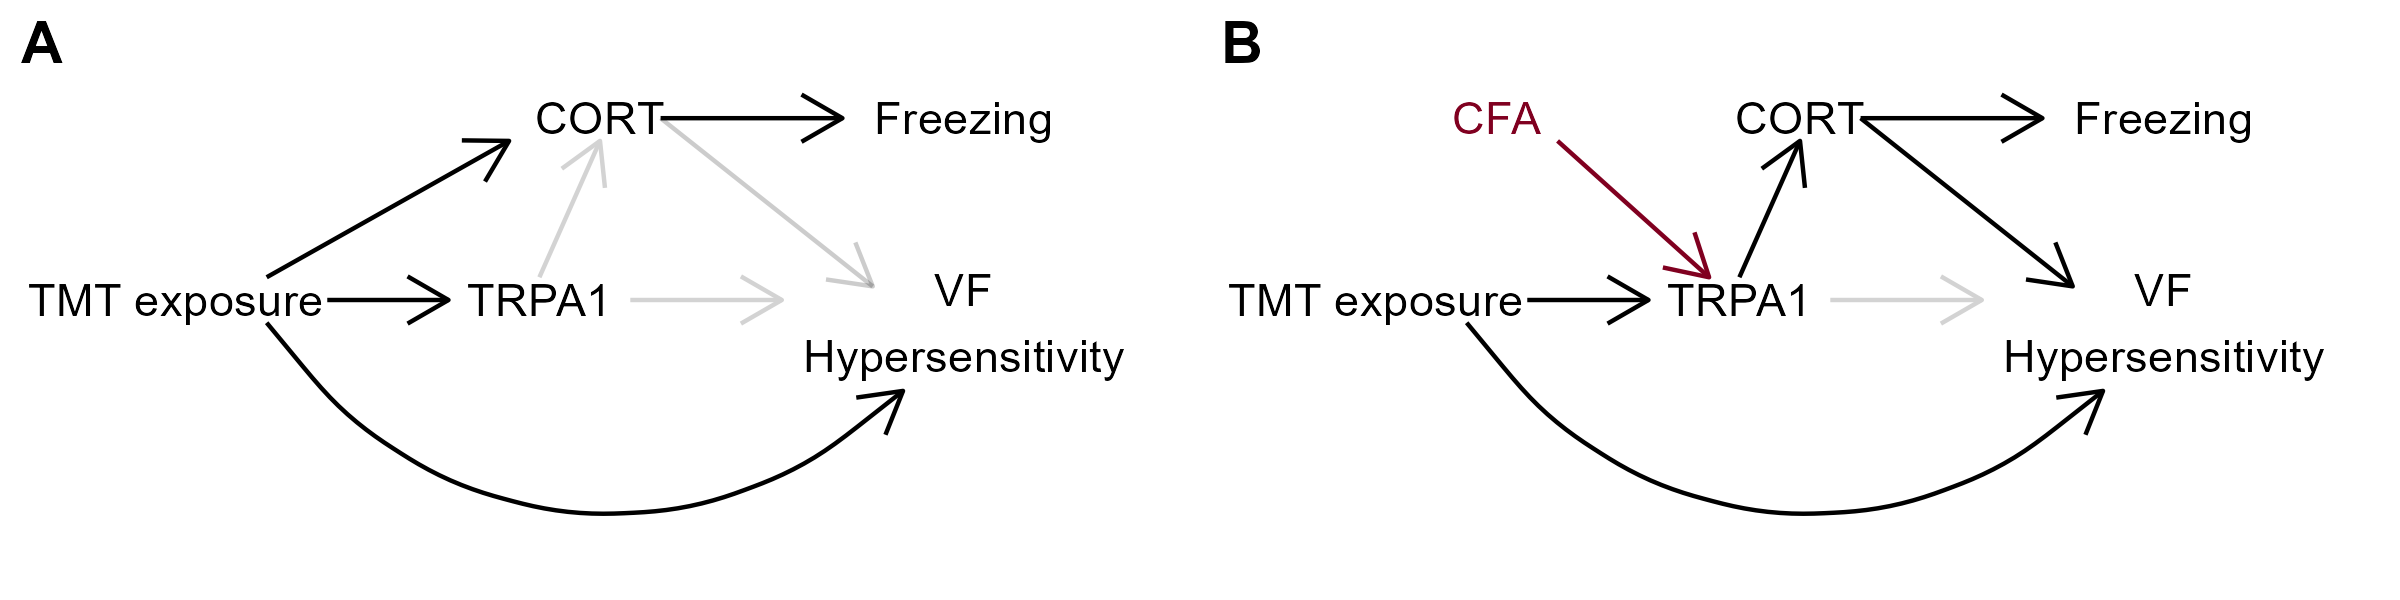
\includegraphics[width=33.33in]{Figs/7_Diagram}

\textbf{Figure 7. \emph{Proposed model of systems involved in behavioral responses to TMT.}} (A) Observed responses to TMT in pain-naive male mice. TMT induces two pharmacologically dissociable behavioral responses: Freezing behavior during the session and mechanical hypersensitivity after the exposure. The hormonal stress response entirely mediates freezing behavior, but corticosterone during TMT is not required for the expression of subsequent mechanical hypersensitivity. TRPA-1 signalling did not alter freezing behavior or mechanical sensitivity after TMT for naive mice, suggesting that, TMT induces mechanical hypersensitivity via corticosterone and TRPA-1-independent mechanisms (B) CFA-priming enhanced TMT-induced corticosterone levels, and this enhancement was blocked by pharmacological inhibition of TRPA-1 signalling. Together, these findings suggest that CFA-priming alters TRPA-1 signalling during TMT exposure to facilitate an enhanced corticosterone response, which causes enhanced freezing behavior during the session and a prolongation of mechanical sensitivity after the exposure.

The current results give rise to several novel insights about responses to TMT and modulation by prior experience with pain. Specifically, our findings indicate that TMT induces two pharmacologically dissociable behavioral responses: Freezing and mechanical hypersensitivity (Figure 7A). The hormonal stress response entirely mediates freezing, whereas hypersensitivity after TMT persists even when the stress response is blocked.

CFA-primed mice exhibit enhanced freezing and corticosterone release during TMT presentation, and prolonged sensitivity afterward. The freezing response can be entirely blocked by inhibition of glucocorticoid synthesis, and antagonism of TRPA-1 signaling normalized both freezing and circulating corticosterone among mice with a history of CFA injury (Figure 7B). These findings suggest that CFA-priming regulates TRAP-1 signaling to enhance threat-induced corticosterone release and the associated behavioral output - freezing. The enhanced hormonal stress response also modulated the prolongation of mechanical sensitivity after TMT without preventing TMT-induced hypersensitivity.

\chapter*{Supplemental Figure 1}\label{supplemental-figure-1}
\addcontentsline{toc}{chapter}{Supplemental Figure 1}

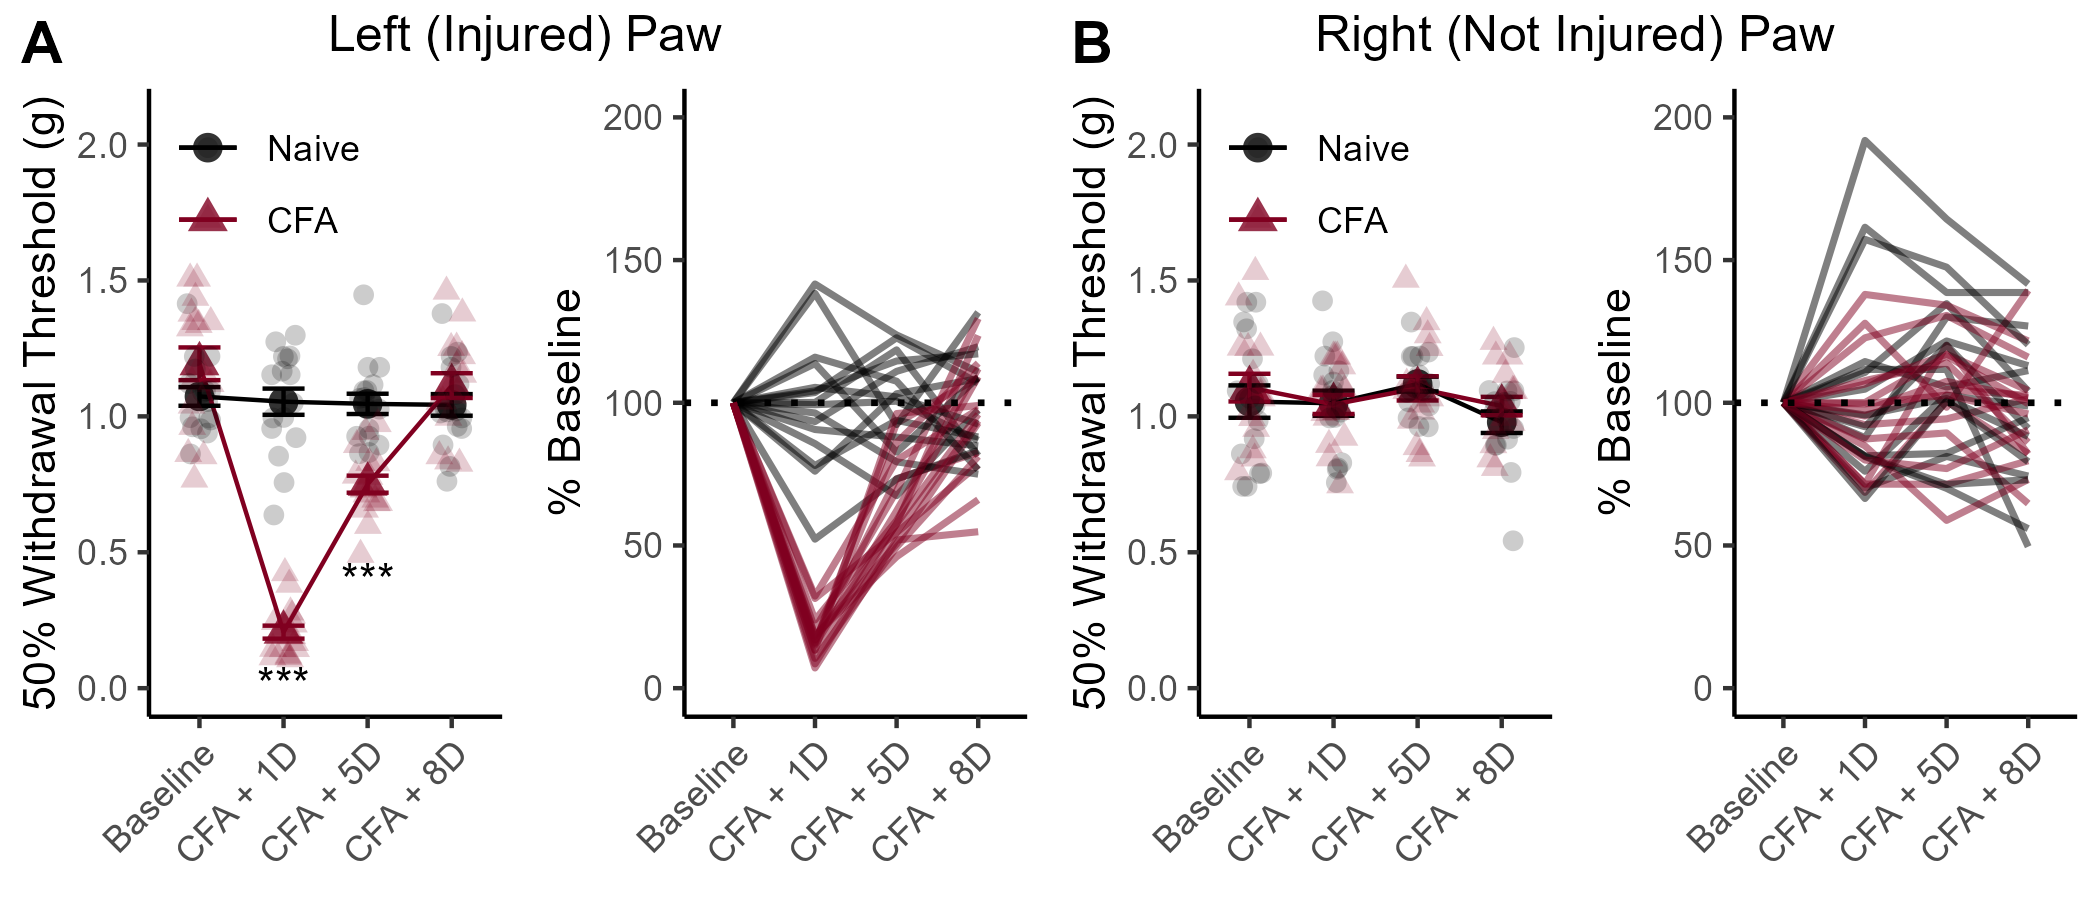
\includegraphics[width=29.17in]{Figs/S1_CFA_Recover}

\textbf{Supplemental Figure 1}. Time course of hypersensitivity and injury resolution after CFA administration. (A) CFA induces mechanical sensitivity at the site of injury. (B) CFA administration to the left paw did not produced changes in sensitivity in the contralateral paw. Data displayed as mean value +/- SEM.

\section*{Raw VF Values}\label{raw-vf-values}
\addcontentsline{toc}{section}{Raw VF Values}

\subsection*{Left Paws}\label{left-paws-1}
\addcontentsline{toc}{subsection}{Left Paws}

\begin{Shaded}
\begin{Highlighting}[]
\NormalTok{a }\OtherTok{\textless{}{-}}\NormalTok{ data[data}\SpecialCharTok{$}\NormalTok{Paw }\SpecialCharTok{==} \StringTok{"Left"}\NormalTok{, ]}
\FunctionTok{anova\_test}\NormalTok{(}\AttributeTok{data =}\NormalTok{ a, }\AttributeTok{dv=}\NormalTok{VF,}\AttributeTok{wid=}\NormalTok{ID,}\AttributeTok{between=}\NormalTok{CFA,}\AttributeTok{within=}\NormalTok{Test,}\AttributeTok{effect.size =} \StringTok{"pes"}\NormalTok{)}
\end{Highlighting}
\end{Shaded}

\begin{verbatim}
## ANOVA Table (type II tests)
## 
## $ANOVA
##     Effect DFn DFd      F        p p<.05   pes
## 1      CFA   1  30 45.385 1.82e-07     * 0.602
## 2     Test   3  90 70.641 1.42e-23     * 0.702
## 3 CFA:Test   3  90 68.662 3.46e-23     * 0.696
## 
## $`Mauchly's Test for Sphericity`
##     Effect     W     p p<.05
## 1     Test 0.913 0.761      
## 2 CFA:Test 0.913 0.761      
## 
## $`Sphericity Corrections`
##     Effect   GGe      DF[GG]    p[GG] p[GG]<.05   HFe      DF[HF]    p[HF]
## 1     Test 0.949 2.85, 85.37 1.76e-22         * 1.058 3.17, 95.25 1.42e-23
## 2 CFA:Test 0.949 2.85, 85.37 4.09e-22         * 1.058 3.17, 95.25 3.46e-23
##   p[HF]<.05
## 1         *
## 2         *
\end{verbatim}

\begin{Shaded}
\begin{Highlighting}[]
\NormalTok{a }\SpecialCharTok{\%\textgreater{}\%}
\NormalTok{  dplyr}\SpecialCharTok{::}\FunctionTok{group\_by}\NormalTok{(Test) }\SpecialCharTok{\%\textgreater{}\%}
  \FunctionTok{pairwise\_t\_test}\NormalTok{(VF}\SpecialCharTok{\textasciitilde{}}\NormalTok{CFA)}
\end{Highlighting}
\end{Shaded}

\begin{verbatim}
## # A tibble: 4 x 10
##   Test   .y.   group1 group2    n1    n2        p p.signif    p.adj p.adj.signif
## * <chr>  <chr> <chr>  <chr>  <int> <int>    <dbl> <chr>       <dbl> <chr>       
## 1 Basel~ VF    Naive  CFA       16    16 9.33e- 2 ns       9.33e- 2 ns          
## 2 CFA +~ VF    Naive  CFA       16    16 4.70e-16 ****     4.70e-16 ****        
## 3 CFA +~ VF    Naive  CFA       16    16 1.15e- 6 ****     1.15e- 6 ****        
## 4 CFA +~ VF    Naive  CFA       16    16 2.49e- 1 ns       2.49e- 1 ns
\end{verbatim}

CFA administration caused mechanical hypersensitivity in the week after injection F\st{3,90} = 68.88, p \textless0.001. CFA-treated mice had significantly lower paw withdrawal thresholds one and five days after injection (both p \textless{} 0.001), but the group difference in sensitivity had resolved by the eighth day after injection (p = 0.249).

\subsection*{Right Paws}\label{right-paws-1}
\addcontentsline{toc}{subsection}{Right Paws}

\begin{Shaded}
\begin{Highlighting}[]
\NormalTok{a }\OtherTok{\textless{}{-}}\NormalTok{ data[data}\SpecialCharTok{$}\NormalTok{Paw }\SpecialCharTok{==} \StringTok{"Right"}\NormalTok{, ]}
\FunctionTok{anova\_test}\NormalTok{(}\AttributeTok{data =}\NormalTok{ a, }\AttributeTok{dv=}\NormalTok{VF,}\AttributeTok{wid=}\NormalTok{ID,}\AttributeTok{between=}\NormalTok{CFA,}\AttributeTok{within=}\NormalTok{Test,}\AttributeTok{effect.size =} \StringTok{"pes"}\NormalTok{)}
\end{Highlighting}
\end{Shaded}

\begin{verbatim}
## ANOVA Table (type II tests)
## 
## $ANOVA
##     Effect DFn DFd     F     p p<.05   pes
## 1      CFA   1  30 0.470 0.498       0.015
## 2     Test   3  90 2.215 0.092       0.069
## 3 CFA:Test   3  90 0.416 0.742       0.014
## 
## $`Mauchly's Test for Sphericity`
##     Effect     W    p p<.05
## 1     Test 0.853 0.47      
## 2 CFA:Test 0.853 0.47      
## 
## $`Sphericity Corrections`
##     Effect   GGe     DF[GG] p[GG] p[GG]<.05   HFe      DF[HF] p[HF] p[HF]<.05
## 1     Test 0.896 2.69, 80.6 0.099           0.992 2.98, 89.28 0.092          
## 2 CFA:Test 0.896 2.69, 80.6 0.720           0.992 2.98, 89.28 0.740
\end{verbatim}

\begin{Shaded}
\begin{Highlighting}[]
\NormalTok{a }\SpecialCharTok{\%\textgreater{}\%}
\NormalTok{  dplyr}\SpecialCharTok{::}\FunctionTok{group\_by}\NormalTok{(Test) }\SpecialCharTok{\%\textgreater{}\%}
  \FunctionTok{pairwise\_t\_test}\NormalTok{(VF}\SpecialCharTok{\textasciitilde{}}\NormalTok{CFA)}
\end{Highlighting}
\end{Shaded}

\begin{verbatim}
## # A tibble: 4 x 10
##   Test     .y.   group1 group2    n1    n2     p p.signif p.adj p.adj.signif
## * <chr>    <chr> <chr>  <chr>  <int> <int> <dbl> <chr>    <dbl> <chr>       
## 1 Baseline VF    Naive  CFA       16    16 0.517 ns       0.517 ns          
## 2 CFA + 1D VF    Naive  CFA       16    16 0.94  ns       0.94  ns          
## 3 CFA + 5D VF    Naive  CFA       16    16 0.762 ns       0.762 ns          
## 4 CFA + 8D VF    Naive  CFA       16    16 0.262 ns       0.262 ns
\end{verbatim}

There was no effect of CFA treatment on VF thresholds for the right (non-injected) hindpaws across days of testing (p = 0.74)

\section*{Within-Subjects' Changes in VF Threasholds}\label{within-subjects-changes-in-vf-threasholds}
\addcontentsline{toc}{section}{Within-Subjects' Changes in VF Threasholds}

\begin{Shaded}
\begin{Highlighting}[]
\NormalTok{a }\OtherTok{\textless{}{-}}\NormalTok{ data }\SpecialCharTok{\%\textgreater{}\%}
  \FunctionTok{pivot\_wider}\NormalTok{(}\AttributeTok{names\_from =}\NormalTok{ Test, }\AttributeTok{values\_from =}\NormalTok{ VF) }\SpecialCharTok{\%\textgreater{}\%}
  \FunctionTok{mutate}\NormalTok{(}\AttributeTok{percBL\_1D =}\NormalTok{ (}\StringTok{\textasciigrave{}}\AttributeTok{CFA + 1D}\StringTok{\textasciigrave{}} \SpecialCharTok{/}\NormalTok{ Baseline) }\SpecialCharTok{*} \DecValTok{100}\NormalTok{,}
         \AttributeTok{percBL\_5D =}\NormalTok{ (}\StringTok{\textasciigrave{}}\AttributeTok{CFA + 5D}\StringTok{\textasciigrave{}} \SpecialCharTok{/}\NormalTok{ Baseline) }\SpecialCharTok{*} \DecValTok{100}\NormalTok{,}
         \AttributeTok{percBL\_8D =}\NormalTok{ (}\StringTok{\textasciigrave{}}\AttributeTok{CFA + 8D}\StringTok{\textasciigrave{}} \SpecialCharTok{/}\NormalTok{ Baseline) }\SpecialCharTok{*} \DecValTok{100}\NormalTok{,}
         \AttributeTok{Baseline =} \DecValTok{100}\NormalTok{) }\SpecialCharTok{\%\textgreater{}\%}
  \FunctionTok{select}\NormalTok{(ID, Paw, CFA, Baseline, percBL\_1D, percBL\_5D, percBL\_8D)}

\FunctionTok{colnames}\NormalTok{(a) }\OtherTok{\textless{}{-}} \FunctionTok{c}\NormalTok{(}\StringTok{"ID"}\NormalTok{,}\StringTok{"Paw"}\NormalTok{,}\StringTok{"CFA"}\NormalTok{,}\StringTok{"Baseline"}\NormalTok{,}\StringTok{"CFA + 1D"}\NormalTok{, }\StringTok{"CFA + 5D"}\NormalTok{, }\StringTok{"CFA + 8D"}\NormalTok{)}
\end{Highlighting}
\end{Shaded}

\subsection*{Left Paws}\label{left-paws-2}
\addcontentsline{toc}{subsection}{Left Paws}

\begin{Shaded}
\begin{Highlighting}[]
\NormalTok{b }\OtherTok{\textless{}{-}}\NormalTok{ a  }\SpecialCharTok{\%\textgreater{}\%}
  \FunctionTok{melt}\NormalTok{(}\AttributeTok{id.vars =} \FunctionTok{c}\NormalTok{(}\StringTok{"ID"}\NormalTok{, }\StringTok{"Paw"}\NormalTok{, }\StringTok{"CFA"}\NormalTok{)) }\SpecialCharTok{\%\textgreater{}\%}
  \FunctionTok{filter}\NormalTok{(Paw }\SpecialCharTok{==} \StringTok{"Left"}\NormalTok{) }\SpecialCharTok{\%\textgreater{}\%}
  \FunctionTok{ungroup}\NormalTok{() }

\FunctionTok{anova\_test}\NormalTok{(}\AttributeTok{data =}\NormalTok{ b, }\AttributeTok{dv =}\NormalTok{ value, }\AttributeTok{within =}\NormalTok{ variable, }\AttributeTok{between =}\NormalTok{ CFA, }\AttributeTok{wid =}\NormalTok{ ID)}
\end{Highlighting}
\end{Shaded}

\begin{verbatim}
## ANOVA Table (type II tests)
## 
## $ANOVA
##         Effect DFn DFd      F        p p<.05   ges
## 1          CFA   1  30 74.003 1.35e-09     * 0.507
## 2     variable   3  90 65.910 1.23e-22     * 0.561
## 3 CFA:variable   3  90 67.574 5.69e-23     * 0.568
## 
## $`Mauchly's Test for Sphericity`
##         Effect     W    p p<.05
## 1     variable 0.911 0.75      
## 2 CFA:variable 0.911 0.75      
## 
## $`Sphericity Corrections`
##         Effect   GGe     DF[GG]    p[GG] p[GG]<.05   HFe      DF[HF]    p[HF]
## 1     variable 0.946 2.84, 85.1 1.57e-21         * 1.055 3.16, 94.91 1.23e-22
## 2 CFA:variable 0.946 2.84, 85.1 7.55e-22         * 1.055 3.16, 94.91 5.69e-23
##   p[HF]<.05
## 1         *
## 2         *
\end{verbatim}

\begin{Shaded}
\begin{Highlighting}[]
\NormalTok{b }\SpecialCharTok{\%\textgreater{}\%}
  \FunctionTok{group\_by}\NormalTok{(CFA) }\SpecialCharTok{\%\textgreater{}\%}
  \FunctionTok{pairwise\_t\_test}\NormalTok{(value}\SpecialCharTok{\textasciitilde{}}\NormalTok{variable, }\AttributeTok{paired =}\NormalTok{ T)}
\end{Highlighting}
\end{Shaded}

\begin{verbatim}
## # A tibble: 12 x 11
##    CFA   .y.   group1   group2      n1    n2 statistic    df        p    p.adj
##  * <fct> <chr> <chr>    <chr>    <int> <int>     <dbl> <dbl>    <dbl>    <dbl>
##  1 Naive value Baseline CFA + 1D    16    16    0.0603    15 9.53e- 1 1   e+ 0
##  2 Naive value Baseline CFA + 5D    16    16    0.273     15 7.88e- 1 1   e+ 0
##  3 Naive value Baseline CFA + 8D    16    16    0.445     15 6.63e- 1 1   e+ 0
##  4 Naive value CFA + 1D CFA + 5D    16    16    0.162     15 8.73e- 1 1   e+ 0
##  5 Naive value CFA + 1D CFA + 8D    16    16    0.293     15 7.74e- 1 1   e+ 0
##  6 Naive value CFA + 5D CFA + 8D    16    16    0.136     15 8.93e- 1 1   e+ 0
##  7 CFA   value Baseline CFA + 1D    16    16   46.7       15 1.18e-17 7.08e-17
##  8 CFA   value Baseline CFA + 5D    16    16    8.72      15 2.93e- 7 8.79e- 7
##  9 CFA   value Baseline CFA + 8D    16    16    0.752     15 4.64e- 1 4.64e- 1
## 10 CFA   value CFA + 1D CFA + 5D    16    16  -11.3       15 9.5 e- 9 3.8 e- 8
## 11 CFA   value CFA + 1D CFA + 8D    16    16  -15.6       15 1.09e-10 5.45e-10
## 12 CFA   value CFA + 5D CFA + 8D    16    16   -6.38      15 1.24e- 5 2.48e- 5
## # i 1 more variable: p.adj.signif <chr>
\end{verbatim}

CFA induced significant changes in VF thresholds across the time course F\st{3,90} = 67.57, p \textless{} 0.001. CFA-treated mice exhibited significant decreases in their paw withdrawal thresholds, relative to their baseline measurements, both one and five days after injection (both p \textless{} 0.001). CFA-treated mice did not exhibit ongoing sensitivity eight days after CFA injection, indicating that the injury had resolved (p = 0.464).

\subsection*{Right Paws}\label{right-paws-2}
\addcontentsline{toc}{subsection}{Right Paws}

\begin{Shaded}
\begin{Highlighting}[]
\NormalTok{b }\OtherTok{\textless{}{-}}\NormalTok{ a }\SpecialCharTok{\%\textgreater{}\%}
  \FunctionTok{melt}\NormalTok{(}\AttributeTok{id.vars =} \FunctionTok{c}\NormalTok{(}\StringTok{"ID"}\NormalTok{, }\StringTok{"Paw"}\NormalTok{, }\StringTok{"CFA"}\NormalTok{)) }\SpecialCharTok{\%\textgreater{}\%}
  \FunctionTok{filter}\NormalTok{(Paw }\SpecialCharTok{==} \StringTok{"Right"}\NormalTok{) }\SpecialCharTok{\%\textgreater{}\%}
  \FunctionTok{ungroup}\NormalTok{()}

\FunctionTok{anova\_test}\NormalTok{(}\AttributeTok{data =}\NormalTok{ b, }\AttributeTok{dv =}\NormalTok{ value, }\AttributeTok{within =}\NormalTok{ variable, }\AttributeTok{between =}\NormalTok{ CFA, }\AttributeTok{wid =}\NormalTok{ ID)}
\end{Highlighting}
\end{Shaded}

\begin{verbatim}
## ANOVA Table (type II tests)
## 
## $ANOVA
##         Effect DFn DFd     F     p p<.05   ges
## 1          CFA   1  30 0.580 0.452       0.012
## 2     variable   3  90 2.110 0.105       0.027
## 3 CFA:variable   3  90 0.676 0.569       0.009
## 
## $`Mauchly's Test for Sphericity`
##         Effect     W    p p<.05
## 1     variable 0.738 0.12      
## 2 CFA:variable 0.738 0.12      
## 
## $`Sphericity Corrections`
##         Effect   GGe      DF[GG] p[GG] p[GG]<.05   HFe      DF[HF] p[HF]
## 1     variable 0.816 2.45, 73.47 0.118           0.894 2.68, 80.49 0.112
## 2 CFA:variable 0.816 2.45, 73.47 0.540           0.894 2.68, 80.49 0.553
##   p[HF]<.05
## 1          
## 2
\end{verbatim}

There were no within-subjects changes in paw withdrawal thresholds for the right (non-injured) paws (p = 0.57).

\chapter*{Supplemental Figure 2}\label{supplemental-figure-2}
\addcontentsline{toc}{chapter}{Supplemental Figure 2}

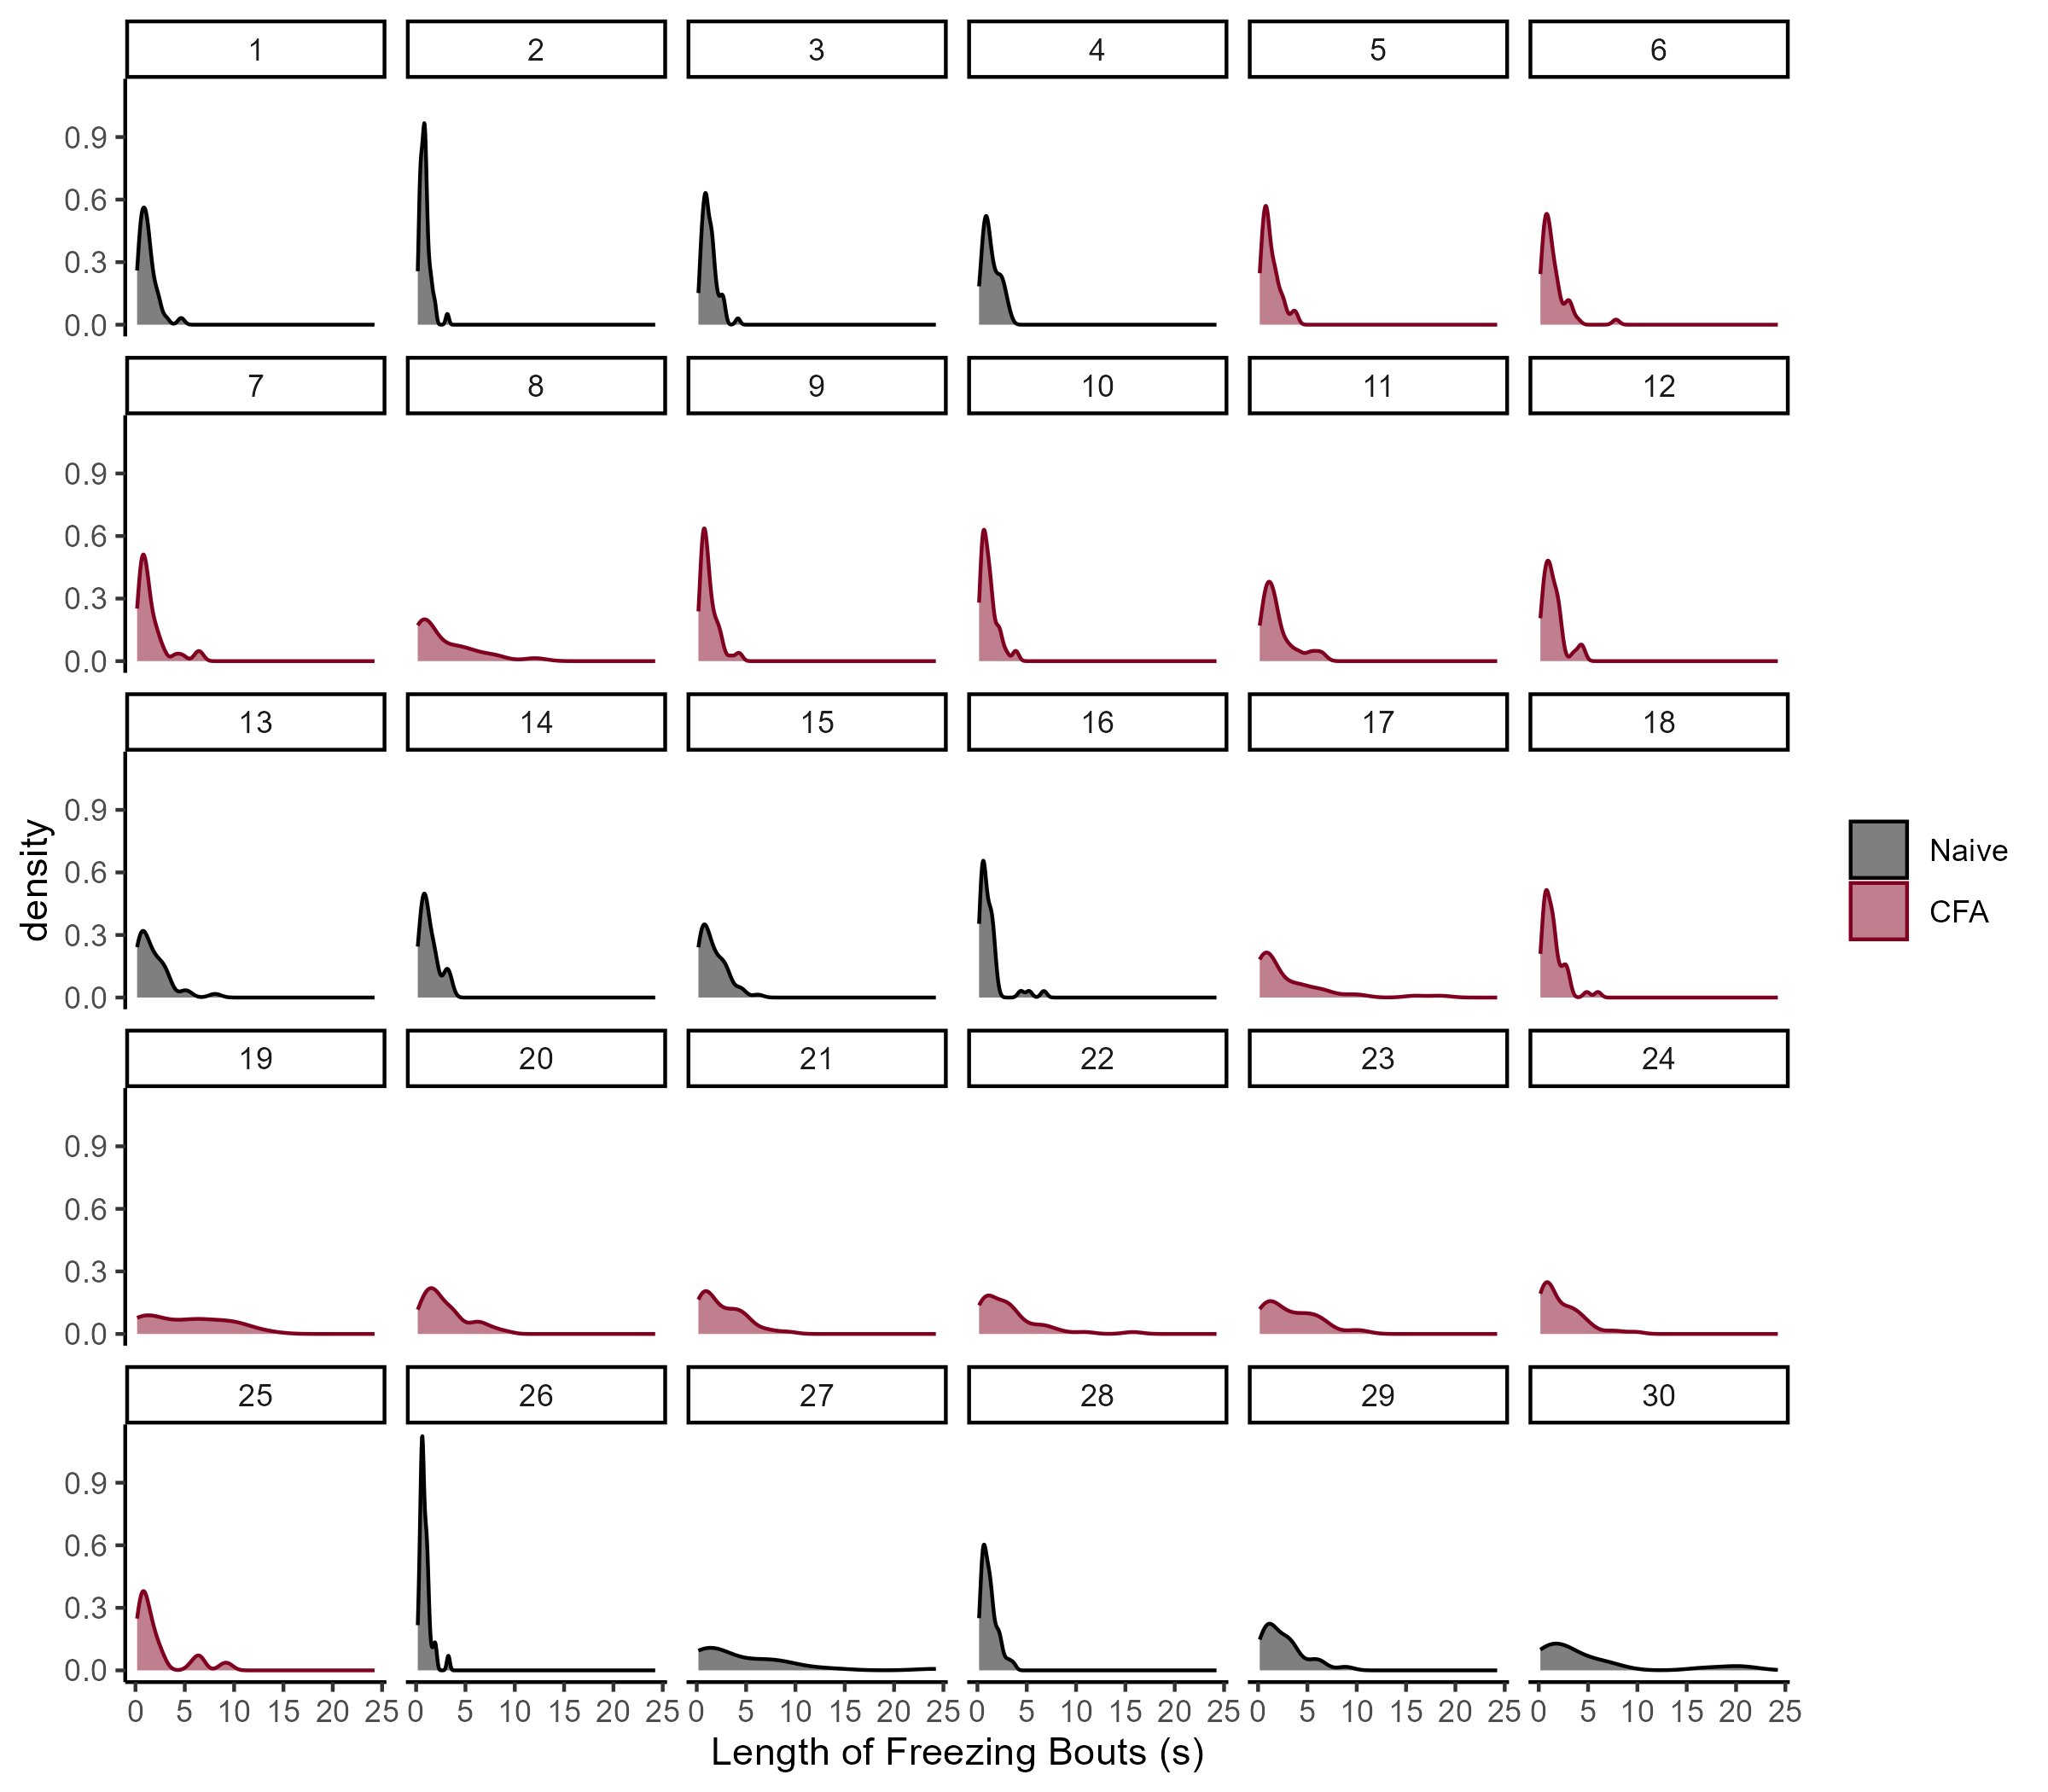
\includegraphics[width=33.33in]{Figs/S2_Individuals_Frz}

\textbf{Supplemental Figure 2}. Distributions of the lengths of bouts of freezing during TMT for the 30 mice shown in Figure 1 of the main text. For every individual, the distributions of freezing episodes are right-skewed, indicating that mice exhibit many shorter bouts of freezing along with fewer longer episodes.

\begin{Shaded}
\begin{Highlighting}[]
\FunctionTok{library}\NormalTok{(moments)}
\NormalTok{skew\_df }\OtherTok{\textless{}{-}}\NormalTok{ a }\SpecialCharTok{\%\textgreater{}\%}
  \FunctionTok{group\_by}\NormalTok{(ID) }\SpecialCharTok{\%\textgreater{}\%}
  \FunctionTok{summarise}\NormalTok{(}
    \AttributeTok{skew =} \FunctionTok{skewness}\NormalTok{(Duration)}
\NormalTok{  )}

\FunctionTok{t.test}\NormalTok{(skew\_df}\SpecialCharTok{$}\NormalTok{skew, }\AttributeTok{mu =} \DecValTok{0}\NormalTok{, }\AttributeTok{alternative =} \StringTok{"greater"}\NormalTok{)}
\end{Highlighting}
\end{Shaded}

\begin{verbatim}
## 
##  One Sample t-test
## 
## data:  skew_df$skew
## t = 14.66, df = 29, p-value = 3.031e-15
## alternative hypothesis: true mean is greater than 0
## 95 percent confidence interval:
##  1.379179      Inf
## sample estimates:
## mean of x 
##  1.559989
\end{verbatim}

The distributions of bout durations of freezing responses are heavily right-skewed during TMT presentation (t\textsubscript{29} = 14.66, p \textless{} 0.001). For this reason, aggregating the behavior by calculating the mean length of freeze for each mouse would not be statistically appropriate. Instead, we aggregated all the freezing episodes for each condition, and compared the resultant distributions between groups in our analyses.

\chapter*{Supplemental Figure 3}\label{supplemental-figure-3}
\addcontentsline{toc}{chapter}{Supplemental Figure 3}

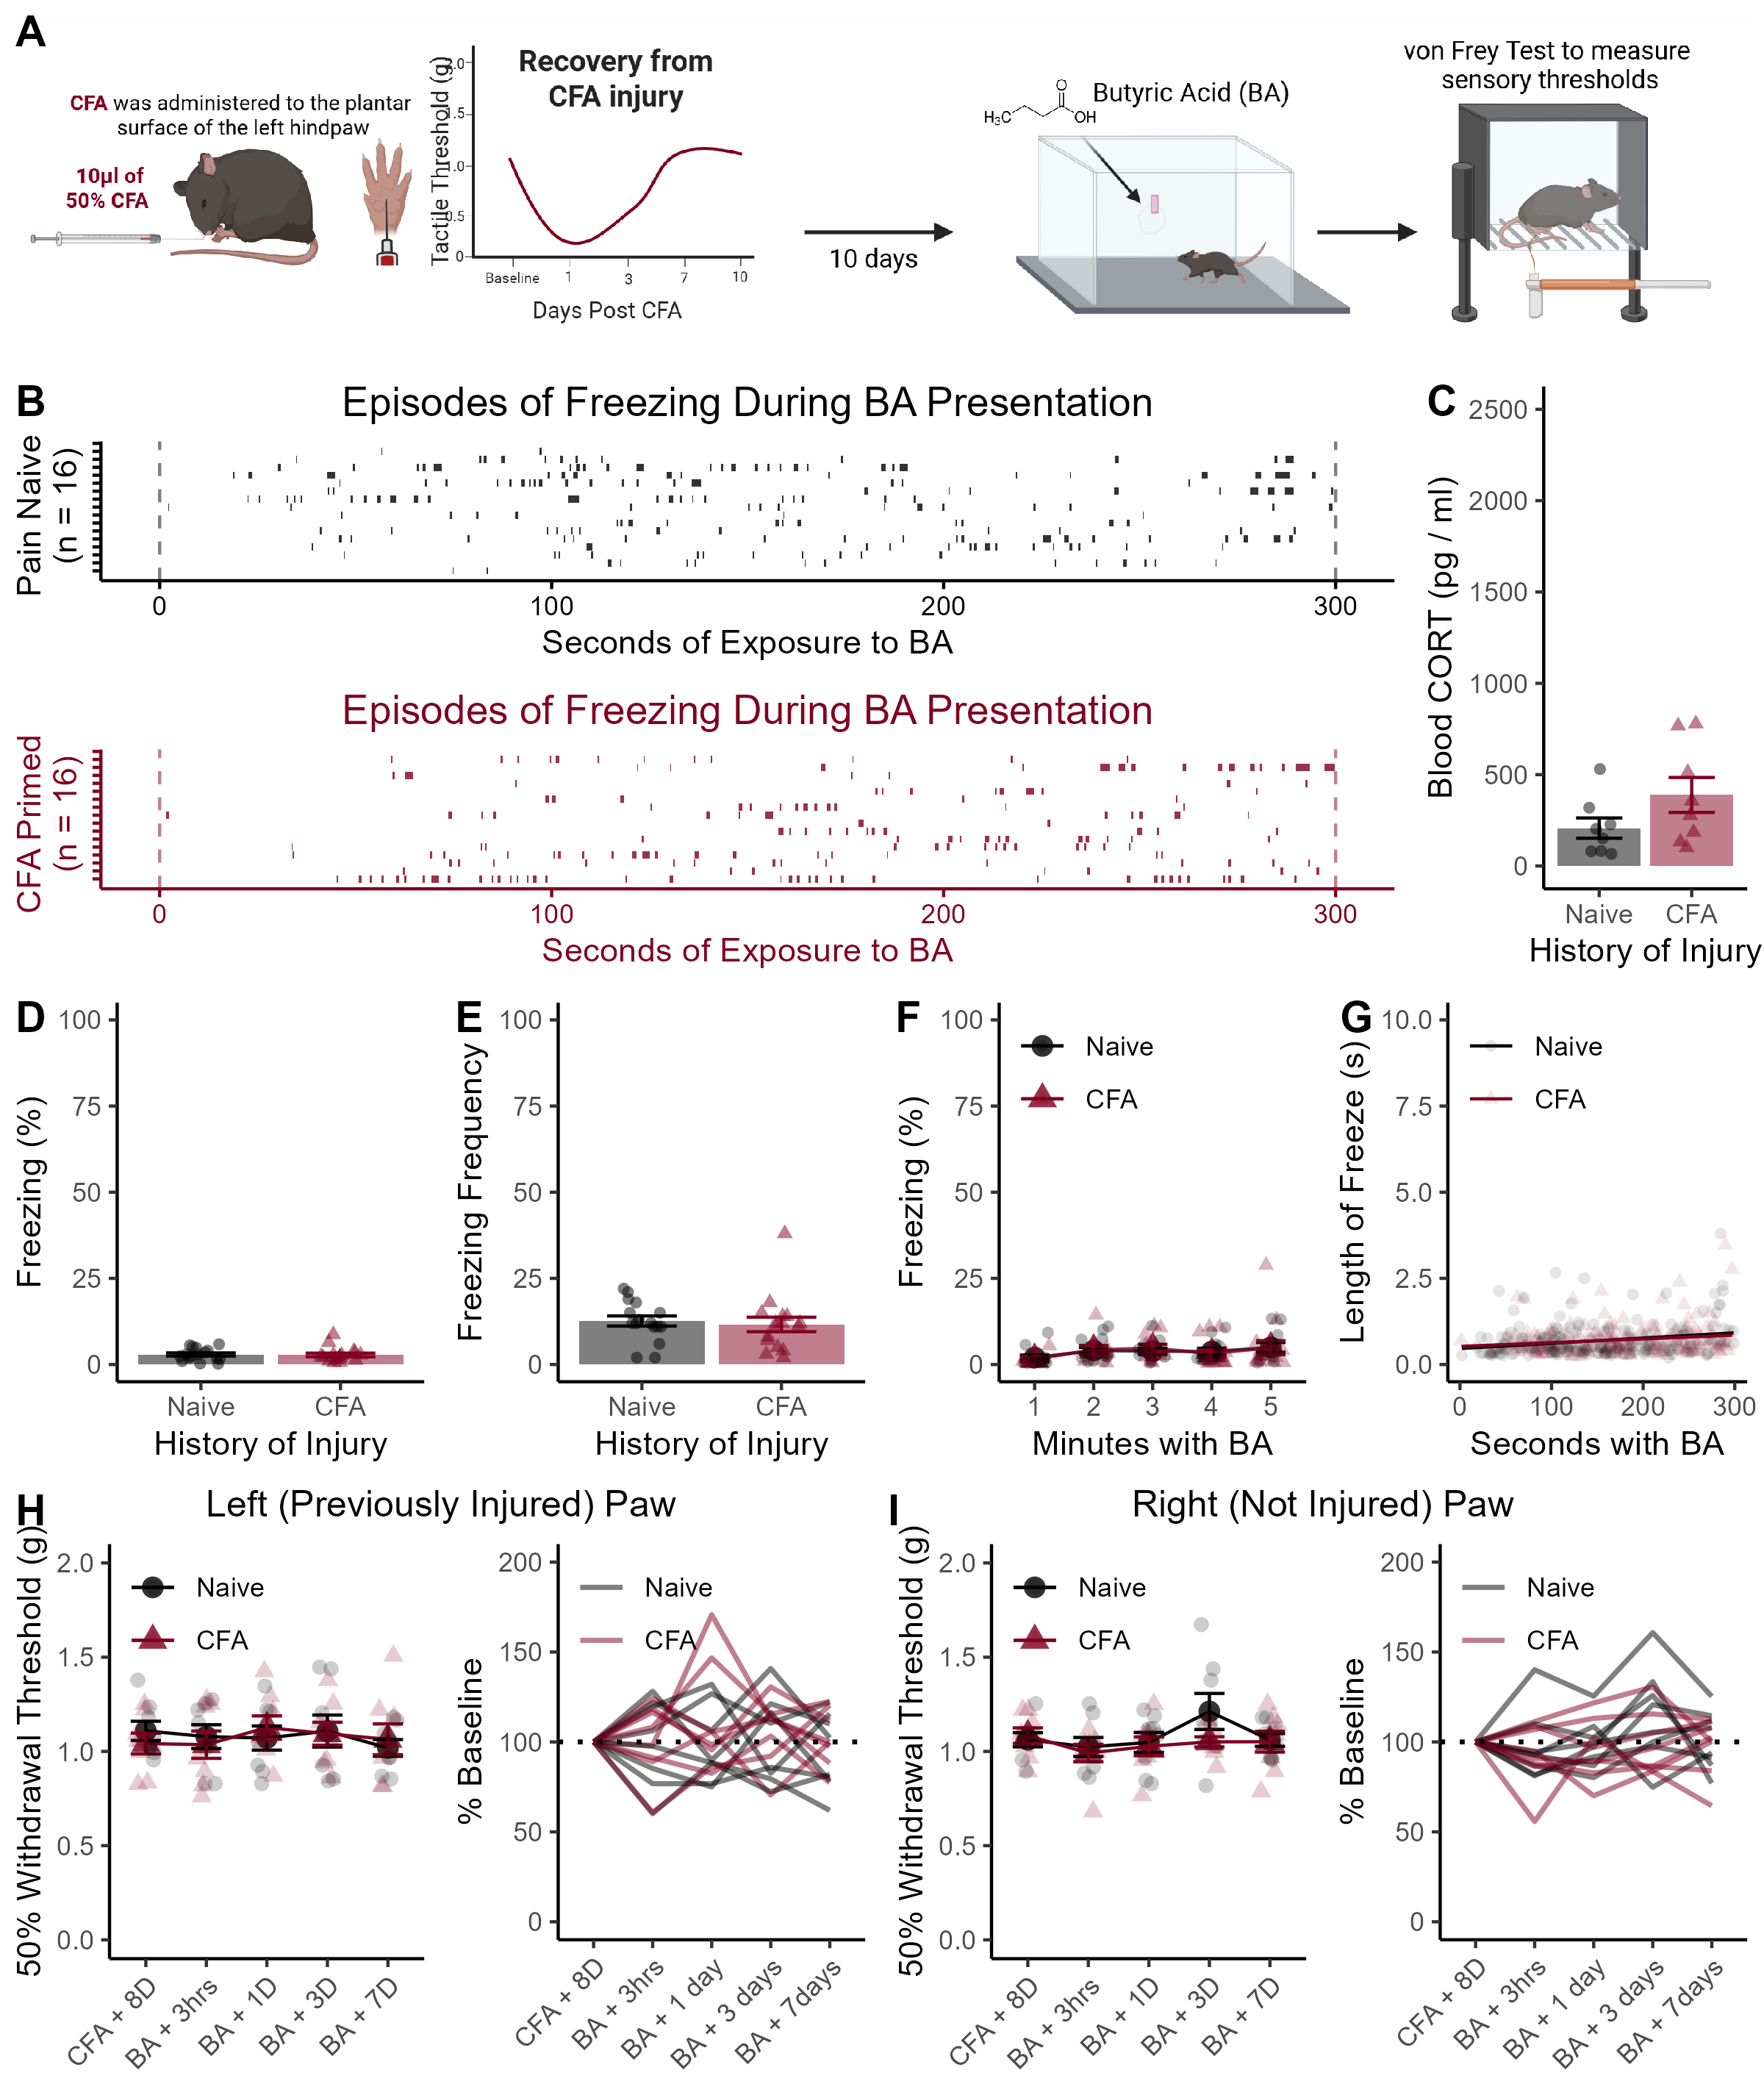
\includegraphics[width=33.33in]{Figs/S3_BA_Panel}

\textbf{Supplemental Figure 3}. Behavioral, hormonal, and sensory responses to butyric acid presentation. (A) Timeline of experimental proceedings. Mice were placed in an apparatus with 35 \(\mu l\) of 10\% butyric acid 10 days after CFA administration. (B) Raster plots of individual freezing episodes during the butyric acid session. (C) Circulating levels of CORT 30 minutes after butyric acid presentation. (D) Average freezing during butryic acid was very low. (E) Number of freezing episodes during the five-minute exposure to butyric acid. (F) The amount of time spent freezing did not increase across the five minutes of the test. (G) There was no significant increase in length of freezing episodes across the five minute session. (H) There was no change in mechanical thresholds at the site of previous CFA injury after the butyric acid exposure, or (I) the opposite (not previously injured) hind paw. Data presented as mean value +/- SEM

\section*{CORT Levels}\label{cort-levels}
\addcontentsline{toc}{section}{CORT Levels}

\begin{Shaded}
\begin{Highlighting}[]
\FunctionTok{t.test}\NormalTok{(}\AttributeTok{data =}\NormalTok{ Cort\_data, CORT }\SpecialCharTok{\textasciitilde{}}\NormalTok{ CFA, }\AttributeTok{var.equal =}\NormalTok{ T)}
\end{Highlighting}
\end{Shaded}

\begin{verbatim}
## 
##  Two Sample t-test
## 
## data:  CORT by CFA
## t = -1.6381, df = 14, p-value = 0.1237
## alternative hypothesis: true difference in means between group Naive and group CFA is not equal to 0
## 95 percent confidence interval:
##  -418.7721   56.0936
## sample estimates:
## mean in group Naive   mean in group CFA 
##            207.3606            388.6998
\end{verbatim}

A history of CFA injury did not increase circulating CORT 30 minutes after the butyric acid session (p = 0.12, Figure S3C).

\section*{Time Spent Freezing During TMT}\label{time-spent-freezing-during-tmt-1}
\addcontentsline{toc}{section}{Time Spent Freezing During TMT}

\begin{Shaded}
\begin{Highlighting}[]
\NormalTok{b }\OtherTok{\textless{}{-}}\NormalTok{ Exp\_1\_CFA.N  }\SpecialCharTok{\%\textgreater{}\%}
  \FunctionTok{filter}\NormalTok{(Behavior }\SpecialCharTok{==} \StringTok{"freeze"}\NormalTok{) }\SpecialCharTok{\%\textgreater{}\%}
  \FunctionTok{group\_by}\NormalTok{(ID,CFA) }\SpecialCharTok{\%\textgreater{}\%}
  \FunctionTok{summarise}\NormalTok{(}
    \AttributeTok{sum=}\FunctionTok{sum}\NormalTok{(Duration),}
    \AttributeTok{Number=}\FunctionTok{n}\NormalTok{(),}
\NormalTok{  ) }\SpecialCharTok{\%\textgreater{}\%}
  \FunctionTok{mutate}\NormalTok{(}\AttributeTok{Perc =}\NormalTok{ (sum }\SpecialCharTok{/} \DecValTok{300}\NormalTok{)}\SpecialCharTok{*}\DecValTok{100}\NormalTok{) }
\end{Highlighting}
\end{Shaded}

\begin{verbatim}
## `summarise()` has grouped output by 'ID'. You can override using the `.groups`
## argument.
\end{verbatim}

\begin{Shaded}
\begin{Highlighting}[]
\FunctionTok{t.test}\NormalTok{(Perc}\SpecialCharTok{\textasciitilde{}}\NormalTok{CFA,}\AttributeTok{data=}\NormalTok{b,}\AttributeTok{var.equal=}\ConstantTok{TRUE}\NormalTok{)}
\end{Highlighting}
\end{Shaded}

\begin{verbatim}
## 
##  Two Sample t-test
## 
## data:  Perc by CFA
## t = 0.2122, df = 30, p-value = 0.8334
## alternative hypothesis: true difference in means between group Naive and group CFA is not equal to 0
## 95 percent confidence interval:
##  -1.275518  1.571310
## sample estimates:
## mean in group Naive   mean in group CFA 
##            2.918896            2.771000
\end{verbatim}

There was no group difference in the amount of time spent freezing (p = 0.83, Figure S3D).

\section*{Freezing Frequency During TMT}\label{freezing-frequency-during-tmt-1}
\addcontentsline{toc}{section}{Freezing Frequency During TMT}

\begin{Shaded}
\begin{Highlighting}[]
\NormalTok{b }\OtherTok{\textless{}{-}}\NormalTok{ Exp\_1\_CFA.N  }\SpecialCharTok{\%\textgreater{}\%}
  \FunctionTok{filter}\NormalTok{(Behavior }\SpecialCharTok{==} \StringTok{"freeze"}\NormalTok{) }\SpecialCharTok{\%\textgreater{}\%}
  \FunctionTok{group\_by}\NormalTok{(ID,CFA) }\SpecialCharTok{\%\textgreater{}\%}
  \FunctionTok{summarise}\NormalTok{(}
    \AttributeTok{sum=}\FunctionTok{sum}\NormalTok{(Duration),}
    \AttributeTok{Number=}\FunctionTok{n}\NormalTok{(),}
\NormalTok{  )}
\end{Highlighting}
\end{Shaded}

\begin{verbatim}
## `summarise()` has grouped output by 'ID'. You can override using the `.groups`
## argument.
\end{verbatim}

\begin{Shaded}
\begin{Highlighting}[]
\FunctionTok{t.test}\NormalTok{(Number}\SpecialCharTok{\textasciitilde{}}\NormalTok{CFA,}\AttributeTok{data=}\NormalTok{b,}\AttributeTok{var.equal=}\ConstantTok{TRUE}\NormalTok{)}
\end{Highlighting}
\end{Shaded}

\begin{verbatim}
## 
##  Two Sample t-test
## 
## data:  Number by CFA
## t = 0.38956, df = 30, p-value = 0.6996
## alternative hypothesis: true difference in means between group Naive and group CFA is not equal to 0
## 95 percent confidence interval:
##  -4.242551  6.242551
## sample estimates:
## mean in group Naive   mean in group CFA 
##              12.625              11.625
\end{verbatim}

There was no difference in frequency of freezing (p = 0.70, Figure S3E)

\section*{Freezing Each Minute With TMT}\label{freezing-each-minute-with-tmt}
\addcontentsline{toc}{section}{Freezing Each Minute With TMT}

\begin{Shaded}
\begin{Highlighting}[]
\NormalTok{a }\OtherTok{\textless{}{-}}\NormalTok{ Exp\_1\_CFA.N }\SpecialCharTok{\%\textgreater{}\%}
  \FunctionTok{na.omit}\NormalTok{() }\SpecialCharTok{\%\textgreater{}\%}
  \FunctionTok{mutate}\NormalTok{(}\AttributeTok{Bins =} \FunctionTok{cut}\NormalTok{(}
\NormalTok{    Start\_clean,}
    \AttributeTok{breaks =} \DecValTok{5}\NormalTok{,}
    \AttributeTok{labels=}\FunctionTok{c}\NormalTok{(}\StringTok{"1"}\NormalTok{,}\StringTok{"2"}\NormalTok{,}\StringTok{"3"}\NormalTok{,}\StringTok{"4"}\NormalTok{,}\StringTok{"5"}\NormalTok{)}
\NormalTok{  )) }\SpecialCharTok{\%\textgreater{}\%}
  \FunctionTok{group\_by}\NormalTok{(ID, Behavior, CFA, Bins) }\SpecialCharTok{\%\textgreater{}\%}
  \FunctionTok{summarise}\NormalTok{(}
    \AttributeTok{sum =} \FunctionTok{sum}\NormalTok{ (Duration)}
\NormalTok{  ) }\SpecialCharTok{\%\textgreater{}\%}
  \FunctionTok{mutate}\NormalTok{(}\AttributeTok{Perc =}\NormalTok{ (sum }\SpecialCharTok{/} \DecValTok{60}\NormalTok{)}\SpecialCharTok{*}\DecValTok{100}\NormalTok{ ) }\SpecialCharTok{\%\textgreater{}\%}
  \FunctionTok{filter}\NormalTok{(Behavior }\SpecialCharTok{==} \StringTok{"freeze"}\NormalTok{)}
\end{Highlighting}
\end{Shaded}

\begin{verbatim}
## `summarise()` has grouped output by 'ID', 'Behavior', 'CFA'. You can override
## using the `.groups` argument.
\end{verbatim}

\begin{Shaded}
\begin{Highlighting}[]
\NormalTok{res }\OtherTok{\textless{}{-}} \FunctionTok{aov}\NormalTok{(}\AttributeTok{data =}\NormalTok{ a, Perc }\SpecialCharTok{\textasciitilde{}}\NormalTok{ Bins)}
\FunctionTok{summary}\NormalTok{(res)}
\end{Highlighting}
\end{Shaded}

\begin{verbatim}
##              Df Sum Sq Mean Sq F value Pr(>F)
## Bins          4  115.7   28.93   1.672  0.161
## Residuals   114 1972.7   17.30
\end{verbatim}

Unlike the behavioral patterns observed during TMT presentation, there was no increase in the time spent freezing (p = 0.16, Figure S3F)

\section*{Linear Relationship Between Time and Length of Freeze}\label{linear-relationship-between-time-and-length-of-freeze-1}
\addcontentsline{toc}{section}{Linear Relationship Between Time and Length of Freeze}

\begin{Shaded}
\begin{Highlighting}[]
\NormalTok{b }\OtherTok{\textless{}{-}} \FunctionTok{lm}\NormalTok{(Duration}\SpecialCharTok{\textasciitilde{}}\NormalTok{Start\_clean }\SpecialCharTok{*}\NormalTok{ CFA, }\AttributeTok{data=}\NormalTok{Exp\_1\_CFA.N)}
\FunctionTok{summary}\NormalTok{(b)}
\end{Highlighting}
\end{Shaded}

\begin{verbatim}
## 
## Call:
## lm(formula = Duration ~ Start_clean * CFA, data = Exp_1_CFA.N)
## 
## Residuals:
##    Min     1Q Median     3Q    Max 
## -1.633 -1.151 -0.820 -0.102 33.441 
## 
## Coefficients:
##                     Estimate Std. Error t value Pr(>|t|)    
## (Intercept)        1.5093969  0.2665738   5.662 1.93e-08 ***
## Start_clean        0.0007741  0.0015560   0.497    0.619    
## CFACFA             0.1373560  0.3907523   0.352    0.725    
## Start_clean:CFACFA 0.0002573  0.0022362   0.115    0.908    
## ---
## Signif. codes:  0 '***' 0.001 '**' 0.01 '*' 0.05 '.' 0.1 ' ' 1
## 
## Residual standard error: 3.022 on 1055 degrees of freedom
##   (64 observations deleted due to missingness)
## Multiple R-squared:  0.00156,    Adjusted R-squared:  -0.001279 
## F-statistic: 0.5496 on 3 and 1055 DF,  p-value: 0.6485
\end{verbatim}

There was no increase in the length of freezing episodes (p = 0.50, Figure S3G) across the session.

\section*{Von Frey Paw Sensitivity}\label{von-frey-paw-sensitivity}
\addcontentsline{toc}{section}{Von Frey Paw Sensitivity}

\begin{Shaded}
\begin{Highlighting}[]
\NormalTok{data }\SpecialCharTok{\%\textgreater{}\%}
  \FunctionTok{filter}\NormalTok{(Paw }\SpecialCharTok{==} \StringTok{"Left"}\NormalTok{) }\SpecialCharTok{\%\textgreater{}\%}
  \FunctionTok{anova\_test}\NormalTok{(}\AttributeTok{dv =}\NormalTok{  VF, }\AttributeTok{within =}\NormalTok{ Test, }\AttributeTok{between =}\NormalTok{ CFA, }\AttributeTok{wid =}\NormalTok{ ID)}
\end{Highlighting}
\end{Shaded}

\begin{verbatim}
## ANOVA Table (type II tests)
## 
## $ANOVA
##     Effect DFn DFd     F     p p<.05      ges
## 1      CFA   1  14 0.012 0.916       0.000176
## 2     Test   4  56 0.324 0.861       0.018000
## 3 CFA:Test   4  56 0.350 0.843       0.019000
## 
## $`Mauchly's Test for Sphericity`
##     Effect     W    p p<.05
## 1     Test 0.665 0.83      
## 2 CFA:Test 0.665 0.83      
## 
## $`Sphericity Corrections`
##     Effect   GGe     DF[GG] p[GG] p[GG]<.05   HFe      DF[HF] p[HF] p[HF]<.05
## 1     Test 0.824 3.3, 46.16 0.826           1.109 4.43, 62.08 0.861          
## 2 CFA:Test 0.824 3.3, 46.16 0.808           1.109 4.43, 62.08 0.843
\end{verbatim}

\begin{Shaded}
\begin{Highlighting}[]
\NormalTok{data }\SpecialCharTok{\%\textgreater{}\%}
  \FunctionTok{filter}\NormalTok{(Paw }\SpecialCharTok{==} \StringTok{"Right"}\NormalTok{) }\SpecialCharTok{\%\textgreater{}\%}
  \FunctionTok{anova\_test}\NormalTok{(}\AttributeTok{dv =}\NormalTok{  VF, }\AttributeTok{within =}\NormalTok{ Test, }\AttributeTok{between =}\NormalTok{ CFA, }\AttributeTok{wid =}\NormalTok{ ID)}
\end{Highlighting}
\end{Shaded}

\begin{verbatim}
## ANOVA Table (type II tests)
## 
## $ANOVA
##     Effect DFn DFd     F     p p<.05   ges
## 1      CFA   1  14 1.136 0.304       0.021
## 2     Test   4  56 1.708 0.161       0.082
## 3 CFA:Test   4  56 0.995 0.418       0.050
## 
## $`Mauchly's Test for Sphericity`
##     Effect     W     p p<.05
## 1     Test 0.368 0.194      
## 2 CFA:Test 0.368 0.194      
## 
## $`Sphericity Corrections`
##     Effect   GGe      DF[GG] p[GG] p[GG]<.05   HFe      DF[HF] p[HF] p[HF]<.05
## 1     Test 0.731 2.92, 40.91 0.182           0.944 3.78, 52.87 0.165          
## 2 CFA:Test 0.731 2.92, 40.91 0.403           0.944 3.78, 52.87 0.415
\end{verbatim}

There were no changes in mechanical thresholds after butyric acid (Left paw: all p \textgreater{} 0.84; Right paw: all p \textgreater{} .16, Figure S3H \& I, respectively).

\chapter*{Supplemental Figure 4}\label{supplemental-figure-4}
\addcontentsline{toc}{chapter}{Supplemental Figure 4}

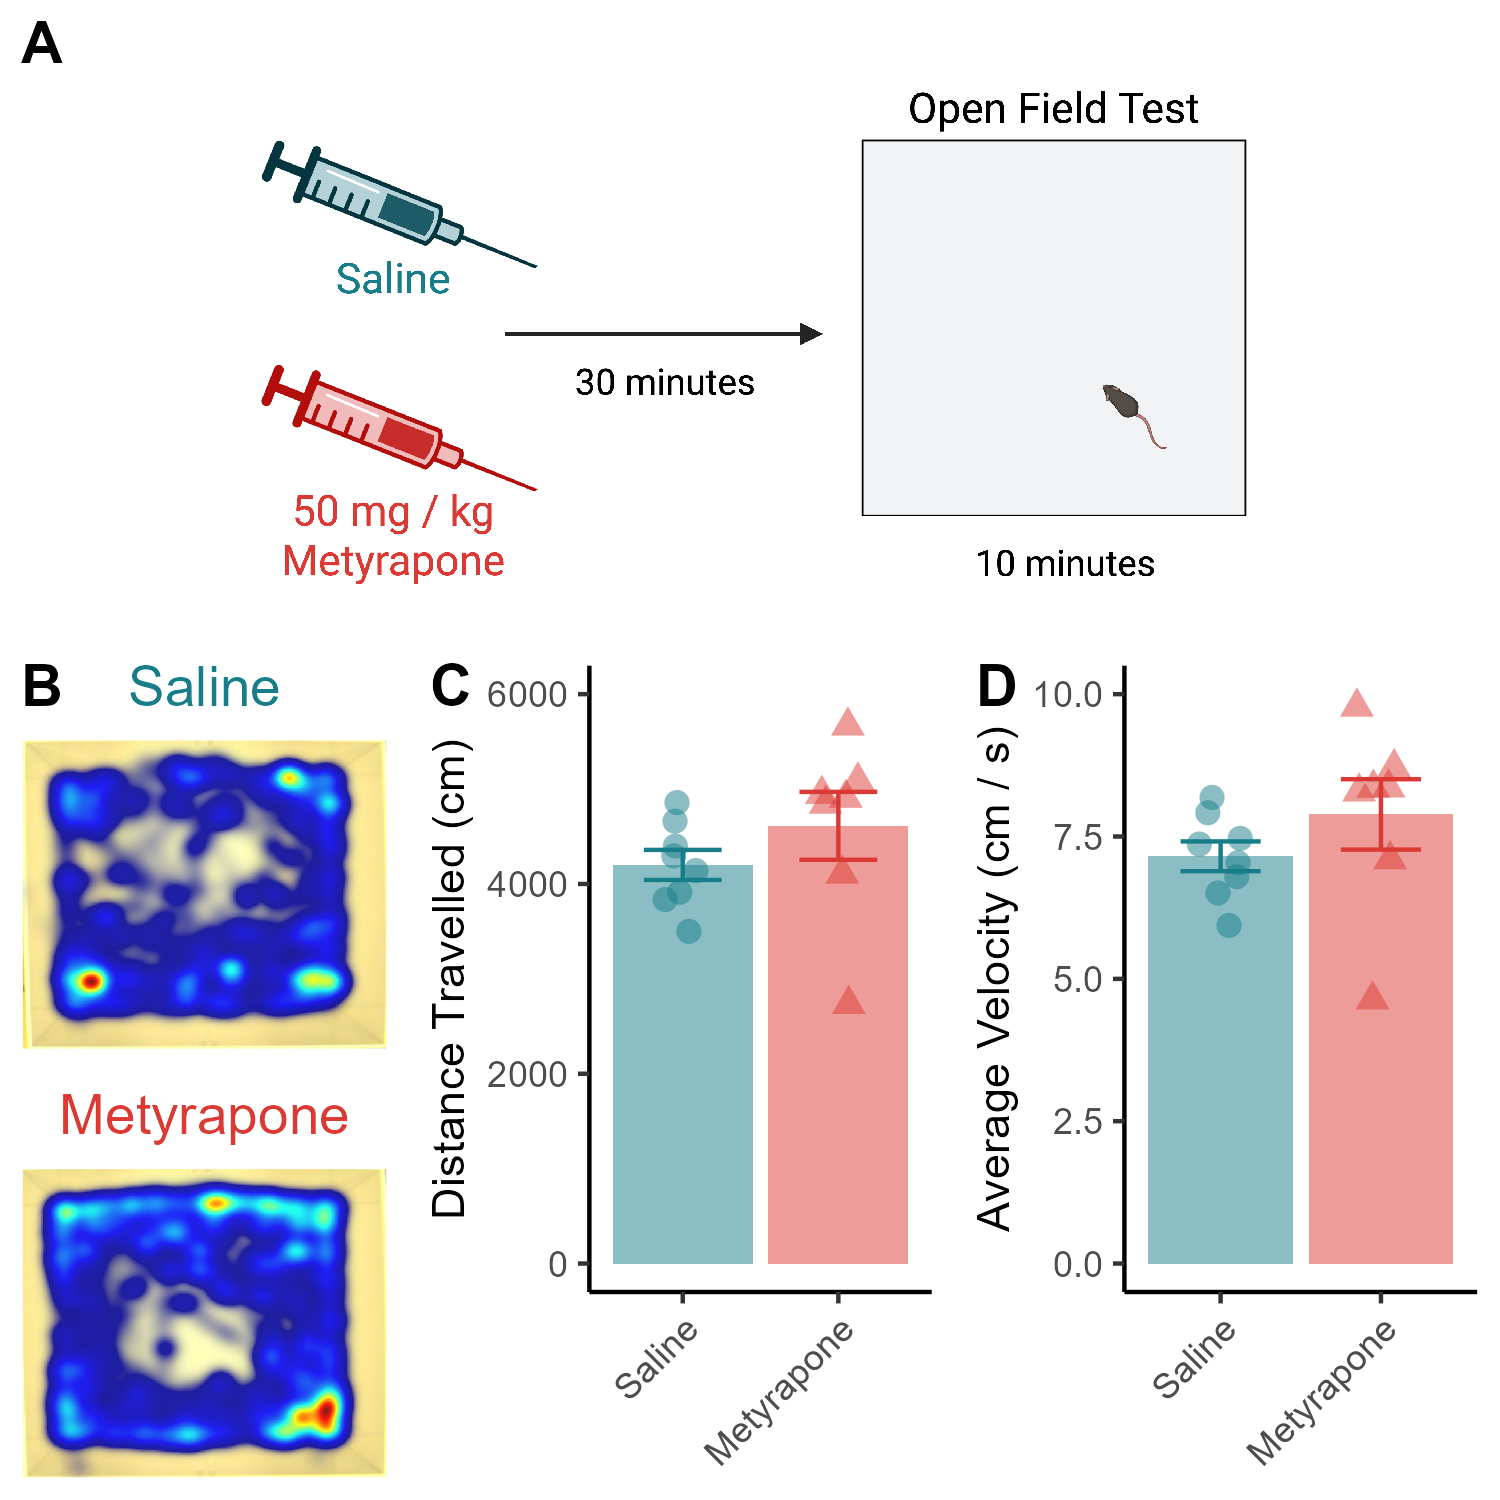
\includegraphics[width=20.83in]{Figs/S4_OFT}

\textbf{Supplemental Figure 4}. Metyrapone administration does not alter open field behavior. (A) Mice were injected with 50 mg / kg metyrapone 30 minutes before a 10-minute open field test. (B) Representative heatmaps of movement during the 10-minute session. (C) There was no effect of Metyrapone on total distance traveled during the task, and (D) average velocity was also not impacted by metyrapone. Data presented as mean value +/- SEM.

\begin{Shaded}
\begin{Highlighting}[]
\FunctionTok{t.test}\NormalTok{(Distance }\SpecialCharTok{\textasciitilde{}}\NormalTok{ Condition, }\AttributeTok{data =}\NormalTok{ data, }\AttributeTok{var.equal =}\NormalTok{ T)}
\end{Highlighting}
\end{Shaded}

\begin{verbatim}
## 
##  Two Sample t-test
## 
## data:  Distance by Condition
## t = 1.1024, df = 13, p-value = 0.2903
## alternative hypothesis: true difference in means between group Metyrapone and group Saline is not equal to 0
## 95 percent confidence interval:
##  -395.3512 1219.2112
## sample estimates:
## mean in group Metyrapone     mean in group Saline 
##                  4612.47                  4200.54
\end{verbatim}

\begin{Shaded}
\begin{Highlighting}[]
\FunctionTok{t.test}\NormalTok{(Velocity }\SpecialCharTok{\textasciitilde{}}\NormalTok{ Condition, }\AttributeTok{data =}\NormalTok{ data, }\AttributeTok{var.equal =}\NormalTok{ T)}
\end{Highlighting}
\end{Shaded}

\begin{verbatim}
## 
##  Two Sample t-test
## 
## data:  Velocity by Condition
## t = 1.1501, df = 13, p-value = 0.2708
## alternative hypothesis: true difference in means between group Metyrapone and group Saline is not equal to 0
## 95 percent confidence interval:
##  -0.646531  2.118472
## sample estimates:
## mean in group Metyrapone     mean in group Saline 
##                 7.888036                 7.152065
\end{verbatim}

Administration of 50 mg / kg metyrapone did not alter distance traveled in the open field (p = 0.29) or the average velocity of metyrapone-injected mice compared to saline-injected controls (p = 0.27; Figure S4).

\chapter*{Supplemental Figure 5}\label{supplemental-figure-5}
\addcontentsline{toc}{chapter}{Supplemental Figure 5}

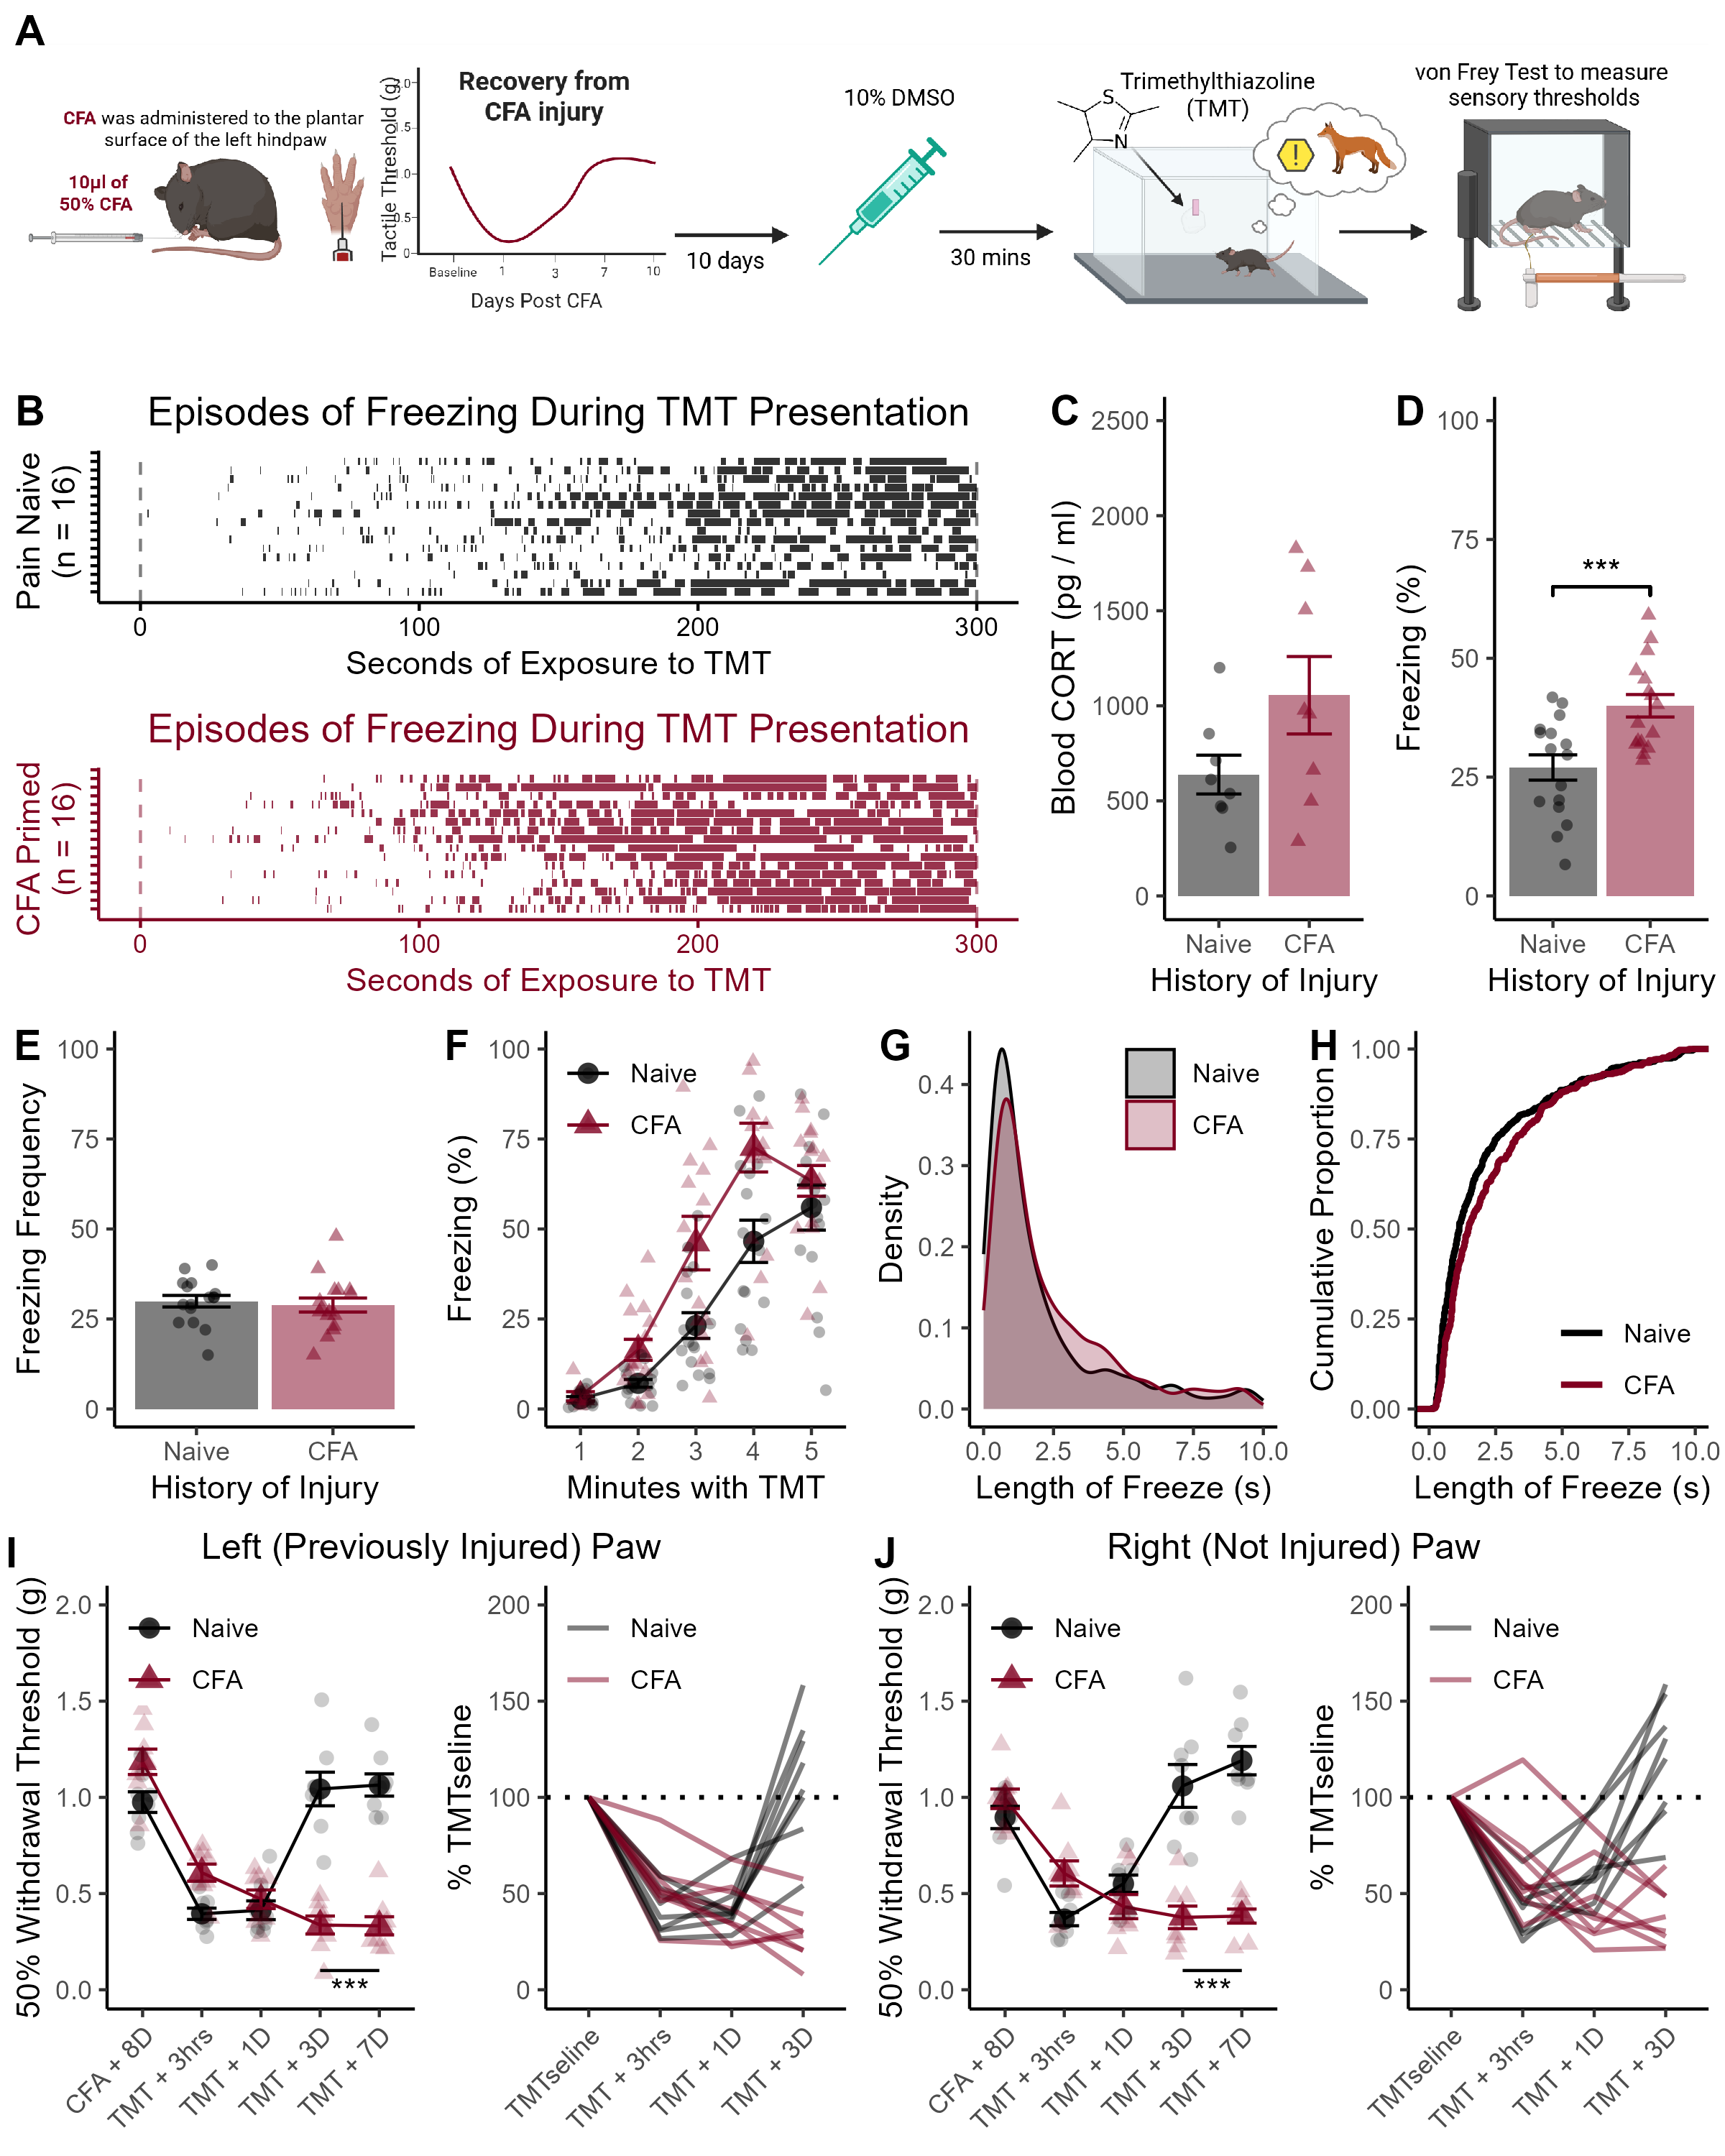
\includegraphics[width=33.33in]{Figs/S5_DMSO_Panel}

\textbf{Supplemental Figure 5}. Behavioral, hormonal and sensory responses to TMT after DMSO administration. (A) Timeline of experimental proceedings. Injury-naive controls and mice that had previously been injured with CFA and allowed to recover were administered 10\% DMSO 30 minutes before exposure to TMT. (B) Raster plots of individual bouts of freezing during TMT exposure. (C) Blood levels of CORT 30 minutes after TMT. (D) Average time spent freezing during TMT. (E) Time spent freezing broken down by minute. (F) Number of freezing episodes during TMT. (G) Density plot of individual bouts of freezing during TMT. (H) Cumulative proportion of individual bouts of freezing across the session. (I) Mechanical hypersensitivity among mice with a history of CFA at the site of previous injury. (J) Expression of mechanical hypersensitivity was also expressed in the contralateral (no previously injured) hind paw for mice with a history of CFA. Data presented as mean value +/- SEM.

\section*{CORT Levels}\label{cort-levels-1}
\addcontentsline{toc}{section}{CORT Levels}

\begin{Shaded}
\begin{Highlighting}[]
\FunctionTok{t.test}\NormalTok{(}\AttributeTok{data =}\NormalTok{ Cort\_data, CORT }\SpecialCharTok{\textasciitilde{}}\NormalTok{ CFA, }\AttributeTok{var.equal =}\NormalTok{ T)}
\end{Highlighting}
\end{Shaded}

\begin{verbatim}
## 
##  Two Sample t-test
## 
## data:  CORT by CFA
## t = -1.8313, df = 14, p-value = 0.08841
## alternative hypothesis: true difference in means between group Naive and group CFA is not equal to 0
## 95 percent confidence interval:
##  -905.95208   71.41745
## sample estimates:
## mean in group Naive   mean in group CFA 
##            638.2211           1055.4884
\end{verbatim}

The increased levels of blood-CORT among CFA-primed mice was not significant (p = 0.08).

\section*{Time Spent Freezing During TMT}\label{time-spent-freezing-during-tmt-2}
\addcontentsline{toc}{section}{Time Spent Freezing During TMT}

\begin{Shaded}
\begin{Highlighting}[]
\NormalTok{b }\OtherTok{\textless{}{-}}\NormalTok{ Exp\_1\_CFA.N  }\SpecialCharTok{\%\textgreater{}\%}
  \FunctionTok{filter}\NormalTok{(Behavior }\SpecialCharTok{==} \StringTok{"freeze"}\NormalTok{) }\SpecialCharTok{\%\textgreater{}\%}
  \FunctionTok{group\_by}\NormalTok{(ID,CFA) }\SpecialCharTok{\%\textgreater{}\%}
  \FunctionTok{summarise}\NormalTok{(}
    \AttributeTok{sum=}\FunctionTok{sum}\NormalTok{(Duration),}
    \AttributeTok{Number=}\FunctionTok{n}\NormalTok{(),}
\NormalTok{  ) }\SpecialCharTok{\%\textgreater{}\%}
  \FunctionTok{mutate}\NormalTok{(}\AttributeTok{Perc =}\NormalTok{ (sum }\SpecialCharTok{/} \DecValTok{300}\NormalTok{)}\SpecialCharTok{*}\DecValTok{100}\NormalTok{) }\SpecialCharTok{\%\textgreater{}\%}
  \FunctionTok{mutate}\NormalTok{(}\AttributeTok{Av\_DUR =}\NormalTok{ (sum }\SpecialCharTok{/}\NormalTok{ Number)) }
\end{Highlighting}
\end{Shaded}

\begin{verbatim}
## `summarise()` has grouped output by 'ID'. You can override using the `.groups`
## argument.
\end{verbatim}

\begin{Shaded}
\begin{Highlighting}[]
\FunctionTok{t.test}\NormalTok{(Perc}\SpecialCharTok{\textasciitilde{}}\NormalTok{CFA,}\AttributeTok{data=}\NormalTok{b,}\AttributeTok{var.equal=}\ConstantTok{TRUE}\NormalTok{)}
\end{Highlighting}
\end{Shaded}

\begin{verbatim}
## 
##  Two Sample t-test
## 
## data:  Perc by CFA
## t = -3.6504, df = 30, p-value = 0.0009881
## alternative hypothesis: true difference in means between group Naive and group CFA is not equal to 0
## 95 percent confidence interval:
##  -20.247317  -5.719725
## sample estimates:
## mean in group Naive   mean in group CFA 
##            27.02331            40.00683
\end{verbatim}

CFA-primed mice spent more time freezing that injury-naive controls (t\textsubscript{30} = 3.65, p \textless0.001, figure S5D \& E)

\section*{Frequency of Freezing During TMT}\label{frequency-of-freezing-during-tmt-1}
\addcontentsline{toc}{section}{Frequency of Freezing During TMT}

\begin{Shaded}
\begin{Highlighting}[]
\NormalTok{b }\OtherTok{\textless{}{-}}\NormalTok{ Exp\_1\_CFA.N  }\SpecialCharTok{\%\textgreater{}\%}
  \FunctionTok{filter}\NormalTok{(Behavior }\SpecialCharTok{==} \StringTok{"freeze"}\NormalTok{) }\SpecialCharTok{\%\textgreater{}\%}
  \FunctionTok{group\_by}\NormalTok{(ID,CFA) }\SpecialCharTok{\%\textgreater{}\%}
  \FunctionTok{summarise}\NormalTok{(}
    \AttributeTok{sum=}\FunctionTok{sum}\NormalTok{(Duration),}
    \AttributeTok{Number=}\FunctionTok{n}\NormalTok{(),}
\NormalTok{  ) }\SpecialCharTok{\%\textgreater{}\%}
  \FunctionTok{mutate}\NormalTok{(}\AttributeTok{Perc =}\NormalTok{ (sum }\SpecialCharTok{/} \DecValTok{300}\NormalTok{)}\SpecialCharTok{*}\DecValTok{100}\NormalTok{)}
\end{Highlighting}
\end{Shaded}

\begin{verbatim}
## `summarise()` has grouped output by 'ID'. You can override using the `.groups`
## argument.
\end{verbatim}

\begin{Shaded}
\begin{Highlighting}[]
\FunctionTok{t.test}\NormalTok{(Number}\SpecialCharTok{\textasciitilde{}}\NormalTok{CFA,}\AttributeTok{data=}\NormalTok{b,}\AttributeTok{var.equal=}\ConstantTok{TRUE}\NormalTok{)}
\end{Highlighting}
\end{Shaded}

\begin{verbatim}
## 
##  Two Sample t-test
## 
## data:  Number by CFA
## t = 0.42099, df = 30, p-value = 0.6768
## alternative hypothesis: true difference in means between group Naive and group CFA is not equal to 0
## 95 percent confidence interval:
##  -4.091773  6.216773
## sample estimates:
## mean in group Naive   mean in group CFA 
##             29.9375             28.8750
\end{verbatim}

There was no difference in freezing frequency (p = 0.67, Figure S5F).

\section*{Length of Freezing Bouts}\label{length-of-freezing-bouts}
\addcontentsline{toc}{section}{Length of Freezing Bouts}

\begin{Shaded}
\begin{Highlighting}[]
\NormalTok{a }\OtherTok{\textless{}{-}}\NormalTok{ data }\SpecialCharTok{\%\textgreater{}\%}
  \FunctionTok{filter}\NormalTok{(Behavior }\SpecialCharTok{==} \StringTok{"freeze"}\NormalTok{)}

\NormalTok{cfa\_durations }\OtherTok{\textless{}{-}}\NormalTok{ a}\SpecialCharTok{$}\NormalTok{Duration[a}\SpecialCharTok{$}\NormalTok{CFA }\SpecialCharTok{==} \StringTok{"CFA"}\NormalTok{]}
\NormalTok{naive\_durations }\OtherTok{\textless{}{-}}\NormalTok{ a}\SpecialCharTok{$}\NormalTok{Duration[a}\SpecialCharTok{$}\NormalTok{CFA }\SpecialCharTok{==} \StringTok{"Naive"}\NormalTok{]}

\FunctionTok{library}\NormalTok{(kSamples)}
\FunctionTok{ad.test}\NormalTok{(cfa\_durations, naive\_durations)}
\end{Highlighting}
\end{Shaded}

\begin{verbatim}
## 
## 
##  Anderson-Darling k-sample test.
## 
## Number of samples:  2
## Sample sizes:  462, 479
## Number of ties: 607
## 
## Mean of  Anderson-Darling  Criterion: 1
## Standard deviation of  Anderson-Darling  Criterion: 0.75984
## 
## T.AD = ( Anderson-Darling  Criterion - mean)/sigma
## 
## Null Hypothesis: All samples come from a common population.
## 
##                AD   T.AD  asympt. P-value
## version 1: 11.603 13.954       1.3197e-06
## version 2: 11.700 14.101       1.1609e-06
\end{verbatim}

The length of freezing episodes were longer for CFA-primed mice (D = 0.14, p \textless{} 0.001; Figure S5G, H). Relative to non-injured controls

\section*{Von Frey Sensitivity}\label{von-frey-sensitivity}
\addcontentsline{toc}{section}{Von Frey Sensitivity}

\begin{Shaded}
\begin{Highlighting}[]
\NormalTok{data }\SpecialCharTok{\%\textgreater{}\%}
  \FunctionTok{filter}\NormalTok{(Paw }\SpecialCharTok{==} \StringTok{"Left"}\NormalTok{) }\SpecialCharTok{\%\textgreater{}\%}
  \FunctionTok{anova\_test}\NormalTok{(}\AttributeTok{dv =}\NormalTok{ VF, }\AttributeTok{between =}\NormalTok{ CFA, }\AttributeTok{within =}\NormalTok{ Test, }\AttributeTok{wid =}\NormalTok{ ID)}
\end{Highlighting}
\end{Shaded}

\begin{verbatim}
## ANOVA Table (type II tests)
## 
## $ANOVA
##     Effect DFn DFd      F        p p<.05   ges
## 1      CFA   1  14 28.452 1.05e-04     * 0.303
## 2     Test   4  56 41.981 3.08e-16     * 0.702
## 3 CFA:Test   4  56 39.826 9.13e-16     * 0.691
## 
## $`Mauchly's Test for Sphericity`
##     Effect     W     p p<.05
## 1     Test 0.381 0.219      
## 2 CFA:Test 0.381 0.219      
## 
## $`Sphericity Corrections`
##     Effect   GGe     DF[GG]    p[GG] p[GG]<.05   HFe     DF[HF]   p[HF]
## 1     Test 0.705 2.82, 39.5 4.51e-12         * 0.902 3.61, 50.5 7.5e-15
## 2 CFA:Test 0.705 2.82, 39.5 9.73e-12         * 0.902 3.61, 50.5 2.0e-14
##   p[HF]<.05
## 1         *
## 2         *
\end{verbatim}

\begin{Shaded}
\begin{Highlighting}[]
\NormalTok{data }\SpecialCharTok{\%\textgreater{}\%}
  \FunctionTok{filter}\NormalTok{(Paw }\SpecialCharTok{==} \StringTok{"Right"}\NormalTok{) }\SpecialCharTok{\%\textgreater{}\%}
  \FunctionTok{anova\_test}\NormalTok{(}\AttributeTok{dv =}\NormalTok{ VF, }\AttributeTok{between =}\NormalTok{ CFA, }\AttributeTok{within =}\NormalTok{ Test, }\AttributeTok{wid =}\NormalTok{ ID)}
\end{Highlighting}
\end{Shaded}

\begin{verbatim}
## ANOVA Table (type II tests)
## 
## $ANOVA
##     Effect DFn DFd      F        p p<.05   ges
## 1      CFA   1  14 32.784 5.24e-05     * 0.368
## 2     Test   4  56 20.727 1.59e-10     * 0.527
## 3 CFA:Test   4  56 29.120 4.16e-13     * 0.610
## 
## $`Mauchly's Test for Sphericity`
##     Effect     W     p p<.05
## 1     Test 0.689 0.867      
## 2 CFA:Test 0.689 0.867      
## 
## $`Sphericity Corrections`
##     Effect   GGe     DF[GG]    p[GG] p[GG]<.05  HFe      DF[HF]    p[HF]
## 1     Test 0.825 3.3, 46.21 4.88e-09         * 1.11 4.44, 62.17 1.59e-10
## 2 CFA:Test 0.825 3.3, 46.21 3.53e-11         * 1.11 4.44, 62.17 4.16e-13
##   p[HF]<.05
## 1         *
## 2         *
\end{verbatim}

CFA-primed mice exhibited prolonged hypersensitivity in both the previously injured and the contralateral (not injured) hind paws after TMT exposure (Left Paw: F\textsubscript{4,56} = 39.82, p \textless{} 0.001; Right Paw: F\textsubscript{4,56} = 29.12, p \textless{} 0.001; Figure S5I \& J, respectively)

\chapter*{Supplemental Figure 6}\label{supplemental-figure-6}
\addcontentsline{toc}{chapter}{Supplemental Figure 6}

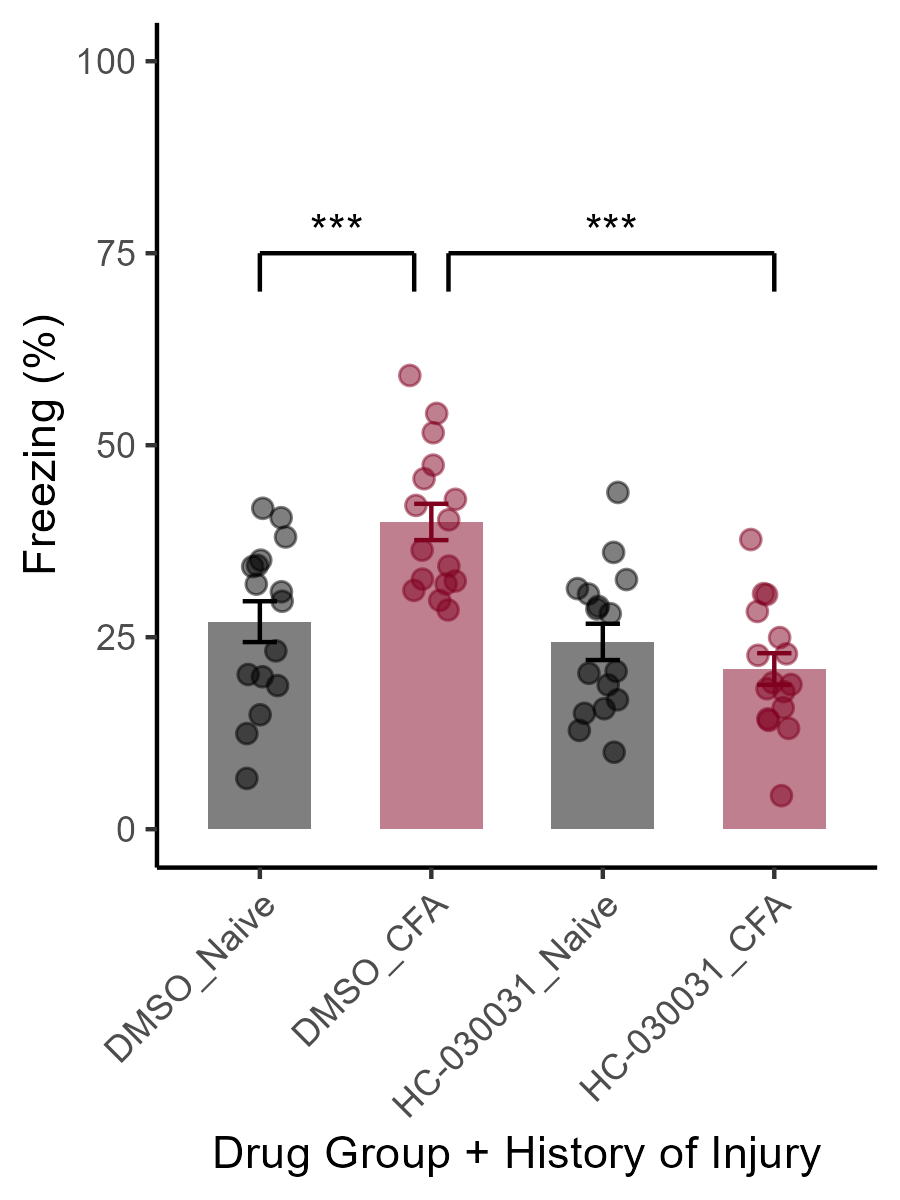
\includegraphics[width=12.5in]{Figs/S6_DMSO_compare}

\textbf{Supplemental Figure 6}. Time spent freezing during a five-minute exposure to TMT. A history of CFA injury increased time spent freezing, and this increase was prevented by administration of HC30031. Data presented as mean value +/- SEM.

\begin{Shaded}
\begin{Highlighting}[]
\NormalTok{res }\OtherTok{\textless{}{-}} \FunctionTok{aov}\NormalTok{(Perc }\SpecialCharTok{\textasciitilde{}}\NormalTok{ CFA }\SpecialCharTok{*}\NormalTok{ Drug, }\AttributeTok{data =}\NormalTok{ b)}
\FunctionTok{summary}\NormalTok{(res)}
\end{Highlighting}
\end{Shaded}

\begin{verbatim}
##             Df Sum Sq Mean Sq F value   Pr(>F)    
## CFA          1    357   357.1    3.97 0.050885 .  
## Drug         1   1898  1898.5   21.10 2.29e-05 ***
## CFA:Drug     1   1091  1091.4   12.13 0.000932 ***
## Residuals   60   5398    90.0                     
## ---
## Signif. codes:  0 '***' 0.001 '**' 0.01 '*' 0.05 '.' 0.1 ' ' 1
\end{verbatim}

\begin{Shaded}
\begin{Highlighting}[]
\NormalTok{b }\SpecialCharTok{\%\textgreater{}\%}
  \FunctionTok{group\_by}\NormalTok{(CFA) }\SpecialCharTok{\%\textgreater{}\%}
  \FunctionTok{pairwise\_t\_test}\NormalTok{(Perc }\SpecialCharTok{\textasciitilde{}}\NormalTok{ Drug)}
\end{Highlighting}
\end{Shaded}

\begin{verbatim}
## # A tibble: 2 x 10
##   CFA   .y.   group1 group2       n1    n2       p p.signif   p.adj p.adj.signif
## * <fct> <chr> <chr>  <chr>     <int> <int>   <dbl> <chr>      <dbl> <chr>       
## 1 Naive Perc  DMSO   HC-030031    16    16 4.65e-1 ns       4.65e-1 ns          
## 2 CFA   Perc  DMSO   HC-030031    16    16 1.04e-6 ****     1.04e-6 ****
\end{verbatim}

\begin{Shaded}
\begin{Highlighting}[]
\NormalTok{b }\SpecialCharTok{\%\textgreater{}\%}
  \FunctionTok{group\_by}\NormalTok{(Drug) }\SpecialCharTok{\%\textgreater{}\%}
  \FunctionTok{pairwise\_t\_test}\NormalTok{(Perc }\SpecialCharTok{\textasciitilde{}}\NormalTok{ CFA)}
\end{Highlighting}
\end{Shaded}

\begin{verbatim}
## # A tibble: 2 x 10
##   Drug     .y.   group1 group2    n1    n2       p p.signif   p.adj p.adj.signif
## * <fct>    <chr> <chr>  <chr>  <int> <int>   <dbl> <chr>      <dbl> <chr>       
## 1 DMSO     Perc  Naive  CFA       16    16 9.88e-4 ***      9.88e-4 ***         
## 2 HC-0300~ Perc  Naive  CFA       16    16 2.69e-1 ns       2.69e-1 ns
\end{verbatim}

\bibliography{book.bib,packages.bib}

\end{document}
